%   A flag and the \newif definition we will need to use it:
%               \Draft gives draft output
%               \Final gives final output
\newif\ifDraft\
\def\Draft{\Drafttrue}
\def\Final{\Draftfalse}
\Final\ % Uncomment this for final output
%\Draft % Uncomment this for draft output
\ifDraft\
\documentclass[12pt,draft,a4paper]{report}
\else
\documentclass[12pt,a4paper]{report}
\fi

%%%%%%%%%%%%%%%%%%%%%% Preamble %%%%%%%%%%%%%%%%%%%%%%%%%

\includeonly{standardPreamble,frontMasters,abstractMasters,thanksMasters,introductionMasters,j1655Masters,reductionMasters,elcMasters,conclusionMasters,irafMasters,diskMasters,lightcurveMasters}

\renewcommand{\baselinestretch}{1.4}
\setlength{\evensidemargin}{-1.0mm}
\setlength{\oddsidemargin}{15mm}
\setlength{\textwidth}{145mm}
\setlength{\topmargin}{-12mm}
\setlength{\headsep}{8mm}
\setlength{\textheight}{230mm}
\setlength{\footskip}{20mm}

% Define space between paragraphs
\newlength{\myparskip}
% Set space between paragraphs to 5mm
\setlength{\myparskip}{5mm}

% For time printing
\newcounter{hours}\newcounter{minutes}

\usepackage{latexsym}	% Symbol environment
\usepackage{ifthen}	% For operating system switches
\usepackage{calc}	% For time printing
\usepackage{varioref}	% For page-sensitive references
\usepackage{graphicx}	% For graphics
\usepackage{url}	% For urls
\usepackage{paralist}	% For different types of lists
\usepackage{astrobib}	% For aa style 
\usepackage{fixfoot}	% For multiple references to same footnote
\usepackage{xspace}	% To prevent problems with missing spaces

% Switch for operating system - 0 (Linux), 1 (Mac).
\newcounter{OS}
\setcounter{OS}{0}

% Hyphenation rules
\hyphenation{ FORTRAN Ve-ne-zue-la se-par-a-tion}

%% New Commands
%
\newcommand{\sun}{\ensuremath{_{\odot}}\xspace}
\newcommand{\degr}{\hbox{$^\circ$}\xspace}
\newcommand{\arcmin}{\hbox{$^\prime$}\xspace}
\newcommand{\arcsec}{\hbox{$^{\prime\prime}$}\xspace}
\newcommand{\fd}{\hbox{$.\!\!^{\rm d}$}}
\newcommand{\fh}{\hbox{$.\!\!^{\rm h}$}}
\newcommand{\fm}{\hbox{$.\!\!^{\rm m}$}}
\newcommand{\fs}{\hbox{$.\!\!^{\rm s}$}}
\newcommand{\fdg}{\hbox{$.\!\!^\circ$}}
\newcommand{\farcm}{\hbox{$.\mkern-4mu^\prime$}}
\newcommand{\farcs}{\hbox{$.\!\!^{\prime\prime}$}}
\newcommand{\fp}{\hbox{$.\!\!^{\scriptscriptstyle\rm p}$}}
%
% From LaTex Intro Book
%
\newcommand{\Chi}{\raisebox{0.4ex}{$\chi$}\xspace}
\newcommand{\lsim}{\mathrel{\hbox{\rlap{\lower.55ex\hbox{$\sim$}}
\kern-.3em \raise.4ex \hbox{$<$}}}}
\newcommand{\gsim}{\mathrel{\hbox{\rlap{\lower.55ex\hbox{$\sim$}}
\kern-.3em \raise.4ex \hbox{$>$}}}}
%
% From LaTeX Companion
\newcommand{\Printtime}{\setcounter{hours}{\time/60}%
	\setcounter{minutes}{\time-\value{hours}*60}%
	\ifthenelse{\value{hours}<10}{0}{}\thehours:%
	\ifthenelse{\value{minutes}<10}{0}{}\theminutes}

% From TeX FAQs
% Thick lines in tables
\setlength{\doublerulesep}{\arrayrulewidth}



\renewcommand{\reftextbefore}{on the previous page}%

\newcommand{\groj}{\mbox{GRO J1655--40}\xspace}
\newcommand{\nova}{\mbox{Nova Scorpii 1994}\xspace}
\newcommand{\iraf}{\texttt{IRAF}\xspace}

%%%%%%%%%%%%%%%%%%%%%% Body %%%%%%%%%%%%%%%%%%%%%%%%%

\begin{document}

\thispagestyle{empty}

%%%%%%%%%%%%%%%%%%%%%%%%%%%%% Title %%%%%%%%%%%%%%%%%%%%

\begin{center}


\textbf{Infrared Observations of \groj:\\ Constraints on the Black Hole Mass}

\vspace{15mm}

Francis Thomas O'Donovan, B.Sc.

\vspace{35mm}


Thesis for the Degree of M.Sc.\\
\vspace{5mm}
submitted to \\
\vspace{5mm}
the National University of Ireland, Cork.

\vspace{20mm}

Research conducted at \\
\vspace{5mm}
the Department of Physics, \\
\vspace{5mm}
National University of Ireland, Cork.

\vspace{30mm}

Submission date: October 2003

\vspace{15mm}


Head of Department: Prof.~S.~Fahy\\
\vspace{5mm}
Research Supervisor: Dr.~P.~J.~Callanan

\end{center}


\pagenumbering{roman}
\setcounter{page}{1}

\tableofcontents

%%%%%%%%%%%%%%%%%%%%%%%%%%%%% Abstract %%%%%%%%%%%%%%%%%%%%

\begin{center}
\Large{\textbf{Abstract}}
\end{center}

\vspace{\myparskip}

We present $K_s$-- and $J$--band photometry of \groj\ during two epochs
of observation, and determine the dereddened and absolute magnitudes
of this star system. We derive a range of spectral types (F0--G2 III--IV) for the secondary star
in \groj, using our $J_{0}-K_{0}$ colour estimate for this soft X--ray transient. We find the absolute
magnitude of \groj\ to be similar to that of another long period soft
X--ray transient. %

\vspace{\myparskip}

The first high signal--to--noise $K$--band spectrum of a black hole X--ray
transient system (\groj) is presented. This is used to show that the quiescent contribution of the accretion disk in \groj\
to the total flux of the system in the $K$--band is negligible. We are
therefore able to measure with certainty the binary inclination from the light curve of this stellar system, and place real bounds on the mass of the primary star in \groj. \groj\ is also shown to have
a similar spectrum to that of an F5--F7 III--IV star. %

\vspace{\myparskip}

The ellipsoidal modulation observed in the $K_s$--band is modelled
using \textit{ELC}, to obtain an inclination of $64\degr$--$70\degr$ and a mass ratio of $2.5$--$6$ for the system. These values concur with past results. The derived primary mass, $M_X =
6.8\pm0.7$\,M\sun, suggests that the compact object in \groj\ is a black
hole. %

\vspace{\myparskip}

An attempt is made to model the system in outburst, taking the
ellipsoidal variability of the secondary star and the eclipse of a bright
accretion disk into account. The resultant fit is poor, a consequence
of the asymmetries of the disk and flickering in the $K_s$--band. The
outburst light curve of \groj\ is shown to display an eclipse of the
accretion disk, consistent with the high inclination of the system. %


%%%%%%%%%%%%%%%%%%%%%%%%%%%%% Acknowledgements %%%%%%%%%%%%%%%%%%%%

\begin{center}
\Large{\textbf{Acknowledgements}}
\end{center}

\vspace{\myparskip}

I would like to express my heartfelt gratitude for the support and
advice of Dr.~Paul~Callanan. Throughout my undergraduate degree,
Dr.~Callanan encouraged my interest in astrophysics and provided me
with the opportunity to gain experience in this field. His supervision
of my M.Sc.\ has helped cement my interest and has given me valuable
skills and knowledge. I am also indebted to him for his help in both
selecting and securing a university place for my Ph.D.\ studies. %

\vspace{\myparskip}

My thanks must also be given to the U.C.C.\ Physics Department. The
academic staff have stimulated my mind for several years, while the
technical and clerical staff have helped me with more practical
matters. I must not forget my fellow students, especially Lisa Goggin,
all of whom have helped me struggle through five years of Physics. %

\vspace{\myparskip}

Thanks also to the present and former occupants of the Astrophysics
Laboratory. Manuel Perez-Torres generously spent a lot of time
explaining X--ray Binaries to me, in spite of the demands of his own
Ph.D. John~McCarthy and Peter~Curran have both helped
me in my research work and in the preparation of this document. %

\vspace{\myparskip}

Finally, my sincere gratitude to my parents, Tom and Vera, and my
sister, Bridget, who have supported and encouraged me throughout my
entire education, and also to my dearest Gillian, who was very
patient and understanding. %


\pagenumbering{arabic}

%%%%%%%%%%%%%%%%%%%%%% Chapters %%%%%%%%%%%%%%%%%%%%%%%%%


%%%%%%%%%%%%%%%%%%%%%%%%%%%%% Introduction %%%%%%%%%%%%%%%%%%%%

\chapter{Introduction}
\label{cha:Introduction}

This thesis is concerned with the study of an X--ray binary star
system,\\%
% WHITE SPACE %
\groj, which is thought to harbour a black hole. Before
discussing this particular system in detail, a general introduction is
given to black holes and X--ray binaries. %

%%%%%%%%%%%%%%%%%%%%%%%%%%%%% Black Holes %%%%%%%%%%%%%%%%%%%%

\section{Black Holes}
\label{cha:Introduction:sec:BlackHoles}

Possibly the most spectacular event in astrophysics is the death of a
``massive'' star, which is a star of mass greater than eight solar
masses. After millions of years of phenomenal energy output, the star
finally runs out of fuel. Most massive stars are then thought to form
dense cores, called \textbf{compact objects}, and some eventually
destroy themselves almost entirely. Such stars become a type of
compact objects called \textbf{black holes}. This section introduces
this exotic type of star and we will later explain the search for
evidence of the existence of black holes. %

\vspace{\myparskip}

Once a massive particle feels the gravitational attraction of a mass $M$, it
requires a certain velocity, called the \textbf{escape velocity
($v_{esc}$)}, to remove itself from that gravitational attraction. This
velocity is given by the formula:
\begin{equation}
\label{cha:Introduction:sec:BlackHoles:eqn:V_Esc}
v_{esc} = \sqrt{\frac{2 G M}{r}},
\end{equation}
where $r$ is the distance between the masses, and $G$ is the
Gravitational constant. At the end of the 18th Century, Michell and Laplace suggested the
possibility of massive stars with $v_{esc} > c$. (Here, $c$ is the
speed of light in a vacuum.) These objects would always appear as
black stars. With the development of Einstein's General Theory of
Relativity, the modern picture of these ``black holes'' evolved: it is
now thought that a black hole remnant is formed when a star of
mass greater than ten solar masses ends its life cycle with a direct gravitational collapse. %
The matter remaining in the core of the star is totally devoid of
nuclear fuel and hence is compressed by gravity until it converges to a singularity - a black hole. %

%%%%%%%%%%%%%%%%%%%%%%%%%%%%% The Event Horizon %%%%%%%%%%%%%%%%%%%%

\subsubsection{The Schwarzschild Radius: the Size of the Black Hole}
\label{cha:Introduction:sec:BlackHoles:subsubsec:EventHorizon}

It is thought that each black hole is surrounded by an \textbf{event
horizon}. This imaginary surface signifies the point of no return for any particle of mass
or radiation: once the particle has passed beyond the event horizon,
it is forever bound to the black hole. Not even light can escape, once it crosses this surface. Hence the compact object appears ``black''. %

\vspace{\myparskip}

All the points on the event horizon are a certain distance from the black hole, called the
\textbf{Schwarzschild radius ($R_{Sch}$)}. %
At this radius, which is given by:
\begin{equation}
\label{cha:Introduction:sec:BlackHoles:eqn:R_Sch}
R_{Sch} = \frac{2 G M}{c^2},
\end{equation}
the escape velocity equals the speed of light. This radius is often used to characterise the size of the black hole -- these objects have no surface radius, being singularities. %

%%%%%%%%%%%%%%%%%%%%%%%%%%%%% How Can We Observe a Black Star in a Black Sky? %%%%%%%%%%%%%%%%%%%%

\subsubsection{How Can We Observe a Black Star in a Black Sky?}
\label{cha:Introduction:sec:BlackHoles:subsubsec:HowCanWeObserveABlackStarInABlackSky}

It is difficult to observe isolated black holes directly, as they emit
very little radiation. However, the gravitational field caused by the mass of
the black hole is more easily detected, especially if the black hole
is gravitionally bound to a nearby star. When two stars are bound
together like this by their mutual gravitational attraction, the pair is known
as a \textbf{binary system}. We will later explore the specifics of
binaries containing black holes, but we first briefly summarize various topics
related to binary systems in general. %

%%%%%%%%%%%%%%%%%%%%%%%%%%%%% Binary Star Systems %%%%%%%%%%%%%%%%%%%%

\section{Binary Star Systems}
\label{cha:Introduction:sec:BinaryStarSystems}

The majority of ``stars'' seen in the night sky are in fact multiple--star systems, each of which contain two or more mutually-bound stars. Here we examine the characteristics of binary star systems.

%%%%%%%%%%%%%%%%%%%%%%%%%%%%% Properties of a Binary System %%%%%%%%%%%%%%%%%%%%

\subsection{Properties of a Binary System}
\label{cha:Introduction:sec:BinaryStarSystems:subsec:Properties}

The relative positions of the two component
stars in a binary system to the observer is known as the
\textbf{orbital phase}. Because the two stars in a binary system are orbiting about a common
centre of gravity, the appearance of the system to an observer changes as the stars rotate, and the orbital phase of the system changes. (Figure~%
\vref{cha:Introduction:sec:X--rayBinaries:fig:PringlePhaseEdited}%
\ shows various different phases for a type of binary system known as a
\textbf{Cataclysmic Variable}%
). At \textbf{phase 0.0}, the observer sees the \textbf{secondary}
(less massive) star in front of the \textbf{primary} star, and at
\textbf{phase 0.5}, the secondary is behind. The primary star and secondary star are observed side by
side at \textbf{phases 0.25} and \textbf{0.75}: these phases are known
as the \textbf{quadratures}. (Phases 0.0 and 0.5 are similarly known
as the \textbf{conjunctions}.) Note the time taken for the binary
system to rotate through one complete cycle of phases is known as the \textbf{orbital period ($P$)}. %

\vspace{\myparskip}

The appearance of a binary system also depends on other properties of
the system, such as:
\begin{itemize}
\item
the \textbf{mass of the primary}, $M_1$, and the \textbf{mass of the secondary}, $M_2$ -- the quantity $q = M_{1}/M_{2}$ is known as the \textbf{mass ratio}, %
\item
the \textbf{angle of orbital inclination}, $i$, which is the angle
between the observer and the normal to the orbital plane , and %
\item
the \textbf{binary separation}, which is the distance between the two stars. %
\end{itemize}

%%%%%%%%%%%%%%%%%%%%%%%%%%%%% Ellipsoidal Variability %%%%%%%%%%%%%%%%%%%%

\subsection{Ellipsoidal Variability of a Distorted Star}
\label{cha:Introduction:sec:X--rayBinaries:subsec:EllipsoidalVariability}

When the binary separation of a system is roughly comparable to the
diameter of the star with the largest volume, the pair is called a
\textbf{close binary system}. %
The rotational and tidal forces acting on a star within a close binary
system can cause a stretching of the star into a tear-drop shaped
figure. In this thesis, most of the secondary stars in the systems we discuss are deformed in this way. %

\vspace{\myparskip}

This deformation of the secondary star can modulate the brightness of the binary system. %
The apparent flux of the secondary varies as a function of orbital phase, because this flux is
proportional to the projected surface area %
visible to the observer. As the binary system rotates, we see the projected surface area of the secondary star change (see, for example, Figure~%
\vref{cha:Introduction:sec:X--rayBinaries:fig:PringlePhaseEdited}%
). The amplitude of this variability depends primarily on the angle of inclination ($i$) and the mass ratio ($q$). It is largest for $i=90\degr$. %

\vspace{\myparskip}

For a given $i$, the projected surface area of the secondary star is
at its maximum value at the quadratures. The flux from the secondary is therefore at
its maximum value at phases 0.25 and 0.75. In a similar manner, the
flux is at its minimum values at the conjunctions, when the secondary is observed end-on and the
projected surface area is approximately circular. %

\vspace{\myparskip}

Under normal circumstances (e.g., the star is in hydrostatic
equilibrium), the local radiation flux on the surface of a star is
proportional to the local surface gravity. %
This gives rise to \textbf{gravitational darkening}. %
At \textbf{inferior conjunction} of the secondary (phase 0.0), the tidally-undisturbed side of the
secondary star faces the observer. All the points on the surface of
the star are equidistant from the centre of the star, and hence have the
same surface gravity and flux. %
However, at \textbf{superior conjunction} (phase 0.5), the star presents its distorted side, where the surface gravity is at its lowest, and hence the surface brightness
is also at its lowest value. This results in a deeper minimum in the light curve of the secondary star at phase 0.5 than at phase 0.0.

%%%%%%%%%%%%%%%%%%%%%%%%%%%%% OB97Figure6Edited2 %%%%%%%%%%%%%%%%%%%%
\begin{figure}[htb]
\begin{center}
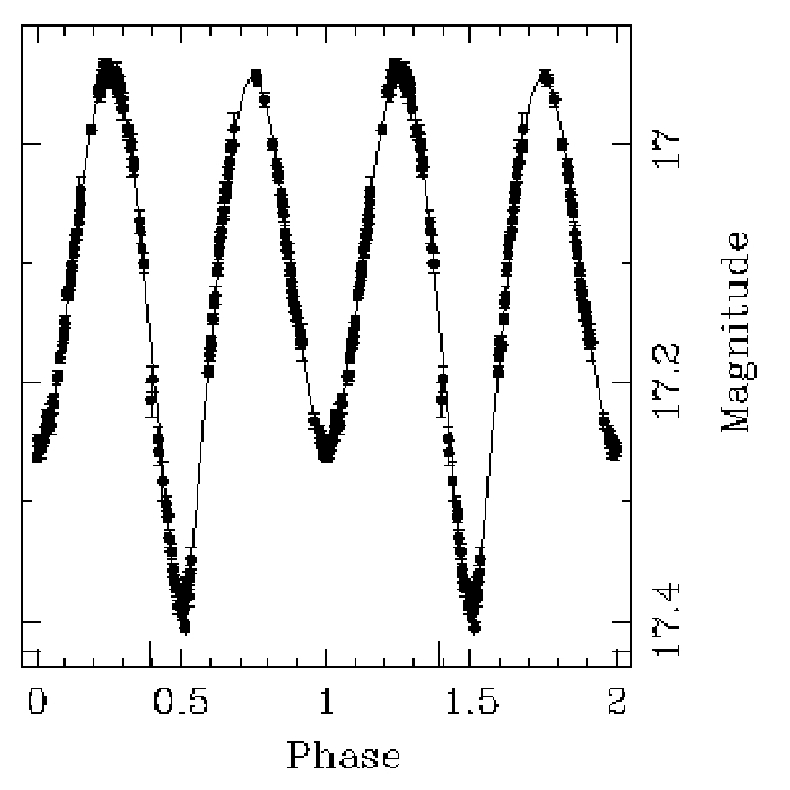
\includegraphics[width=9.2cm]{OB97Figure6Edited2}
\caption{%
Model fit to the optical light curve of the X--ray binary \groj,
showing the characteristic ellipsoidal variability of a distorted
secondary star. (Adapted from Orosz \& Bailyn 1997%
.)%
}
\label{cha:Introduction:sec:X--rayBinaries:subsec:EllipsoidalVariability:fig:OB97Figure6Edited2}
\end{center}
\end{figure}
\nocite{OroszBailyn:1997} %
%%%%%%%%%%%%%%%%%%%%%%%%%%%%%%%%%%%%%%%%%%%%%%%%%%%%%%%%%%%%%%%%%%

\vspace{\myparskip}

In a binary system whose flux is dominated by that of the secondary
star, the light curve of the system will show the same ellipsoidal
variation as the secondary. An example of this \textbf{ellipsoidal
variability}, also known as \textbf{double hump modulation}, is given in Figure~%
\vref{cha:Introduction:sec:X--rayBinaries:subsec:EllipsoidalVariability:fig:OB97Figure6Edited2}%
. %

%%%%%%%%%%%%%%%%%%%%%%%%%%%%% Eclipses %%%%%%%%%%%%%%%%%%%%

\subsection{Eclipses in a Binary System}
\label{cha:Introduction:sec:X--rayBinaries:subsec:Eclipses}

%%%%%%%%%%%%%%%%%%%%%%%%%%%%% WDEclipsing %%%%%%%%%%%%%%%%%%%%
\begin{figure}[!htb]
\begin{center}
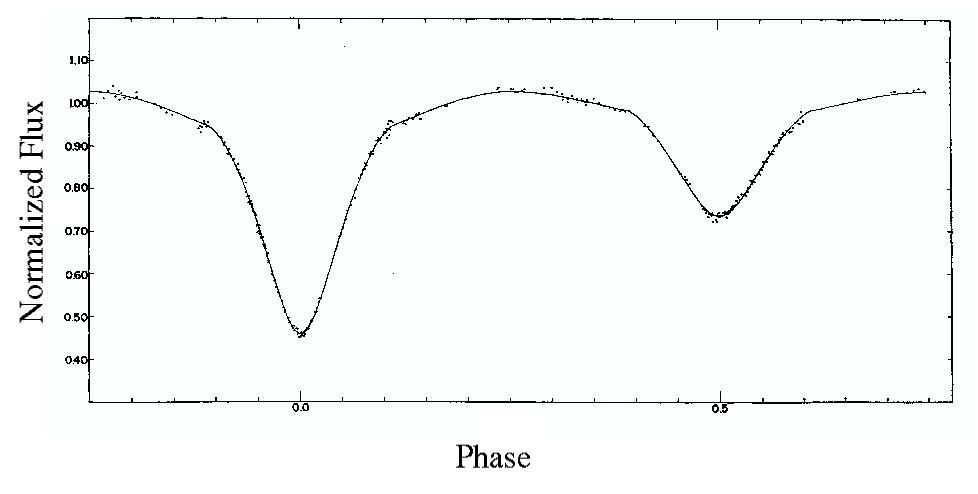
\includegraphics[width=15.0cm]{WDEclipsing}
\caption{%
Observations of the eclipsing binary WR Cyg, overplotted with a theoretical light curve. %
(Adapted from Wilson \& Devinney~1971.)%
}
\label{cha:Introduction:sec:X--rayBinaries:subsec:Eclipses:fig:WDEclipsing}
\end{center}
\end{figure}
\nocite{WilsonDevinney:1971} %
%%%%%%%%%%%%%%%%%%%%%%%%%%%%%%%%%%%%%%%%%%%%%%%%%%%%%%%%%%%%%%%%%%



Another property of the light curve of a binary system is the presence
or absence of \textbf{eclipses}. When the orbital inclination of a binary system is high enough, the component stars in the system will travel in front of each other as they orbit the centre
of mass of the system. Since the closer star blocks the light of the
further, the total flux from the system diminishes. These \textbf{eclipses} may be the most prominent features of the light curve of the
binary. Of course, if the inclination is too low, no eclipses will
occur. Therefore, the presence or absence of eclipses puts a limit on
the value of the orbital inclination. Figure~%
\vref{cha:Introduction:sec:X--rayBinaries:subsec:Eclipses:fig:WDEclipsing}%
\ shows a model of an eclipsing system with the resultant light
curve. %

%%%%%%%%%%%%%%%%%%%%%%%%%%%%% Accretion %%%%%%%%%%%%%%%%%%%%

\subsection{Accretion onto the Primary}
\label{cha:Introduction:sec:BinaryStarSystems:subsec:Accretion}

An important effect of the deformation of the secondary star in a close binary is the possible transfer of mass from one star to the other. This process is known as \textbf{accretion} or \textbf{mass transfer}. Whether it occurs depends on the sizes and separation of the component stars, as we now explain.%

%%%%%%%%%%%%%%%%%%%%%%%%%%%%% The Roche Lobes %%%%%%%%%%%%%%%%%%%%

\subsubsection{Accretion and the Roche Lobes}
\label{cha:Introduction:sec:BinaryStarSystems:subsec:Accretion:subsubsec:RocheLobes}

During the 19th century, the French mathematician Edouard Roche
studied the interactions of planetary satellites. %
His work has been applied to binary systems to develop a theoretical
model for accretion.

%%%%%%%%%%%%%%%%%%%%%%%%%%%%% PringleRoche %%%%%%%%%%%%%%%%%%%%
\begin{figure}[!htb]
\begin{center}
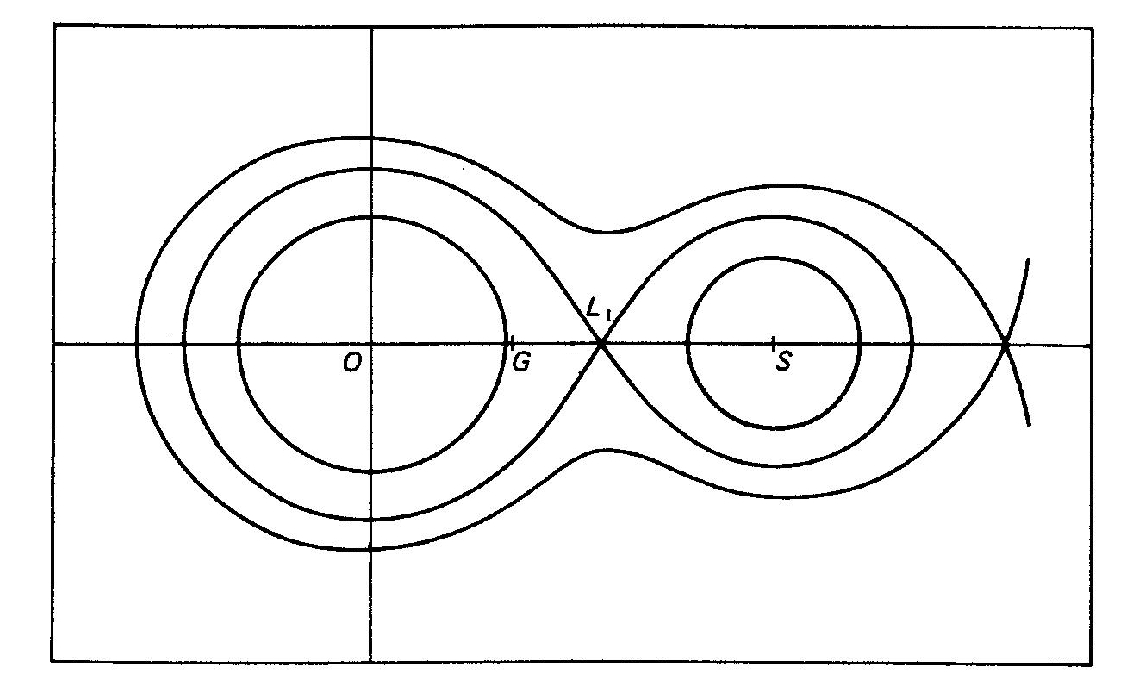
\includegraphics[width=10.0cm]{PringleRoche}
\caption{%
Example of the Roche equipotentials for a binary system.  The centre,
$O$, of the primary star is marked, as is
the centre, $S$, of the secondary star.  Also marked are
the Lagrangian point, $L_1$, and the centre of mass, $G$, of the
system. The mass ratio is given as $q = 2$. %
(Adapted from Pringle~1985.)%
}
\label{cha:Introduction:sec:BinaryStarSystems:subsec:Accretion:subsubsec:RocheLobes:fig:PringleRoche}
\end{center}
\end{figure}
\nocite{Pringle:1985} %
%%%%%%%%%%%%%%%%%%%%%%%%%%%%%%%%%%%%%%%%%%%%%%%%%%%%%%%%%%%%%%%%%%

\vspace{\myparskip}

By studying the gravitational interaction between two objects, Roche
developed a series of curves representing equipotential surfaces
surrounding the pair (see Figure~%
\vref{cha:Introduction:sec:BinaryStarSystems:subsec:Accretion:subsubsec:RocheLobes:fig:PringleRoche}). The shape and size of these curves are determined by the mass ratio of
the two objects and their separation.  The most important curves are
the two so-called \textbf{Roche lobes}, the ``figure of 8'' shaped surface. %

\vspace{\myparskip}

As the \textbf{companion} (secondary) star evolves, %
its size increases and it may expand to fill its Roche lobe. Some of
the matter of that star may lie on or even outside this lobe, and some of this matter will
be attracted towards the primary. The gas will flow towards the
primary through the \textbf{inner Lagrangian point ($L_1$)}, %
which is the intersection of the Roche lobes. This process is known as
\textbf{Roche lobe overflow accretion}. %
Such a binary system is known as a \textbf{semi-detached binary}, if the radius of the primary star is less than its Roche lobe
radius. If the companion star of a binary system does not fill its
Roche lobe, then the stellar matter is bound and no mass transfer to
the primary occurs by Roche lobe accretion. In some such systems, mass
transfer can still occur via a
\textbf{stellar wind}, a stream of gas particles flowing out from the star, similar to the
solar wind. In this thesis, however, we are mainly concerned with
Roche lobe overflow accretion. %

\vspace{\myparskip}

The characteristics of binary systems that we have outlined are common to all binaries -- we now detail the specifics of the type of binary systems known as X--ray binaries. %

%%%%%%%%%%%%%%%%%%%%%%%%%%%%% X--ray Binaries %%%%%%%%%%%%%%%%%%%%

\section{X--ray Binaries}
\label{cha:Introduction:sec:X--rayBinaries}

%%%%%%%%%%%%%%%%%%%%%%%%%%%%% PringlePhaseEdited %%%%%%%%%%%%%%%%%%%%
\begin{figure}[htb]
\begin{center}
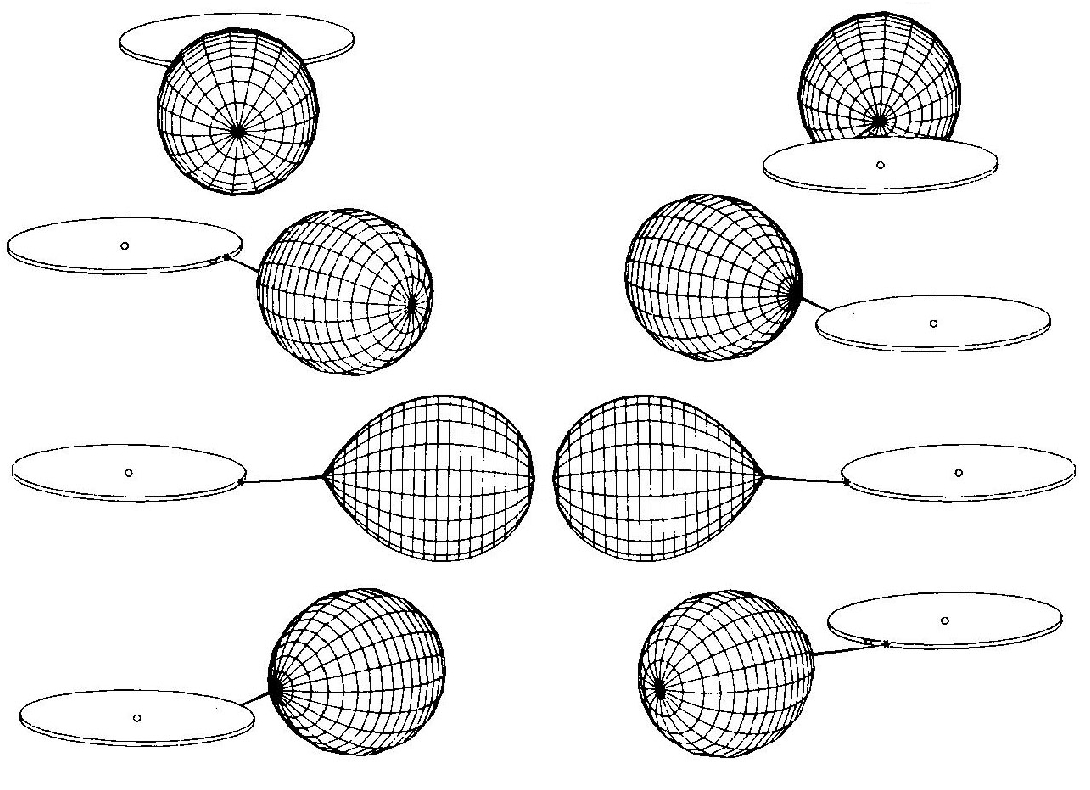
\includegraphics[width=10.0cm]{PringlePhaseEdited}
\caption{%
The observed relative positions of the component stars of a cataclysmic variable
as a function of orbital phase, beginning with phase 0.0. The
phase difference between images, going from top to bottom, is
0.125. (Adapted from %
Pringle \& Wade 1985.)%
}
\label{cha:Introduction:sec:X--rayBinaries:fig:PringlePhaseEdited}
\end{center}
\end{figure}
\nocite{PringleWade:1985} %
%%%%%%%%%%%%%%%%%%%%%%%%%%%%%%%%%%%%%%%%%%%%%%%%%%%%%%%%%%%%%%%%%%

Many semi-detached binary systems have a compact primary star and a
non-degenerate secondary. (For the remainder of this discussion, such a
binary system will be assumed unless otherwise stated.) This compact
object may be a white dwarf, neutron star or black hole.

\vspace{\myparskip}

When the primary star of such a system is an accreting white dwarf, the system is a \textbf{cataclysmic variable} (see Figure~\vref{cha:Introduction:sec:X--rayBinaries:fig:PringlePhaseEdited} for an example): these variables are divided into such categories as the brighter \textbf{classical
  novae}, the fainter \textbf{dwarf novae}%
\label{cha:Introduction:sec:X--rayBinaries:subsec:CompactObjects:topic:DwarfNovae}%
 and the \textbf{novalike objects}. %
The radiation emitted by these systems is chiefly in the optical and ultraviolet regions
of the electromagnetic spectrum. %

When the primary in a close binary system is a neutron star or
black hole, the binary is called an \textbf{X--ray binary}.
X--ray binaries take their name from the fact that the majority of
the energy radiated from the bright systems during phases of high accretion is in the form of X--rays (with
energies 0.1--100\,keV). (We denote the mass of this X--ray emitting object by $M_{X}$.) In an X--ray binary, the radius of the compact primary will always be
less than its Roche lobe radius, hence these systems are
always semi-detached.


\vspace{\myparskip}

In 1962, Giacconi et~al.\ discovered the first known X--ray emitting cosmic
object in the constellation of Scorpius (Giacconi et~al.\ %
\citeyearNP{Giacconi_et_al.:1962}). %
The source, christened Sco X--1, was later shown to be a binary
system, and is usually the brightest X--ray binary in the sky. The
first confirmed X--ray binary, however, was \mbox{Cyg X--1} %
\cite{WebsterMurdin:1972,Bolton:1972}. %
Since this observation, approximately 300 X--ray binaries have been
identified %
(\citeNP{LiuVanParadijsVanDenHeuvel:2000},
\citeNP{LiuVanParadijsVanDenHeuvel:2001}).%

\vspace{\myparskip}

Once the first X--ray binaries had been identified optically, their
distances and hence their intrinsic X--ray luminosities were determined. Some of the luminosities calculated were of the order of $10^{31}\,\mathrm{W}$, which is approximately
$10^5\,\mathrm{L}\sun$ (where $\mathrm{L}\sun$ is the
luminosity of the Sun%
\footnote{%
\label{cha:Introduction:sec:X--rayBinaries:foot:Lsun}
$1\,\mathrm{L}\sun = 3.826 \times 10^{26}\,\mathrm{W}$ }%
). %
\label{cha:Introduction:sec:X--rayBinaries:subsec:CompactObjects:topic:HighLum}
\citeN{Shklovsky:1967:ApJL} %
suggested that this unusually high luminosity of X--ray binaries such as
Sco X--1 could be accounted for if they were mass-exchanging binaries
with a neutron star component. %
This was the first realisation that accretion was an important power
source. Much of the energy radiated by these systems comes from a disk of gas around the primary star -- the \textbf{accretion disk}.

%%%%%%%%%%%%%%%%%%%%%%%%%%%%% Accretion Disk %%%%%%%%%%%%%%%%%%%%

\subsection{The Accretion Disk}
\label{cha:Introduction:sec:BinaryStarSystems:subsec:AccretionDisk}

In a binary where accretion is taking place, if there is a continual stream of particles flowing from the
the secondary star to the primary, the gas forms a disk, known as the
\textbf{accretion disk}. %
The rotation of the secondary star imparts angular momentum to the matter flowing into this disk.
Viscous processes redistribute the angular momentum amongst the
gas particles, which causes the in--falling of some of the particles onto the primary. The in--falling
gas is heated until it forms a highly ionized plasma, with highest
temperatures closest to the primary. %

\vspace{\myparskip}

An accretion disk is very efficient at converting the gravitational potential energy of the transferred matter into radiation. For example, about 20\% (for a neutron star primary) or 30\% (for a
black hole primary) of the rest energy of the accreted gas may be
emitted as radiation. The accretion results in a luminosity of the primary given by:
\begin{equation}
\label{cha:Introduction:sec:X--rayBinaries:subsec:AccretionDisk:eqn:LumAcc}
L = \frac{G M_X \dot{m}}{R_X},
\end{equation}
where $R_X$ is the radius of the primary star, and $\dot{m}$ is the
rate of mass transfer from the secondary star onto the primary star. %
(Note that this formula does not strictly apply to black holes, as it assume a
primary star with a hard surface.) %
There exists an upper limit for $L$, called the \textbf{Eddington
Limit ($L_{E}$)}%
\label{cha:Introduction:sec:BinaryStarSystems:subsec:AccretionDisk:topic:L_E}%
, above which the outer parts of the star cannot remain in hydrostatic
equilibrium. Above $L_{E}$, the process of accretion is halted due to
the radiative pressure from the star, and in fact mass loss from the primary may occur. %

\vspace{\myparskip}

Using Equation~%
\vref{cha:Introduction:sec:X--rayBinaries:subsec:AccretionDisk:eqn:LumAcc}, %
and assuming a solar mass primary, we see
that the high luminosities mentioned on page~%
\pageref{cha:Introduction:sec:X--rayBinaries:subsec:CompactObjects:topic:HighLum}%
\ can be generated by an accretion rate of
only $10^{-8}\,\mathrm{M}\sun\,\mathrm{yr^{-1}}$ (e.g., %
\citeNP{Fabian:1985}%
), %
reflecting the aforementioned efficiency of accretion as a power
source. (Here $\mathrm{M}\sun$\ is the mass of the Sun%
\footnote{%
\label{cha:Introduction:sec:X--rayBinaries:foot:Msun}
$1\,\mathrm{M}\sun = 1.99 \times 10^{30}\,\mathrm{kg}$}%
.)

%%%%%%%%%%%%%%%%%%%%%%%%%%%%% Reprocessing of Radiation %%%%%%%%%%%%%%%%%%%%

\subsubsection{Reprocessing of Radiation}
\label{cha:Introduction:sec:X--rayBinaries:subsec:AccretionDisk:subsubsec:ReprocessingOfRadiation}

An important effect of accretion in the case of X--ray binaries is a
process called \textbf{X--ray reprocessing} or \textbf{X--ray heating}. The X--ray radiation emitted by the
accreting material interacts with the matter in the accretion disk, in
the secondary star or surrounding the binary system. This interaction
converts some of the emission into optical and infrared (IR) radiation. This
X--ray heating can affect the appearance of the disk and the secondary
star, as we will later see. %

%%%%%%%%%%%%%%%%%%%%%%%%%%%%% Categorization of X--ray Binaries %%%%%%%%%%%%%%%%%%%%

\subsection{Categorisation of X--ray Binaries}
\label{cha:Introduction:sec:X--rayBinaries:subsec:CategorizationOfX--rayBinaries}

X--ray binaries are generally categorized by the mass of the
secondary star, which is classified as either a high mass or a low
mass star. The two corresponding categories are the \textbf{High-Mass
X--ray Binaries (HMXBs)} and the \textbf{Low-Mass X--ray Binaries (LMXBs)}. %
As well as mass distinctions, X--ray binary systems can be divided into
two categories on the basis of the variability of their luminosity: %
X--ray binaries which display transient high-energy emissions are known as
\textbf{transient X--ray binaries}, while those with persistently bright behaviour are known as
\textbf{persistent X--ray binaries}. We first consider the two mass--related categories. %

%%%%%%%%%%%%%%%%%%%%%%%%%%%%% High-Mass X--ray Binaries %%%%%%%%%%%%%%%%%%%%

\subsection{High-Mass X--ray Binaries (HMXBs)}
\label{cha:Introduction:sec:X--rayBinaries:subsec:HMXBs}

High-Mass X--ray Binaries contain companion stars with masses of $\gsim$
10\,M\sun. These stars are O or B giants or supergiants, %
with temperatures of roughly 20,000\,K, %
and have survived the supernova explosion of their evolved
companion. %
The compact object in the majority of HMXBs (67 of the 70 known) is a pulsating neutron
star.
The other three HMXBs are thought to harbour black holes, and are persistent sources. %

\vspace{\myparskip}

HMXBs tend to have large binary separations (due to the giant size of
the secondary) and therefore long orbital periods. The periods range from 4.8 hours to 188 days
\cite{VanParadijs:1995}, with the eccentricity of the orbit increasing with the period. %

\vspace{\myparskip}

Despite this large separation, the size of the secondary star may
permit mass transfer onto the primary via a stellar wind or even Roche lobe
overflow accretion. %
Mass loss rates of between $10^{-6}$ and $10^{-10}$\,M\sun $\mathrm{yr}^{-1}$ can be
achieved by stellar winds %
\cite{WhiteNagaseParmar:1995}, %
and the compact object captures a small fraction of this mass. %

\vspace{\myparskip}

One of the main characteristic of a typical HMXB is the observation of
\textbf{outbursts}, or high brightness states, at regular intervals,
caused by the interaction of the neutron star with the stellar wind
surrounding the
secondary star. The companion dominates the optical and infrared
luminosity of the system, but X--ray reprocessing and the presence of an accretion disk do modulate
this luminosity. %

%%%%%%%%%%%%%%%%%%%%%%%%%%%%% Low-Mass X--ray Binaries %%%%%%%%%%%%%%%%%%%%

\subsection{Low-Mass X--ray Binaries (LMXBs)}
\label{cha:Introduction:sec:X--rayBinaries:subsec:LMXBs}

The secondary star of an LMXB has a mass of $\lsim 1\,\mathrm{M}\sun$
and is generally a K or M dwarf star. The number of observed LMXBs is greater than that of observed HMXBs: %
\citeN{TanakaLewin:1995} %
estimate the number of known LMXBs to be about 125, with 39 observed
X--ray transient LMXBs. Of these 125, 17 LMXBs are thought to contain black holes, with 14 in X--ray transient systems. %

\vspace{\myparskip}

The size of the companion star determines the binary separation, as a
small companion requires a small separation in order for mass transfer to
occur. The orbital period of the binary system is therefore affected by the
nature of the companion. Systems with dwarf companions have
periods of the order of hours, whereas binaries containing evolved
companion stars have orbital periods of the order of days. The periods of known LMXBs range from 11.4 minutes to 16.6 days %
\cite{VanParadijs:1995}. %
The shortest periods are possible only because of the low mass of the
companion star. %

\vspace{\myparskip}

The category of Low Mass X--ray Binaries can be divided into two
sub-categories:

\begin{itemize}
\item %
The systems which are continually bright are denoted
\textbf{persistent LMXBs}, and almost all of these contain neutron stars. %
The accretion disk is brighter than the secondary star for almost all of the persistent
LMXBs. Therefore the optical spectrum is that of the hot disk with emission lines superimposed (see, e.g., Shahbaz et~al.\ %
\citeyearNP{Shahbaz_et_al.:1996}%
) and appears blue. The spectrum of the secondary star is only
observable for those persisent LMXBs with long orbital periods. %

\item %
The LMXBs which exhibit transient behaviour are known as \textbf{soft
X--ray transients (SXTs)}. Most SXTs ($\geq 70\%$) are thought to contain black holes.
One reason these transients are studied is that it is possible to observe the secondary star during the long periods of quiescence. Another benefit is that the large range in
luminosities of these objects allows accretion models to be tested
over a range of mass accretion rates for a given system. Neither of these are possible with the persistently bright sources. %


\end{itemize}
It is to these transient LMXBs that we now direct our attention. %


%%%%%%%%%%%%%%%%%%%%%%%%%%%%% Soft X--ray Transients %%%%%%%%%%%%%%%%%%%%

\subsection{Soft X--ray Transients (SXTs)}
\label{cha:Introduction:sec:X--rayBinaries:subsec:SXTs}

Harries et al.\ %
\citeyear{Harries_et_al.:1967} %
discovered the first \textbf{Soft X--ray Transient}, %
Cen X--2, when they detected a very bright X--ray source %
during rocket flights. %
At its peak, this bright source outshone Sco X--1, but it later
diminished. Transients like Cen X--2 were first studied in the 2--10\,keV range, where a
soft component in their spectra can be seen. This led to their
designation as soft X--ray transients, even though they often exhibit
very hard spectra at higher energies. %

\vspace{\myparskip}

All soft X--ray transients display the two state behaviour of Cen X--2. The low
accretion and low brightness state, or
\textbf{quiescence}, can last for months to decades. The \textbf{outburst}
state occurs when the accretion rate onto the
compact object is dramatically increased (in some cases caused most
likely by an instability in the accretion disk), with a corresponding increase in luminosity.
These outbursts last only briefly, but the outbursts of many, if not all, transients are recurrent.
 The luminosity of a soft X--ray transient typically increases by a factor
of $10^3$--$10^4$ as the system passes from its quiescent phase into
outburst, and the outburst luminosity is usually between
$10^{30}\,\mathrm{W}$ and $10^{32}\,\mathrm{W}$ %
\cite{TanakaLewin:1995}. %

\vspace{\myparskip}

Since the discovery of Cen X-2, approximately 23 SXTs have been
observed, of which only 25\% contain neutron stars. SXTs are now being
discovered at a rate of 1 or 2 per year. The prototype SXT is A0620-00
(\mbox{Nova Mon 1975}), noted by Elvis et~al.\ %
\citeyear{Elvis_et_al.:1975}%
\ to be the brightest extrasolar X--ray source for several months. %
Indeed, when in outburst, SXTs are among the brightest sources in the X--ray, but they may be undetectable in this region of the spectrum during quiescence. %

\vspace{\myparskip}

Because of the large change in the brightness of SXTs from quiescence
to outburst, and because both SXTs and dwarf novae (see page~%
\pageref{cha:Introduction:sec:X--rayBinaries:subsec:CompactObjects:topic:DwarfNovae}%
) have variable accretion rates, SXTs are also known by the less accurate term \textbf{X--ray novae
(XRNe)}. The disk instability models applied to dwarf novae have been adapted for
SXTs (see, e.g., %
\citeNP{Meyer-HofmeisterMeyer:2000}%
), but the effect of the X--ray irradiation of the disk and the secondary must
also be taken into account. Nevertheless, these models should hold for SXTs during quiescence,
where there is negligible X--ray heating of the secondary and the
disk. %

\vspace{\myparskip}

%%%%%%%%%%%%%%%%%%%%%%%%%%%%% Classifying an LMXB as Transient %%%%%%%%%%%%%%%%%%%%

Because all LMXBs vary to some extent, some criteria must be applied to determine whether a LMXB is a persistent or transient source. An LMXB is generally denoted as an SXT if the following holds %
\cite{TanakaShibazaki:1996}:
\begin{enumerate}
\item
\label{cha:Introduction:sec:X--rayBinaries:subsec:CriteriaForSXTs:enu:flux}
The X--ray flux from the binary has rapidly increased from its quiescent
value by more than two orders of magnitude within only a few days.
\item
\label{cha:Introduction:sec:X--rayBinaries:subsec:CriteriaForSXTs:enu:reduction}
The flux has then been reduced (exponentially) to its quiescent value
over a period of about 10--100 days.
\item
\label{cha:Introduction:sec:X--rayBinaries:subsec:CriteriaForSXTs:enu:outburst}
If the outburst has recurred, the time scale of the outburst was
smaller than the quiescent stage (typically decades: Hynes et~al.\ %
\citeyearNP{Hynes_et_al.:1998}). %
\item
\label{cha:Introduction:sec:X--rayBinaries:subsec:CriteriaForSXTs:enu:recur}
The outburst has not recurred with a regular period.
\end{enumerate}

%%%%%%%%%%%%%%%%%%%%%%%%%%%%% Outburst %%%%%%%%%%%%%%%%%%%%

\subsection{SXTs in Outburst}
\label{cha:Introduction:sec:X--rayBinaries:subsec:Outburst}

During X--ray outburst, the X--ray luminosity, $L_X$, of an SXT increases until it reaches
the Eddington limit (see%
\ \vref{cha:Introduction:sec:BinaryStarSystems:subsec:AccretionDisk:topic:L_E}%
). Outbursts at optical wavelengths are also observed.%

\vspace{\myparskip}

In many SXTs the solid angle of the secondary, viewed from the compact star, is small, and so the reprocessing
of X--rays takes place mainly in the accretion disk, rather than the secondary. A typical accretion disk in a transient LMXB during outburst is illuminated by approximately one quarter of the
flux from the compact star, or approximately
$10^{30}\,\mathrm{W}$ %
\cite{VanParadijsMcClintock:1995}. %
The resultant intense heating of the disk causes the luminosity of the
disk to be far greater than that of the faint K or M dwarf secondary,
which is typically $10^{26}\,\mathrm{W}$. %
The change in the optical brightness of the SXT is therefore due to the changing
visibility of the accretion disk. The light curve has one maximum and minimum per orbital
cycle, and the minimum occurs when the secondary is closest to the
observer. %

\vspace{\myparskip}

This dominance of the disk contribution to the optical brightness means
that ellipsoidal variations are only observed during the quiescent
states of transient LMXBs. During
quiescence, the X--rays are mostly absent and the disk and secondary are not
significantly heated. %

%%%%%%%%%%%%%%%%%%%%%%%%%%%%% Quiescence %%%%%%%%%%%%%%%%%%%%

\subsection{The Quiescent Period of an SXT}
\label{cha:Introduction:sec:X--rayBinaries:subsec:Quiescence}

During quiescence, the weak emissions from the dwarf secondary should dominate the optical and
infrared. Hence, the ellipsoidal variability due to the secondary is
observable directly during this state. %

\vspace{\myparskip}

The disk is hotter than the secondary, however, and therefore it contributes more at shorter wavelengths.
The disk also contributes a constant flux offset and
possible random flickering. This aperiodic flickering may cause the light curve to change
from one observation to the next (see, e.g., Chevalier et~al.\ %
\citeyearNP{Chevalier_et_al.:1989})%
, and the veiling of the secondary by the accretion disk reduces the
fractional amplitude of the ellipsoidal variability. %

\vspace{\myparskip}

During quiescence, mass transfer continues, suggesting the Roche lobe
of the secondary remains filled. The quiescent X--ray luminosity,
$L_X$, is of the order of $10^{23}$--$10^{26}\,\mathrm{W}$, and is
usually much less than the optical luminosity.

%%%%%%%%%%%%%%%%%%%%%%%%%%%%% Black Hole Candidates within Soft X--ray Transients %%%%%%%%%%%%%%%%%%%%

\subsection{SXTs and Black Holes}
\label{cha:Introduction:sec:X--rayBinaries:subsec:BHCSXTs}

Soft X--ray transients have proved very important in the study of
black holes. It is difficult to distinguish between an X--ray binary containing a neutron star and one harbouring a black hole. One possible criterion for differentiating between neutron stars and
black holes is the mass of the star: \citeN{RhoadesRuffini:1974}%
\ and %
\citeN{ChitreHartle:1976} %
showed that the maximum mass of a neutron star is approximately
$3\,\mathrm{M}\sun$. %
This limit is based on certain assumptions, such as that General Relativity
is the correct theory of gravity, and that causality holds inside the
neutron star (i.e., sound cannot travel faster than light). Nevertheless, compact objects with masses greater than this limit are generally considered to be black holes.

\vspace{\myparskip}

\begin{table}[htb]
\caption{Two of the Best Studied SXTs with BHC Primaries}
\label{cha:Introduction:sec:X--rayBinaries:subsec:BHCSXTs:tab:SummaryOfObservationsSXTBHC}

\begin{minipage}{\linewidth}
\renewcommand{\thefootnote}{\thempfootnote}

\DeclareFixedFootnote{\period}{The orbital period of the binary.} % For fixed footnote

\begin{center}
\begin{tabular}{|l||||c|c|c|}

\hline
System & $f(M_X)$/M\sun  & $M_X$/M\sun & $P\period$ \\\hline\hline\hline\hline
V404 Cyg\footnote{\citeN{CasaresCharlesNaylor:1992}} & $6.26\pm0.31$ & 8--12 & $6\fd473\pm0\fd001$
\\\hline
A0620-00\footnote{\citeN{McClintockRemillard:1986}} & $3.18\pm0.16$ & 7--15 & $7\fh75234\pm0\fh0010$
\\\hline
%\groj\ & $2.73\pm0.09$\footnote{\citeN{Shahbaz_et_al.:1999}} &
%$5.4\pm0.3$\footnote{\citeN{BeerPodsiadlowski:2001}} &
%$2\fd62168\pm0\fd00014$\footnote{van der Hooft et~al.\ %citeyear{VanDerHooft_et_al.:1998}}\\\hline
\hline
\end{tabular}
\end{center}
\end{minipage}
\end{table}

\citeN{WebsterMurdin:1972} %
and %
\citeN{Bolton:1972} %
discovered the first BHC in the binary system Cyg X-1, which has a
primary with a mass of $\gsim 3$\,M\sun. Since then, the increase in the number of strong Galactic BHCs is in part due to
the discovery of SXTs: a remarkably high fraction%
\footnote{%
\label{cha:Introduction:sec:X--rayBinaries:subsec:BHCSXTs:foot:fraction}%
A higher fraction than any other class of Galactic X--ray sources.%
}%
\ of the SXTs currently known are thought to
harbour black holes%
\ \cite{VanParadijs:1998}%
. Table~%
\vref{cha:Introduction:sec:X--rayBinaries:subsec:BHCSXTs:tab:SummaryOfObservationsSXTBHC}%
\ lists two of the best known soft X--ray transients containing black hole candidates, together with their system properties. %

\vspace{\myparskip}

The detection of a high fraction of SXTs containing BHCs is due to the lower accretion rates for systems with black holes, and to the extended periods of quiescence in
SXTs, as we now explain:
\begin{itemize}

\item
The accretion rate for an X--ray binary generally decreases as the mass
of the primary increases and the secondary star evolves %
\cite{Casares:2001}%
. Therefore, binaries with the more massive black holes are more
likely to be transient sources than those with neutron stars, as their
accretion rates are more likely to be below the critical accretion
rate%
\footnote{%
\label{cha:Introduction:sec:X--rayBinaries:subsec:BHCSXTs:foot:CritAccRate}%
A system will be transient or persistent depending on its accretion rate. The \textbf{critical accretion rate} is the rate above which the system will be persistent. %
}%
\ \cite{KingKolbBurderi:1996}. This also accounts for why most SXTs have highly evolved
secondaries. %

\item
Also, the extended periods of quiescence, absent from persistent
sources, enable accurate determination of the component masses of the
binaries. It is therefore more likely that compelling evidence of a
black hole would be found in an SXT rather than in another persistently bright X--ray binary with
similar system properties. %

\end{itemize}

Many of the X--ray peculiarities of Cyg X--1, the first BHC, were
originally assumed to indicate the black hole nature of a
source %
\cite{TanakaLewin:1995}%
. These characteristics were :
\begin{enumerate}
\item
\label{cha:Introduction:sec:X--rayBinaries:subsec:BHCSXTs:enu:ultrasoft}
an ultrasoft X--ray spectrum,
\item
\label{cha:Introduction:sec:X--rayBinaries:subsec:BHCSXTs:enu:millisecond}
millisecond X--ray flickering,
\item
\label{cha:Introduction:sec:X--rayBinaries:subsec:BHCSXTs:enu:twostates}
a high, soft state and a low hard X--ray state, and
\item
\label{cha:Introduction:sec:X--rayBinaries:subsec:BHCSXTs:enu:hardtail}
a hard X--ray tail.
\end{enumerate}
However, neutron star systems, such as Cir X--1 and X0331+53, have also
been shown to display these properties. Although the presence of properties similar to these
characteristics of Cyg X--1 are indeed suggestive of a black hole
nature, the most persuasive determination is the calculation of the
mass of the collapsed star. A lower limit to this mass can be made by calculating the
\textbf{mass function} of the star. %

%%%%%%%%%%%%%%%%%%%%%%%%%%%%% The Mass Function %%%%%%%%%%%%%%%%%%%%

\subsection{The Mass Function}
\label{cha:Introduction:sec:X--rayBinaries:subsec:MassFunction}

Applying Kepler's Laws to the binary system, it is possible to derive the following result:
\begin{equation}
\label{cha:Introduction:sec:X--rayBinaries:subsec:MassFunction:eqn:MassFn}
\frac{M_X^3 \sin^3{i}}{(M_X+M_2)^2} = \frac{P K_2^3}{2 \pi G},
\end{equation}
where $K_2$ is the \textbf{radial velocity} semi-amplitude%
\footnote{%
\label{cha:Introduction:sec:X--rayBinaries:subsec:MassFunction:foot:radial}%
The \textbf{radial velocity} of a star is the velocity of the star along the line of sight of
the observer. The semi-amplitude of the radial velocity is normally
measured by calculating the Doppler shift of absorption features in
the spectrum of the secondary star. %
}%
\  of the secondary star.%
\ The right hand side of Equation~%
\ref{cha:Introduction:sec:X--rayBinaries:subsec:MassFunction:eqn:MassFn}%
\ is defined to be the \textbf{mass function of the primary star,
  $f(M_X)$}, and is a lower limit approximation of the mass of the
compact object, since the left hand side of this equation is always $\leq M_X$. A
similar definition can be made for the mass function of the companion $f(M_2)$,
which gives a lower limit for the mass of the companion. %

\vspace{\myparskip}

Since the mass function of the primary
star sets a lower limit for the mass of the star, finding a primary
whose mass function is above the limit of %
\citeN{RhoadesRuffini:1974}%
\ suggests that the star is a black hole. One of the
highest mass functions yet measured is that of \mbox{XTE J1555--564}
($6.86\pm0.71\,\mathrm{M}\sun$: Orosz et~al.\ %
\citeyearNP{Orosz_et_al.:2002}
), well above the neutron star limit. %

%%%%%%%%% Determining the Mass of the Primary %%%%%%%%%%%%%%%%%%%%

\subsection{Determining the Mass of the Primary}
\label{cha:Introduction:sec:X--rayBinaries:subsec:DeterminingTheMassOfThePrimary}

Rather than setting a limit to the mass of the primary using the mass
function, if we can constrain the mass of the secondary (say from
consideration of its spectral type), we can calculate $M_{X}$ from the
mass ratio $q$. But first we must contrain $q$ and $i$. %

\vspace{\myparskip}

The simplest method to calculate $q$ is to determine the velocity
curve for both the primary and secondary star. Unfortunately, this is
not feasible for X--ray binaries with black hole primaries (such as \groj) because there is no direct method for observing the radial velocity $v_r$ of the black hole. %

\vspace{\myparskip}

An alternative method to determine the mass ratio is to measure the rotational broadening of the spectral lines of the secondary star (e.g., %
\citeNP{VanParadijsMcClintock:1995}%
). This broadening is caused by the varying radial velocity across the
stellar disk, and the resultant relative Doppler shift of the light
from different parts of the star (see, e.g., %
\citeNP{Gray:1992:StellarRotation} %
for details.) %

\vspace{\myparskip}

Finally, the method we employed to determine the mass ratio for \groj\ was to use the ellipsoidal variability of the companion star to constrain
both the mass ratio and the inclination%
\footnote{
\label{cha:Introduction:sec:X--rayBinaries:subsec:DeterminingTheMassOfThePrimary:foot:inc}
The presence (or absence) of eclipses in the light curve of a binary system
immediately implies that the orbital inclination is close to (or far from) 90\degr. An improved estimation of $i$ can be calculated from the
duration of the eclipses. %
}%
. The accuracy of this method is
reduced by the presence of a luminous accretion disk or asymmetries on the surface of the star
(e.g.\ \textbf{starspots}). %

\vspace{\myparskip}

The light curve of an SXT during quiescence is normally that of the ellipsoidal variability of the secondary star. This can be modelled to constrain the orbital inclination and mass ratio of the system. However, if there is significant light from a luminous accretion disk
present, this will affect the light curve. The luminous disk will compete with the secondary star, and distort the ellipsoidal variability of the system, reducing the accuracy of the derived mass ratio. This contamination may be reduced by the use of infrared observations (which we explain later), but this may not eliminate the disk contribution entirely.

\vspace{\myparskip}

If the accretion disk contribution is ignored, this may lead to an underestimate of the
mass ratio, and hence the derived masses of the component stars (e.g., %
\citeNP{ShahbazBandyopadhyayCharles:1999:cantcheck}%
). Therefore, in order to obtain true estimates of the masses, we must
first determine the contribution of the disk. %

\vspace{\myparskip}

For this thesis, spectroscopy was used to determine the contribution
of the accretion disk in a binary system to the overall $K$--band flux of the
system. The spectrum of a main-sequence secondary star in a binary
system displays absorption features, whereas the accretion disk
exhibits emission features. The spectrum of the binary system
therefore depends, partially at least, on what fraction of the flux of the system
originates in the accretion disk. %

\vspace{\myparskip}

We can therefore determine if the disk is contaminating the system
flux by comparing the spectrum of the system to that of a comparison star of
similar spectral type to the secondary star. If there are emission
features present in the spectrum of the binary, we know that the disk
dominates the system flux. Alternatively, if the disk contribution
does not dominate, but is significant, some of the absorption features
in the spectrum of the system will be weaker than those in the
spectrum of the comparison star. We were able to show that we found no evidence for disk contamination in \groj. %

%%%%%%%%%%%%%%%%%%%%%%%%%%%%% An Example of an X--ray Binary %%%%%%%%%%%%%%%%%%%%

\section{An Example of an X--ray Binary}
\label{cha:Introduction:sec:AnExampleOfAnX--rayBinary}

Having discussed the generalities of X--ray binaries, we now turn our attention towards the study of the SXT \groj. The main purpose of this thesis was to determine the mass of the black hole in this system. This mass was ascertained by the use of infrared photometry of the ellipsoidal modulation of \groj\ to constrain the mass ratio $q$ and inclination $i$, and by using infrared spectroscopy to constrain the infrared contamination of the accretion disk. We now outline the basics of general photometry and spectroscopy, and discuss the data reduction techniques employed to obtain various information about \groj.

%%%%%%%%%%%%%%%%%%%%%%%%%%%%% End of Chapter %%%%%%%%%%%%%%%%%%%%

%%%%%%%%%%%%%%%%%%%%%%%%%%%%% Infrared Data Reduction Techniques %%%%%%%%%%%%%%%%%%%%

\chapter{Infrared Astronomy and Data Reduction Techniques}
\label{cha:InfraredDataReductionTechniques}

In this chapter, we introduce both photometry and spectroscopy and explore the data reduction techniques we employed to process our observations of a target system. %

%%%%%%%%%%%%%%%%%%%%%%%%%%%%% The Magnitude Scale %%%%%%%%%%%%%%%%%%%%

\section{Photometry and the Magnitude Scale}
\label{cha:InfraredDataReductionTechniques:sec:MagnitudeScale}

Part of this thesis is concerned with determining and modelling the
variation in brightness of our observations of our target system. The brightness of this system is measured by a technique known as \textbf{photometry}, %
and the brightness of the object is measured in \textbf{magnitudes}, %
an astronomical scale based on increasing
brightness with decreasing magnitude. %
(This scale dates back to the Greek astronomer Hipparchus in
the second century B.C.) %

\vspace{\myparskip}

We normally measure the luminosity of the binary over a
small range of wavelengths, known as a%
\ \textbf{photometric band}, rather than measuring the brightness over the entire
electromagnetic spectrum. The bands we selected for the observations in this thesis were the $J$--
(1.06--1.44$\,\mu \mathrm{m}$), $K$-- (1.96--2.44$\,\mu \mathrm{m}$) and
$K_s$-- (1.99--2.31$\,\mu\mathrm{m}$)%
\footnote{%
\label{cha:InfraredDataReductionTechniques:sec:MagnitudeScale:subsec:Photometry:foot:Ks}
The $K_s$ (``$K$ short'') filter is a modified K filter
that reduces the thermal background for warm ground-based
telescopes, as the background at these wavelengths can be significant.}%
\ bands. %

\vspace{\myparskip}

The magnitude of the binary measured by the detector is known as the \textbf{instrumental magnitude}.%
\ Since this value will vary depending on various factors, such as the photometric conditions and the airmass of the observation, this value can not be immediately compared with earlier observations. We must first make the following corrections, in order to make such comparisons. %

%%%%%%%%%%%%%%%%%%%%%%%%%%%%% Atmospheric Extinction %%%%%%%%%%%%%%%%%%%%

\subsection{Atmospheric Extinction}
\label{cha:InfraredDataReductionTechniques:sec:MagnitudeScale:subsec:AtmosphericExtinction}

When a star is observed through the atmosphere, the star is obscured
due to the absorption and scattering of the starlight by the
atmosphere, a phenomenon known as \textbf{atmospheric extinction}. %

\vspace{\myparskip}

The amount of extinction for a certain wavelength is known as the \textbf{(atmospheric) extinction} %
for that wavelength, and is given by the product of the
\textbf{airmass ($\Chi$)} %
\label{cha:InfraredDataReductionTechniques:sec:MagnitudeScale:subsec:AtmosphericExtinction:topic:k}
and the \textbf{extinction coefficient ($k$)}.%
\ The airmass is approximately the inverse cosine of the zenith angle of
the telescope, and the extinction coefficient is the number of
magnitudes of extinction per unit airmass. The value of this coefficient depends on
the wavelength observed and the location of the observatory. %

\vspace{\myparskip}

If we determine this atmospheric extinction, we can then combine our corrected measurement with that of a photometric standard of known magnitude to obtain the \textbf{apparent
magnitude} %
of our target star. This magnitude can be compared to other observations, assuming similar photometric conditions. %

%%%%%%%%%%%%%%%%%%%%%%%%%%%%% Interstellar Extinction %%%%%%%%%%%%%%%%%%%%

\subsection{Interstellar Extinction}
\label{cha:InfraredDataReductionTechniques:sec:MagnitudeScale:subsec:InterstellarExtinction}

We must also consider the absorption and scattering of starlight due to the
dense dust clouds which lie between the Earth and the star. This is
known as \textbf{interstellar extinction}. %

\vspace{\myparskip}

The number of magnitudes of obscuration at a certain wavelength
$\lambda$ is known as the \textbf{(interstellar) extinction $A_{\lambda}$}. %
We can then define two quantities: the \textbf{reddening
($E_{B-V}$)} is the difference $A_B - A_V$, where $B$ is the blue
(390--490 nm) passband and $V$ is the visible (500--600 nm) passband,
and the \textbf{extinction ratio, $R_V$}, which is the ratio of the visible extinction to the reddening.
This ratio varies, but is usually approximated as
\begin{eqnarray}
\label{cha:InfraredDataReductionTechniques:sec:MagnitudeScale:subsec:InterstellarExtinction:eqn:rv}
R_V = \frac{A_V}{E_{B-V}} \sim 3.1.
\end{eqnarray}
(See, for example, %
\citeNP{CardelliClaytonMathis:1989}.)%

\vspace{\myparskip}

To correct for interstellar extinction at a given wavelength, we can use the results of \citeN{CardelliClaytonMathis:1989}, who derived the following values for the ratios between the interstellar
extinction in the $K$--band ($A_K$) and the $J$--band ($A_J$), and that
in the $V$--band ($A_V$):
\begin{eqnarray} 
\label{cha:InfraredDataReductionTechniques:sec:MagnitudeScale:subsec:InterstellarExtinction:eqn:CardelliA}
\frac{A_K}{A_V} = 0.114,\\\nonumber
\frac{A_J}{A_V} = 0.282.
\end{eqnarray}
We can therefore determine an expression for, say, $A_K$, as follows:
\begin{eqnarray} 
\label{cha:InfraredDataReductionTechniques:sec:MagnitudeScale:subsec:InterstellarExtinctioneqn:CardelliAK}
A_K & = & 0.114 \times A_V, \\\nonumber
    & = & 0.114 \times R_V \times E_{B-V},
\end{eqnarray}
and then insert the value for $R_{V}$ (see Equation~\ref{cha:InfraredDataReductionTechniques:sec:MagnitudeScale:subsec:InterstellarExtinction:eqn:rv}) and our measured value for $E_{B-V}$.%

\vspace{\myparskip}

We can then correct the apparent magnitude of the star for the
obscuration due to the interstellar medium to obtain the \textbf{dereddened
magnitude} of the star.

%%%%%%%%%%%%%%%%%%%%%%%%%%%%% Absolute Magnitude %%%%%%%%%%%%%%%%%%%%

\subsection{The Intrinsic Brightness of a Star}
\label{cha:InfraredDataReductionTechniques:sec:MagnitudeScale:subsec:AbsoluteMagnitude}

The final correction that may be made to the magnitude of a star is to
account for the distance to the star. For example, although the $V$--band magnitude of our Sun is $-26.8$, at a distance of 10 parsecs it would
appear as a star of magnitude 4.72. In order to be able to catalog a star according
to its intrinsic brightness, we calculate its \textbf{absolute
magnitude ($M$)}. This is defined as the magnitude of the star if observed at a distance
of 10 parsecs (pc), and is given by:
\begin{eqnarray}
\label{cha:InfraredDataReductionTechniques:sec:MagnitudeScale:subsec:AbsoluteMagnitude:eqn:AbsMag}
M & = & m - 5 \log{\frac{d}{10\,pc}},
\end{eqnarray}
where $m$ is the dereddened magnitude of the star, and $d$ is its
distance. For example, the absolute $K$--band magnitude is given by:
\begin{eqnarray}
\label{cha:InfraredDataReductionTechniques:sec:MagnitudeScale:subsec:AbsoluteMagnitude:eqn:AbsMagK}
M_K & = & K_0 - 5 \log{\frac{d}{10\,pc}},
\end{eqnarray}
where $K_0$ is the dereddened $K$--band magnitude of the star. A
similar equation holds for the $J$--band:
\begin{eqnarray}
\label{cha:InfraredDataReductionTechniques:sec:MagnitudeScale:subsec:AbsoluteMagnitude:eqn:AbsMagJ}
M_J & = & J_0 - 5 \log{\frac{d}{10\,pc}}.
\end{eqnarray}

%%%%%%%%%%%%%%%%%%%%%%%%%%%%% Spectroscopy %%%%%%%%%%%%%%%%%%%

\section{Spectroscopy}
\label{cha:InfraredDataReductionTechniques:sec:Spectroscopy}

As well as measuring the amount of light from a celestial object using
photometry, we can also study the spectrum of that light. This is
known as \textbf{spectroscopy}. The first application of spectroscopy was the identification of Sodium
in the solar spectrum by Fraunhofer in 1814, and the element Helium was discovered spectroscopically in 1868 by studying the Sun. Since
these observations, spectroscopy has been employed to determine the
chemical makeup of the Sun and other stars. %

\vspace{\myparskip}

In this thesis, we need to determine whether there are emission or absorption features present in the spectrum of a binary system, and how strong the spectral features are relative to those in a comparison star. We measure the strength of a spectral
feature by calculating the \textbf{equivalent width} of the line. %

%%%%%%%%%%%%%%%%%%%%%%%%%%%%% Equivalent Width %%%%%%%%%%%%%%%%%%%%

\subsection{The Equivalent Width of a Spectral Feature}
\label{cha:InfraredDataReductionTechniques:sec:Spectroscopy:subsec:EquivalentWidth}

The \textbf{equivalent width} of a spectral absorption or emission line is a measure of the strength
of the feature, and is defined as the width of a perfectly black line
having the same total absorption or emission as the real line. It can
be expressed as:
\begin{eqnarray}
\label{cha:InfraredDataReductionTechniques:sec:Spectroscopy:subsec:EquivalentWidth:eqn:equiv}
|W| = \int \frac{F_c - F_{\lambda}}{F_c} d\lambda,
\end{eqnarray}
where $F_c$ is the flux due to the continuum, $F_{\lambda}$ is the
flux at wavelength $\lambda$, and the integral is taken from one side
of the spectral line to the other. Absorption features are denoted by
positive equivalent widths, and emission features by negative
widths. Equivalent widths are usually given in Angstroms (\AA). %

\vspace{\myparskip}

The equivalent width of a spectral line can be thought of as the width
of a box of the same area as is under the line, and whose height is the
continuum flux value. An example of such a representation is given in
Figure~%
\vref{cha:InfraredDataReductionTechniques:sec:Spectroscopy:subsec:EquivalentWidth:fig:CarrollEquiv}%
. %

%%%%%%%%%%%%%%%%%%%%%%%%%%%%% CarrollEquiv %%%%%%%%%%%%%%%%%%%%
\begin{figure}[!htb]
\begin{center}
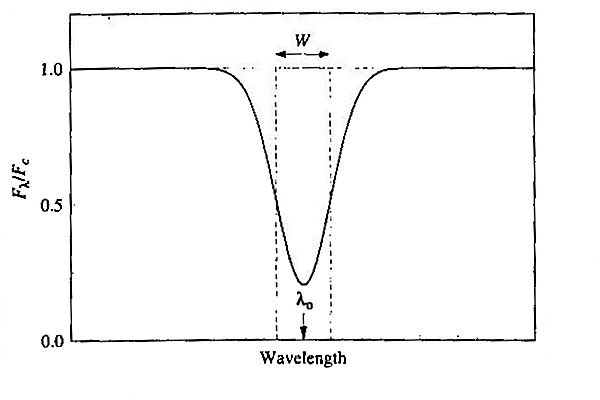
\includegraphics[width=5.0in]{CarrollEquiv}
\caption{%
Example of a spectral absorption line at $\lambda=\lambda_0$,
indicating the equivalent width $W$ of the
feature (Carroll \& Ostlie 1996). }%
\label{cha:InfraredDataReductionTechniques:sec:Spectroscopy:subsec:EquivalentWidth:fig:CarrollEquiv}
\end{center}
\end{figure}
%%%%%%%%%%%%%%%%%%%%%%%%%%%%%%%%%%%%%%%%%%%%%%%%%%%%%%%%%%%%%%%%%%

\nocite{CarrollOstlie:1996}

%%%%%%%%%%%%%%%%%%%%%%%%%%%%% Radial Velocity %%%%%%%%%%%%%%%%%%%%

\subsection{The Radial Velocity of the Secondary Star}
\label{cha:InfraredDataReductionTechniques:sec:Spectroscopy:subsec:RadialVelocity}

We used spectroscopy in order to verify that the disk in our target system was not contaminating the light curve of the binary. We also measured the \textbf{radial velocity} of the secondary star, so as to confirm that our spectra were consistent with past observations. This was especially necessary as these were the first high signal-to-noise $K$--band spectra of a black hole X--ray
transient system. 

\vspace{\myparskip}

The radial velocity of the secondary star in a
binary system may be calculated from:
\begin{eqnarray}
\label{cha:InfraredDataReductionTechniques:sec:Spectroscopy:subsec:RadialVelocity:eqn:Vr}
v_r = \gamma + K_2 \sin{(2\pi\phi)},
\end{eqnarray}
where $\gamma$ is the systematic velocity of the binary system, and
$\phi$ is the orbital phase of the binary.  

\vspace{\myparskip}

The radial velocity can be measured from the
Doppler shift of the observed wavelengths of the spectral features
in the spectrum of the star, which is a result of the motion of the star relative to the observer along their line of sight. This shift is given by:%
\begin{eqnarray}
\label{cha:InfraredDataReductionTechniques:sec:Spectroscopy:subsec:RadialVelocity:eqn:shift}
\Delta\lambda 	& = & \lambda_{\mathrm{obs}} - \lambda,\\
       		& = & \frac{v_r \lambda}{c},
\end{eqnarray}
where $\lambda$ and $\lambda_{\mathrm{obs}}$ are the rest and
observed wavelengths, respectively, of the spectral
feature. Therefore, if we know $\Delta\lambda$, we can also calculate the
radial velocity from:%
\begin{eqnarray}
\label{cha:InfraredDataReductionTechniques:sec:Spectroscopy:subsec:RadialVelocity:eqn:vr2}
v_r = \frac{\Delta\lambda}{\lambda} c.
\end{eqnarray}

\vspace{\myparskip}

We compared the predicted radial velocity of our target star
(calculated using the published spectroscopic ephemeris) with that
determined from the $\Delta\lambda$ measured from the spectrum of the star, to ensure that our result agreed with prior observations of \groj. %

%%%%%%%%%%%%%%%%%%%%%%%%%%%%% Infrared Astronomy %%%%%%%%%%%%%%%%%%%%

\section{Advantages of IR Observations of \groj}
\label{cha:InfraredDataReductionTechniques:sec:InfraredAstronomy}

This thesis is concerned with the infrared observations of the X--ray binary\\%
% WHITE SPACE %
\groj. Although X--ray binaries emit energy primarily as X--rays, our
observations of \groj\ were made at infrared wavelengths,
(the $J$--, $K$-- and $K_{s}$--bands). This section explains the
advantages for doing so, as well as the drawbacks of infrared
observations. %

%%%%%%%%%%%%%%%%%%%%%%%%%%%%% Dominance of Secondary %%%%%%%%%%%%%%%%%%%%

\subsubsection{Dominance of Secondary}
\label{cha:InfraredDataReductionTechniques:sec:InfraredAstronomy:subsubsec:DominanceOfSecondary}


A luminous accretion disk in a binary system will be bluer than the secondary star, and should contribute less in the infrared than in the optical. Hence this intrinsic emission from the secondary star should dominate in the infrared, and this will allow a better estimate of the brightness of the secondary to be made. This increases the likelihood of tightly constraining the mass ratio, inclination and black hole mass through infrared observations. %

%%%%%%%%%%%%%%%%%%%%%%%%%%%%% Infrared Spectroscopy %%%%%%%%%%%%%%%%%%%%

\subsubsection{Disk Contamination and Infrared Spectroscopy}
\label{cha:InfraredDataReductionTechniques:sec:InfraredAstronomy:subsubsec:InfraredSpectroscopy}

If we ignore the accretion disk contribution for a given binary
system, we cannot be certain that we are not underestimating the
orbital inclination for that system, or that our derived stellar masses are valid estimates. %
Although the quiescent infrared disk contribution is often
assumed be negligible (see, for example, %
\citeNP{ShahbazNaylorCharles:1994}%
), it is possible that the disk can in fact be a
strong source of infrared radiation. 
Infrared spectroscopy can be used to constrain the level of 
accretion disk contamination in the infrared during
quiescence. %

%%%%%%%%%%%%%%%%%%%%%%%%%%%%% Interstellar Extinction %%%%%%%%%%%%%%%%%%%%

\subsubsection{Interstellar Extinction}
\label{cha:InfraredDataReductionTechniques:sec:InfraredAstronomy:subsubsec:InterstellarExtinction}

In general, the $K$--band interstellar extinction, $A_K$, is nine times smaller
 than visual band extinction, $A_V$ ($A_K \sim 0.114\ A_V$: %
\citeNP{CardelliClaytonMathis:1989}). Therefore, the interstellar medium absorbs less infrared radiation
than optical. Hence any attempt to locate a faint distant object may be more
successful if the observations are made in the infrared. %

\vspace{\myparskip}

More specifically, we will later show that our target system \groj\ has a high visual extinction of $A_{V} =4.0\pm0.3$\,mag, but a low infrared extinction $A_{K} = 0.42\pm0.04$\,mag (see \S~\vref{cha:lightcurve:sec:Photometry:subsec:DereddenedMagnitude}). This system is therefore
less obscured in the infrared, which improves the quality of images taken at these wavelengths. %

%%%%%%%%%%%%%%%%%%%%%%%%%%%%% Improved Resolution %%%%%%%%%%%%%%%%%%%%

\subsubsection{Improved Spatial Resolution}
\label{cha:InfraredDataReductionTechniques:sec:InfraredAstronomy:subsubsec:ImprovedResolution}

More generally, the resolution of an observation specifies the minimum angular
separation required between two stars for the pair to be
distinguishable. At wavelengths less than or equal to infrared wavelengths
(1.0--2.4$\,\mu \mathrm{m}$), and for 1-m or larger telescopes, this
resolution is determined mainly by the effect of turbulence in the
atmosphere (see, e.g., %
\citeNP{Schroeder:1987:Resolution}%
\ for details). In this regime, there is an improvement in resolution
with increasing wavelength, as the longer wavelengths are less
refracted by the atmosphere than the shorter wavelengths. Therefore,
the infrared offers better quality images than the optical
(400--700\,nm). %

%%%%%%%%%%%%%%%%%%%%%%%%%%%%% Disadvantages %%%%%%%%%%%%%%%%%%%%

\subsubsection{Disadvantages}
\label{cha:InfraredDataReductionTechniques:sec:InfraredAstronomy:subsubsec:Disadvantages}

The main disadvantage of infrared photometry is that the background
is much higher relative to that at, for example, optical
wavelengths. Before any meaningful analysis can be made, the thermal
background from the atmosphere and even the instruments and the telescope used to
make the observations must be accounted for.

\vspace{\myparskip}

Also, in order to obtain useful infrared spectra, the
atmospheric absorption or \textbf{telluric} features caused by the presence of oxygen and water vapour in the
Earth's atmosphere must be accurately subtracted. The OH lines in the
atmosphere would otherwise dominate the spectra. This increases the
difficulty of data reduction in comparison to optical spectroscopy. %

\vspace{\myparskip}

Once we make our infrared observations of a target star, we have to perform either photometric or spectroscopic data reduction to obtain information about our system of interest. %

%%%%%%%%%%%%%%%%%%%%%%%%%%%%% Photometric Data Reduction %%%%%%%%%%%%%%%%%%%%

\section{Reduction of Infrared Photometric Data}
\label{cha:InfraredDataReductionTechniques:sec:Photometry}

We can employ photometry to determine the brightness of a binary star
from infrared observations of that star. The raw images of the star are first processed to improve their quality. This is known as \textbf{Image Reduction}. Then we obtain the magnitude of the target star relative to
several comparison stars in each processed image. The images are
calibrated to obtain the apparent magnitudes of the chosen stars in
the sky. Finally, the absolute magnitude of the target star is
calculated, taking its distance and interstellar extinction into
account. 


%%%%%%%%%%%%%%%%%%%%%%%%%%%%% IRAF and DS9 %%%%%%%%%%%%%%%%%%%%

\subsection{\iraf\ and \texttt{DS9}}
\label{cha:InfraredDataReductionTechniques:sec:Photometry:subsec:IRAFAndDS9}

Much of the image reduction and data analysis performed can be done using
the \textbf{Image Reduction and Analysis Facility (IRAF)} package
(v 2.11.3), a product of the U.S. National Optical Astronomy Observatories
(NOAO). The \iraf\ tasks and packages that we run are denoted in this
section by \texttt{typewriter} font. The task parameters and their
values are written using the \textit{italic} font. %

\vspace{\myparskip}

Occasionally throughout the reduction and analysis, it is necessary
to view and interact with the images. Our image viewer is 
\textbf{SAOIMAGE DS9} (v 2.1b4), written by the Smithsonian
Astrophysical Observatory Research and Development Group. %


%%%%%%%%%%%%%%%%%%%%%%%%%%%%% Image Reduction %%%%%%%%%%%%%%%%%%%%

\subsection{Image Reduction}
\label{cha:InfraredDataReductionTechniques:sec:Photometry:subsec:ImageReduction}

Our observations involve centering the telescope on the target and
then obtaining a group of images -- normally nine images are obtained
per group. The images form a grid, with each image offset by
approximately 10\% of the field of view from a common point in the
sky. %

\vspace{\myparskip}

For each grid of $K$-- or $J$--band images, the following procedure is
performed to produce a high-quality image from which the magnitude of
the star can be determined. (More comprehensive details of elements of the photometric image
reduction procedure may be found in \S~%
\vref{cha:IRAF:sec:Photometry}.) %

%%%%%%%%%%%%%%%%%%%%%%%%%%%%% Background Subtraction %%%%%%%%%%%%%%%%%%%%

\subsection{Background Subtraction}
\label{cha:InfraredDataReductionTechniques:sec:Photometry:subsec:BackgroundSubtraction}

As mentioned on page~%
\pageref{cha:InfraredDataReductionTechniques:sec:InfraredAstronomy:subsubsec:Disadvantages},%
\ the use of infrared observations suffers from the disadvantage that
the background level is higher than for observations obtained at, for
example, optical wavelengths. Unprocessed source images therefore
reveal little, as most of the stars are obscured by this
background. Nevertheless, it is possible to estimate the background
and subtract it from the raw images, resulting in superior data. %

\vspace{\myparskip}

An image is created from the grid of images using the
\texttt{imcombine} command. The parameter \textit{combine} is set to
\textit{median}, that is, the value of each pixel is taken to be the
median value of that pixel over the images in the grid. As long as the
pixel detected flux from a star in less than half of the images (i.e.,
the observed field was not crowded), this median value should be an
approximation of the background level at that pixel. This assumes that
the background did not vary as the telescope pointing changed,
and that it was constant over the time of the observation. Since the
cloud cover, wind speed and atmospheric temperature are often more or less constant
for this period of time (about 30 mins), the approximation
is normally accurate. The median pixel file, called the
\textbf{background image}, is therefore used to subtract the background from the original images
using \texttt{imarith}. A new background file is created for each
grid of images. %

%%%%%%%%%%%%%%%%%%%%%%%%%%%%% Flatfield %%%%%%%%%%%%%%%%%%%%

\subsection{Flatfield}
\label{cha:InfraredDataReductionTechniques:sec:Photometry:subsec:Flatfield}

Having subtracted the background image, we then take into
account the intrinsic
pixel to pixel variations for the observed wavelengths. To do this, a
\textbf{flatfield image}, which represents this variability, is
created using one of the 
following methods. %

\vspace{\myparskip}

The first method is to make a \textbf{dome flat}%
. During the observation run, an image of an illuminated spot inside the closed observatory dome
is obtained, as well as an exposure of the spot without
illumination but with the same integration time. This procedure is repeated several times throughout the period of observations. The
two sets of illuminated and non-illuminated images are then
\texttt{imcombine}d (with \textit{combine}=\textit{average})
separately so as to obtain an averaged illuminated and non-illuminated
image, respectively. Using \texttt{imarith}, the non-illuminated image
is subtracted from the illuminated image. The resultant subtracted
image is divided by its median pixel value (obtained from
\texttt{imstat}) to obtain the flatfield image. The background
subtracted images are then divided by the flatfield. %

\vspace{\myparskip}

An alternative method is \textbf{median combination}, which can be
used if no dome flats are obtained during the observation run. First, all the images obtained during the run are \texttt{imcombine}d using the
median value for each pixel. Once more, it is assumed that in a
sparse field, this median value represents the background. Second,
the median pixel value of the median image is obtained from
\texttt{imstat}, and the image is divided by this value (again using
\texttt{imarith}). Third, the resultant image is taken as an
approximation of the relative response of each pixel, and the
subtracted images are divided by this flatfield. %

%%%%%%%%%%%%%%%%%%%%%%%%%%%%% Bad Pixels %%%%%%%%%%%%%%%%%%%%

\subsection{Bad Pixels}
\label{cha:InfraredDataReductionTechniques:sec:Photometry:subsec:BadPixels}

Some of the pixels in a detector may not respond properly to radiation
of any wavelength, and record an excessively high or low value for the
incident flux. These pixels, known as \textbf{bad pixels}, %
should be disregarded when viewing the background subtracted,
flatfielded images. This is done automatically by creating a
\textbf{bad pixel map}. %

\vspace{\myparskip}

Firstly, the raw images are median combined and the resultant image
divided by its overall median pixel value, in a similar manner to the 
median combined flatfield method discussed above. Secondly, the value of each pixel in the divided image is written to a text file using the \texttt{listpixel} command. Since the average
value of a pixel in the divided image should have been approximately
1, the pixels that registered a value of below 0.75 or above 1.25 are
chosen as the bad pixels for the detector. These pixels are used by
the \texttt{badpiximage} command to create a bad pixel map. %

%%%%%%%%%%%%%%%%%%%%%%%%%%%%% Combining the Grid %%%%%%%%%%%%%%%%%%%%

\subsection{Combining the Grid}
\label{cha:InfraredDataReductionTechniques:sec:Photometry:subsec:CombiningTheGrid}

We can now combine all the processed images to produce high quality images of our target.%

\vspace{\myparskip}

If all the images taken are of the same field of view,
a common point in the images can be selected, which is in the
central region of each image. The background subtracted and
flatfielded images are then shifted using the
\texttt{imshift} command, so that this common point is at the same
coordinates in each image. The corresponding bad pixel map previously
created is also shifted for each image, so as to account for the
relocation of the bad pixels in that image. %

\vspace{\myparskip}

Using \texttt{imcombine}, each grid of frames are average
combined. The combined images are then visually examined, and those of
unacceptable quality are discarded. %

%%%%%%%%%%%%%%%%%%%%%%%%%%%%% Relative Photometry %%%%%%%%%%%%%%%%%%%%

\subsection{Relative Photometry}
\label{cha:InfraredDataReductionTechniques:sec:Photometry:subsec:RelativePhotometry}

Once processed images have been acquired, it is possible to determine
the brightness of the stars in the field of view. For
the purposes of studying the variability of systems like \groj,
we need only the brightness of the system relative to a star of
constant brightness. Nevertheless, in order to compare our
observations with previous ones, we also require a calibrated measure
of the brightness of the system. % 

\vspace{\myparskip}

\textbf{Relative} or \textbf{differential photometry} %
is the calculation of the magnitude of one star relative to
another. This technique is useful because, although the observed magnitudes of
two constant, neighbouring stars may appear to vary in time (due to
changing atmospheric conditions), the magnitude of one relative to the
other should not. Therefore, if we determine the magnitude of our
target star relative to a constant star in the field of view, we can
attribute any variation in this value to the changing intrinsic magnitude of our star. %

\vspace{\myparskip}

Relative photometry can be carried out using the \iraf\ adaptation of the \texttt{DAOPHOT} package for crowded field stellar photometry%
\ \cite{Stetson:1987}. %
(See \S~%
\vref{cha:IRAF:sec:Photometry:subsec:DAOPHOT}%
\ for details of this procedure.) %
Firstly, we select a constant star (which we denote as our \textbf{comparison star})%
\label{cha:InfraredDataReductionTechniques:sec:Photometry:subsec:RelativePhotometry:topic:comparison}%
\ of comparable brightness to our target star, and several bright constant stars in the field of view (our \textbf{reference stars}). These stars, together with our target star, are denoted as our stars of
interest. Secondly, \texttt{DAOPHOT} is run to remove near neighbours of the selected
stars. Several isolated faint stars in the field of view are chosen
as model stars, and are used by \texttt{DAOPHOT} to create a
\textbf{point spread function (PSF)} model. 
This PSF model is then fitted to all our stars of interest and the instrumental magnitudes are obtained from \texttt{allstar}. The magnitudes of the reference stars are averaged, and this value
subtracted from the magnitude of the target star and the comparison star.  The
Julian Date of each observation is determined from the Universal Date
and Time. The two relative magnitudes are plotted against the Julian Dates of
the observations to obtain the light curves of the target and
comparison star. The light curve of the comparison star generated in this way can be used as a measure of the error in our target star light curve. If we know the orbital ephemeris of the target star, we can then fold the light curve of the target star to search for systematic variations as a function of orbital phases. %

\vspace{\myparskip}

Finally, in order to estimate the average magnitude of the possibly
variable star, we obtain the \textbf{phase averaged relative
magnitude}:%
\label{cha:InfraredDataReductionTechniques:sec:Photometry:subsec:RelativePhotometry:topic:parm}%
\ we average the values for the magnitude of our target star
relative to one particular reference star. 

%%%%%%%%%%%%%%%%%%%%%%%%%%%%% Aperture Photometry and Photometric Calibration %%%%%%%%%%%%%%%%%%%%

\subsection{Aperture Photometry and Photometric Calibration}
\label{cha:InfraredDataReductionTechniques:sec:Photometry:subsec:AperturePhotometry}

Although we now have the magnitude of our star relative to a constant
star, we don't know the actual magnitude of the star itself. This we
estimate by first manually determining the instrumental magnitude of the
star using \textbf{aperture photometry}, and then calculating the apparent magnitude of the system. %

\vspace{\myparskip}

First, we obtain the counts per second ($f_{10}$) detected by our
telescope from a star of known magnitude, say magnitude 10. We then 
\begin{inparaenum}[(i)] 
\item determine the number of counts per second measured from this comparison star,
\item correcte this for atmospheric extinction, and
\item comparee this to $f_{10}$, to obtain the apparent magnitude of the comparison star. 
\end{inparaenum}

\vspace{\myparskip}

This process is performed for both the $J$-- and $K_{s}$--band observations. This magnitude is then used to calibrate the (phase averaged) magnitude of our target star, allowing us to finally calculate the phase averaged $K_{s}$-- and $J$--band apparent magnitudes of our target star. %

%%%%%%%%%%%%%%%%%%%%%%%%%%%%% Dereddened and Absolute Magnitudes %%%%%%%%%%%%%%%%%%%%

\subsection{Dereddened and Absolute Magnitudes}
\label{cha:InfraredDataReductionTechniques:sec:Photometry:subsec:DereddenedMagnitude}

We can now calculate the \textbf{dereddened magnitude} of the star by
determining the necessary corrections to account for interstellar
extinction (see \S~%
\vref{cha:InfraredDataReductionTechniques:sec:MagnitudeScale:subsec:InterstellarExtinction}%
). %

\vspace{\myparskip}

If we know the value of $E_{B-V}$, we can calculate the $K$--band extinction from Equation~%
\vref{cha:InfraredDataReductionTechniques:sec:MagnitudeScale:subsec:InterstellarExtinctioneqn:CardelliAK}%
: %
\begin{eqnarray} 
\label{cha:InfraredDataReductionTechniques:sec:Photometry:subsec:DereddenedMagnitude:eqn:CardelliAK}
A_{K}    & = & 0.114 \times R_V \times E_{B-V}, \nonumber
\end{eqnarray} 
and similarly for the $J$--band extinction. Then, the dereddened
magnitude ($K_{0}$) of our target star in the $K$--band can be found via:
\begin{eqnarray} 
\label{cha:InfraredDataReductionTechniques:sec:Photometry:subsec:DereddenedMagnitude:eqn:K0}
K_0 & = & \mathrm{apparent\ } K_{s} \mathrm{\ magnitude} - A_K,
\end{eqnarray} 
and similarly for the $J$--band. %

\vspace{\myparskip}

The last step in the photometric data reduction is to calculate the
absolute magnitude of the target star. Assuming we know the distance to the star, the $J$ and $K$ absolute magnitudes of the star can then be
calculated using Equations~%
\ref{cha:InfraredDataReductionTechniques:sec:MagnitudeScale:subsec:AbsoluteMagnitude:eqn:AbsMagK}%
~and~%
\ref{cha:InfraredDataReductionTechniques:sec:MagnitudeScale:subsec:AbsoluteMagnitude:eqn:AbsMagJ}.%

%%%%%%%%%%%%%%%%%%%%%%%%%%%%% Spectroscopic Data Reduction %%%%%%%%%%%%%%%%%%%%

\section{Reduction of Infrared Spectroscopic Data}
\label{cha:InfraredDataReductionTechniques:sec:SpectroscopyData}

Just as we need to correct our photometric data for the background and
detector pixel variations, we need to process our spectra to 
\begin{inparaenum}[(i)] 
\item account for the background,
\item apply a dispersion correction, and 
\item remove telluric features.
\end{inparaenum}
The corrected spectra can then be averaged to obtain our final target spectrum. %
(Further details on the steps in the procedure for the reduction of the
spectroscopic data can be found in \S~%
\vref{cha:IRAF:sec:Spectroscopy}.)%

%%%%%%%%%%%%%%%%%%%%%%%%%%%%% Background Subtraction %%%%%%%%%%%%%%%%%%%%

\subsection{Background Subtraction}
\label{cha:InfraredDataReductionTechniques:sec:SpectroscopyData:subsec:BackgroundSubtraction}

The first step in producing processed spectra is to subtract the background from
each of the observations. We can do this by selecting two images of our
star, and subtracting one from the other and vice versa. In this way,
we obtain two subtracted images of the star. Since the object appears
at different places on the slit in the two original images, there is
no overlap of the object spectrum between the images. This subtraction
is done for the spectra of each star. %

%%%%%%%%%%%%%%%%%%%%%%%%%%%%% Spectra Extraction %%%%%%%%%%%%%%%%%%%%

\subsection{Spectra Extraction}
\label{cha:InfraredDataReductionTechniques:sec:SpectroscopyData:subsec:SpectraExtraction}

The background subtracted images are then processed using
\texttt{apall} to obtain 1-D spectra for each star. An Argon arc lamp spectrum is also extracted for
each star, using the trace for the star to trace the corresponding arc. %

%%%%%%%%%%%%%%%%%%%%%%%%%%%%% Wavelength Calibration %%%%%%%%%%%%%%%%%%%%

\subsection{Wavelength Calibration}
\label{cha:InfraredDataReductionTechniques:sec:SpectroscopyData:subsec:WavelengthCalibration}

The extracted spectra are plotted to display the flux from the star
detected by each pixel of the detector. However, in order to compare
the spectra with previous observations, we need to determine the
flux as a function of wavelength. This calibration of the spectra is
done by using our extracted arc spectra as a reference. The known
wavelength of each Ar feature is compared to the pixel value at which
the feature is observed in the arc spectra. The \texttt{identify} and \texttt{reidentify} tasks are
then run to calculate a dispersion correction to obtain a
corresponding wavelength for each pixel. This dispersion correction is then applied by \texttt{dispcor} to the extracted spectra. %

%%%%%%%%%%%%%%%%%%%%%%%%%%%%% Normalisation %%%%%%%%%%%%%%%%%%%%

\subsection{Normalisation}
\label{cha:InfraredDataReductionTechniques:sec:SpectroscopyData:subsec:Normalisation}

To study the absorption and emission features in the spectra, it is useful to normalise the spectra to the continuum flux. We normalise our
wavelength-callibrated spectra by using the task \texttt{continuum} to
fit the continuum of each spectrum to a spline of order 2. %


%%%%%%%%%%%%%%%%%%%%%%%%%%%%% Telluric Features %%%%%%%%%%%%%%%%%%%%

\subsection{Removing Telluric Features}
\label{cha:InfraredDataReductionTechniques:sec:SpectroscopyData:subsec:TelluricFeatures}

Next, the telluric
features present in raw spectra must be removed. This is especially
important in the infrared, where atmospheric features can dominate the
spectra. %

\vspace{\myparskip}

The telluric features can be accounted for by dividing the
target star spectra by the spectrum of a nearby star. This method assumes that both stars are affected in the same way by the telluric features, and hence dividing one by the other should, in theory, cancel this effect. This method has a
systematic error, in that the absorption features present in the nearby
star will be seen as emission features in the divided spectra. This
effect can be minimised by choosing a star with few prominent spectral
features. %

\vspace{\myparskip}

An A0-type star may be chosen as the comparison star because of the
large effective temperature of stars of this classification, which
results in a spectrum with only one prominent feature in the
$K$--band.  This is the neutral hydrogen absorption line \mbox{H I
(4--7)} at $\lambda=21\,655$\,\AA, known as the Brackett-$\gamma$
(Br-$\gamma$) absorption feature. We then assume that the other
features in our spectra of our comparison star are telluric. This feature is masked and the resulting A0 spectrum is divided into the target spectrum to remove the telluric features. %

%%%%%%%%%%%%%%%%%%%%%%%%%%%%% Combining the Spectra  %%%%%%%%%%%%%%%%%%%%

\subsection{Combining the Spectra}
\label{cha:InfraredDataReductionTechniques:sec:SpectroscopyData:subsec:CombiningTheSpectra}

The two target star spectra, corrected for telluric features using the comparison
star, are combined using \texttt{scombine} (\textit{combine} set to
\textit{average}). The resultant spectrum is smoothed using
\texttt{splot}, with a bin size of 3, to obtain the final spectrum. %

%%%%%%%%%%%%%%%%%%%%%%%%%%%%% Our System of Interest %%%%%%%%%%%%%%%%%%%%

\section{Our System of Interest}
\label{cha:InfraredDataReductionTechniques:sec:SystemOfInterest}

We now consider \groj\ in detail and present the reasons for studying
this transient. We will then apply the data reduction techniques we have outlined to this system, and attempt to obtain an estimate for the mass of the primary star within this binary
system.

%%%%%%%%%%%%%%%%%%%%%%%%%%%%% End of Chapter %%%%%%%%%%%%%%%%%%%%


% chktex-file 44
%%%%%%%%%%%%%%%%%%%%%%%%%%%%% GRO J1655-40 %%%%%%%%%%%%%%%%%%%%
\chapter{\groj}\label{cha:GROJ1655-40}

In this chapter, we first detail the system properties of \groj, with
emphasis on the accretion disk surrounding the primary star. We list
the observations we made of this SXT, and also elucidate the general reasons for studying this
system. %

\vspace{\myparskip}

Our specific reason for studying \groj\ is to obtain an estimate of
the mass of the black hole which this system is thought to harbour. If
we assume that the accretion disk contributes little to the total flux
from the system, we can then constrain the mass ratio $q$ (and hence the primary mass $M_{X}$) and the inclination $i$  from the ellipsoidal modulation of the binary and the radial velocity curve. %

\vspace{\myparskip}

We will therefore later explain how we applied infrared photometric techniques to obtain the light curve of \groj\ during the period of our observations, and show how we determined the mass of the black hole from the light curve, before discussing whether our assumption of negligible disk
contamination is valid.

%%%%%%%%%%%%%%%%%%%%%%%%%%%%% Introduction to GRO J1655-40 %%%%%%%%%%%%%%%%%%%%

\section{Introduction to \groj}\label{cha:GROJ1655-40:sec:IntroductionToJ1655}

In July 1994, \mbox{GRO J1655--40}\footnote{\label{cha:GROJ1655-40:sec:IntroductionToJ1655:foot:SIMBAD}
The SIMBAD identifier of \groj\ is V* V1033 Sco. It is also
referred to as \textbf{\nova\ (\mbox{Nova Sco 1994})}.%
}%
\ was observed for the first time by the Burst and
Transient Source Experiment (BATSE) onboard the Compton Gamma Ray
Observatory (CGRO) (Zhang et~al.\ \citeyearNP{Zhang_et_al.:1994}). %
Four outbursts in total were observed in the first five months after
its discovery (Harmon et~al.\ \citeyearNP{Harmon_et_al.:1995}).%
\ The optical counterpart of this system was identified in 1995 by
Bailyn et~al.\ \citeyear{BailynOroszGirad_et_al.:1995}%
, the mass function derived by several observers (e.g.,
\citeNP{OroszBailyn:1997}) for the primary star in \groj\ indicated
that this system might contain a black hole. %

%%%%%%%%%%%%%%%%%%%%%%%%%%%%% Properties of J1655 %%%%%%%%%%%%%%%%%%%%

\subsection{General Properties and Special Characteristics}\label{cha:GROJ1655-40:sec:IntroductionToJ1655:subsec:PropertiesOfJ1655}

%%%%%%%%%%%%%%%%%%%%%%%%%%%%% System Properties %%%%%%%%%%%%%%%%%%%%

\subsubsection{System Properties}\label{cha:GROJ1655-40:sec:IntroductionToJ1655:subsec:PropertiesOfJ1655:subsubsec:SystemProperties}

\groj\ lies approximately 3.2 kiloparsecs (kpc) away %
\cite{HjellmingRupen:1995}. Hynes et~al.\ %
\citeyear{Hynes_et_al.:1998}%
\ derived a reddening $E_{B-V}$ of $1.2\pm0.1$\,mag for \groj, from which
they calculate a hydrogen column density of $N_H
\sim5\times10^{21}\,\mathrm{cm}^{-2}$. From these values, the
quiescent bolometric luminosity of \groj\ can be determined to be
approximately $41\,\mathrm{L}\sun$ (see, e.g., %
van~der~Hooft et~al.\ %
\citeyearNP{VanDerHooft_et_al.:1998}).%
\ The quiescent $V$--band magnitude of \groj\ is approximately 17.1
mag %
\cite{GreeneBailynOrosz:2001}, %
and the system becomes as bright as 16.2 mag in the $V$--band during
outburst %
\cite{BailynOroszMcClintockRemillard:1995}. %

\vspace{\myparskip}

The times of the inferior conjunction of the primary are described by the
following photometric ephemeris (van~der~Hooft et~al.\ %
\citeyearNP{VanDerHooft_et_al.:1998})%
, given in MJD%
\footnote{\label{cha:GROJ1655-40:sec:IntroductionToJ1655:subsec:PropertiesOfJ1655:subsubsec:SystemProperties:foot:mjd}%
The \textbf{Modified Julian Date (MJD)} is defined to be the Julian
Date (JD) minus 2400000.5.} %
:
\begin{eqnarray}\label{cha:GROJ1655-40:sec:IntroductionToJ1655:subsec:PropertiesOfJ1655:subsubsec:SystemProperties:eqn:Ephemeris}
\nonumber T_{\mathrm{min}}\ (\mathrm{MJD}) & = &T_0 + P \times N, \\
 & = & 49838.4198(52) + 2.62168(14) \times N,
\end{eqnarray}
where $T_0$ is the time of mid--eclipse, $P$ is the orbital period and $N$
denotes the number of orbital cycles. %

\vspace{\myparskip}

The most recent values for the mass ratio and
inclination of \groj\ are those predicted by %
\citeN{BeerPodsiadlowski:2001}. They derived values of $q=3.9\pm0.6$ and $i=68 \fdg 65 \pm
1 \fdg 5$. Using the mass function of \citeN{Shahbaz_et_al.:1999}, %
$f(M_X) = 2.73\pm0.09\,M\sun$, they determined that
\groj\ consists of a $5.4\pm0.3$\,M\sun\ black hole primary and a
$1.45\pm0.35$\,M\sun\ secondary. The secondary is a giant (or subgiant) of spectra type F5--G0%
, and orbits at a distance of approximately 16.6\,R\sun\ from the primary. %

%%%%%%%%%%%%%%%%%%%%%%%%%%%%% Eccentricities %%%%%%%%%%%%%%%%%%%%

\subsubsection{Anomalies}\label{cha:GROJ1655-40:sec:IntroductionToJ1655:subsec:PropertiesOfJ1655:subsubsec:Eccentricities}

\groj\ displays several atypical characteristics:

\begin{itemize}

\item %
\groj\ is optically the brightest in quiescence of all SXTs. %
The secondary dominates in quiescence to an unusually large extent,
due its relatively luminous F/G star nature.
The light curves of \groj\ are therefore unusually smooth and
symmetrical when compared to those of other black hole binaries, and
so the measurements of the mass ratio and inclination of this system
should therefore be atypically precise. %

\item
\groj\ is one of three known Galactic X--ray sources with apparently superluminal
jets -- another being GRS 1915+105 -- (see Tavani et~al.\ %
\citeyearNP{Tavani_et_al.:1996} %
and references therein), and is the only such source to be identified
optically. \groj\ is also less obscured by dust than \mbox{GRS 1915+105}, and is hence more easily studied.
The jets were discovered by Tingay et~al.\ %
\citeyear{Tingay_et_al.:1995} %
and were shown to have actual speeds of $0.92 \pm 0.02\,c$ by %
\citeN{HjellmingRupen:1995}. %

Most other SXTs have shorter periods and smaller accretion disks %
(Hynes et~al.\ %
\citeyearNP{Hynes_et_al.:1998}).%

\item Kolb et~al.\ %
\citeyear{Kolb_et_al.:1997}%
\ suggested that \groj\ is in a different evolutionary state to other
SXTs. %
Although the secondary stars in SXTs are evolved, the secondary in
\groj\ is an extreme case, and has almost become a giant. %

\item
\groj\ has an unusually high accretion rate ($\dot{M}_{2}$), which
is close to its critical value ($\dot{M}_{\mathrm{crit}}$): these
rates were calculated by %
\citeN{OroszBailyn:1997}%
\ to be $3.4\times10^{-9}\,\mathrm{M}\sun\,\mathrm{yr}^{-1}$ and
$1.1\times10^{-8}\,\mathrm{M}\sun\,\mathrm{yr}^{-1}$,
respectively. This implies that \groj\ is likely to have frequent
X--ray outbursts. %



\item \groj\ is the only SXT to show evidence of eclipses, as observed by
Bailyn et al.\ %
\citeyear{BailynOroszGirad_et_al.:1995}%
\ at optical wavelengths. These eclipses are of the
accretion disk and suggest that $i$ is large. However, no eclipses are
observed in the X--ray, which implies that the compact object is not
eclipsed by the secondary star, and negates the possibility that
$i\sim90\degr$ %
\cite{OroszBailyn:1997}%
. Nevertheless, Zhang et al.\ %
\citeyear{Zhang_et_al.:1997} %
noted that the high inclination angle of \groj\ is the largest amongst
all well-known Galactic black hole binaries. %

\item
The systematic velocity of \groj, $\gamma =
-142.4\pm1.6\,\mathrm{km\,s^{-1}}$ %
\cite{OroszBailyn:1997}%
, is atypically high for a LMXB containing a black hole. This value is
more suggestive of a neutron star binary. %
Brandt et~al.\ %
\citeyear{Brandt_et_al.:1995}%
\ suggested that the progenitor of the primary star in \groj\ did not
collapse directly into a black hole. Rather, it was formed when a
neutron star evolved into a black hole due to the accretion of
additional mass. This evolutionary process would account for the
abnormal $\gamma$--velocity. Mirabel et~al.\ %
\citeyear{Mirabel_et_al.:2002:unchecked}%
\ confirmed that both the systematic velocity and the high
galactocentric eccentricity ($e=0.34\pm0.05$) of this system could be explained by a
natal explosion. %

\end{itemize}

%%%%%%%%%%%%%%%%%%%%%%%%%%%%% Reasons to Study J1655 %%%%%%%%%%%%%%%%%%%%

\subsection{Reasons to Study \groj}\label{cha:GROJ1655-40:sec:IntroductionToJ1655:subsec:ReasonsToStudyJ1655}

If we can assume a negligible disk contribution, the unique
ellipsoidal variations and eclipses of \groj\ should allow us to constrain
the mass ratio and inclination considerably. This will lead to a unprecedented precision in the measurement of the
mass ratio and orbital inclination -- see, for example, %
\citeN{OroszBailyn:1997}.%
\ The high precision in $q$ and $i$ in return should enable a similarly precise value
for the mass of the primary to be determined, strengthening the
evidence for the black hole nature of this star. %

\vspace{\myparskip}

\groj\ is also important due to its superluminal jet nature. The study of Galactic superluminal X--ray sources is important as it
may lead to a better understanding of \textbf{Active Galactic Nuclei
(AGN)}. These show similar jet geometry to these Galactic sources,
possibly due to comparable conditions of accretion. AGN are thought to
be powered by massive ($\lsim 10^{10}$\,M\sun) black holes and may be the
high-luminosity counterparts to sources such as \groj. %

\vspace{\myparskip}

Finally, further study of the eclipses in \groj\ may lead to information on the
structure of the disk in this system. \groj\ therefore could be the best X--ray binary with which to test
various models of X--ray production and jet formation in the search for
a better understanding of AGN. %

%%%%%%%%%%%%%%%%%%%%%%%%%%%%% The Accretion Disk in \groj %%%%%%%%%%%%%%%%%%%%

\subsection{The Accretion Disk Contribution in \groj}\label{cha:GROJ1655-40:sec:IntroductionToJ1655:subsec:TheAccretionDisk}

When modelling SXTs, it is often assumed that the accretion disk
contributes little light to the overall system flux during
quiescence (see page~%
\pageref{cha:InfraredDataReductionTechniques:sec:InfraredAstronomy:subsubsec:InfraredSpectroscopy}%
). Indeed, the spectral type of the secondary star in \groj\ is earlier than that in most other SXTs, implying that any small
contamination due to an accretion disk would be less significant than
in the other systems %
\cite{BeerPodsiadlowski:2001}%
. However, it is important to verify the above assumption for \groj, if the derived
system parameters are to be believed. %

\vspace{\myparskip}

Bailyn et~al.\ %
\citeyear{BailynJain_et_al.:1998}%
\ note that the disk in \groj\ is redder than the secondary during
quiescence. The unusually long period of this system implies that a
large disk can form, the outer parts of which will be cooler than in
other systems. These characteristics imply that there may
be more flux at the longer wavelengths, such as the infrared. This questions the validity of the
assumption that the quiescent disk contribution is negligible, even though there is no evidence of such a contribution from photometric measurements (see, for example, %
\citeNP{GreeneBailynOrosz:2001}%
). Therefore, the
disk contribution must be shown to be inconsequential using other
methods such as spectral analysis, if we are to accurately determine
the orbital inclination and mass ratio of \groj. %

%%%%%%%%%%%%%%%%%%%%%%%%%%%%% Observations of \groj\ %%%%%%%%%%%%%%%%%%%%

\section{Observations of \groj}\label{cha:GROJ1655-40:sec:ObservationsOfJ1655}

%%%%%%%%%%%%%%%%%%%%%%%%%%%%% The Observatories and the Instruments %%%%%%%%%%%%%%%%%%%%

\subsection{The Observatories and the Instruments}\label{cha:GROJ1655-40:sec:ObservationsOfJ1655:subsec:ObservatoriesAndInstruments}

%%%%%%%%%%%%%%%%%%%%%%%%%%%%% CIRIM %%%%%%%%%%%%%%%%%%%%

\subsubsection{The Cerro Tololo Infrared Imager at CTIO}\label{cha:GROJ1655-40:sec:ObservationsOfJ1655:subsubsec:CIRIM}

The 1995 and 1998 photometric observations of \groj\ were made using the
1.5m Ritchey-Chretien telescope at the \textbf{Cerro Tololo
Interamerican Observatory (CTIO)} located in Chile. The \textbf{Cerro
Tololo Infrared Imager (CIRIM)}%
\footnote{\label{cha:GROJ1655-40:sec:ObservationsOfJ1655:subsubsec:CIRIM:foot:CIRIM}
\url{http://www.ctio.noao.edu/instruments/ir_instruments/cirim/cirim.html}
}%
, a mercury-cadmium-telluride (HgCdTe) $256\times256$ NICMOS 3
array with a variable pixel scale, was the detector used. %

\vspace{\myparskip}

The $J$-- and $K_s$--band extinction coefficients, $k_J$ and $k_{K_{s}}$ (see
page~%
\pageref{cha:InfraredDataReductionTechniques:sec:MagnitudeScale:subsec:AtmosphericExtinction:topic:k}%
), at the observatory were previously measured
to be approximately $0.11$ mag/airmass and $0.064$ mag/airmass,
respectively %
\cite{Curran:2001}.

%%%%%%%%%%%%%%%%%%%%%%%%%%%%% NIRSPEC %%%%%%%%%%%%%%%%%%%%

\subsubsection{The Near Infrared Spectrometer at KECK}\label{cha:GROJ1655-40:sec:ObservationsOfJ1655:subsubsec:NIRSPEC}

Photometric and spectroscopic data for \groj\ were taken in 2000 at
the 10m Keck II telescope at the \textbf{W.M. Keck Observatory (KECK)}
in Mauna Kea, Hawaii.

\vspace{\myparskip}

The instrument selected for the spectroscopy was the \textbf{Near Infrared
Spectrometer} \textbf{(NIRSPEC)}%
\footnote{\label{cha:GROJ1655-40:sec:ObservationsOfJ1655:subsubsec:NIRSPEC:foot:NIRSPEC}
\url{http://www2.keck.hawaii.edu:3636/realpublic/inst/nirspec/nirspec.html}
}, %
a vacuum-cryogenic, high-resolution spectrograph for the Keck II
telescope. %

\vspace{\myparskip}

As part of NIRSPEC, the infrared \textbf{Slit-viewing Camera (S-CAM)}
operates over the wavelength region 0.95--2.5 microns. This HgCdTe
array has $256 \times 256$ pixels and a field of view of $46\arcsec
\times 46\arcsec$ (a pixel scale of $0.183\arcsec$/pixel). This
detector was used to obtain several images of \groj\ for use in
calibration. %

\vspace{\myparskip}

The extinction coefficient in the $K$--band, $k_K$, at the KECK observatory is
known to be $\sim 0.088$ mag/airmass %
\cite{Curran:2001}. %

%%%%%%%%%%%%%%%%%%%%%%%%%%%%% Details of the Observations %%%%%%%%%%%%%%%%%%%%

\subsection{Details of the Observations}\label{cha:GROJ1655-40:sec:ObservationsOfJ1655:subsec:DetailsOfTheObservations}

See Table~\vref{cha:GROJ1655-40:sec:ObservationsOfJ1655:subsec:DetailsOfTheObservations:subsubsec:2000Spectroscopy:tab:JournalOfPhotometricObservations} for an overview of the observations. %

\subsubsection{1995 Photometry}\label{cha:GROJ1655-40:sec:ObservationsOfJ1655:subsec:DetailsOfTheObservations:subsubsec:1995Photometry}

\groj\ was observed using the CIRIM $J$-- and $K_s$--filters on 1995
June 8--13 UT. The f/13.5 focus was selected, giving a pixel scale of 0.65
arcseconds per pixel (with a corresponding field of view of
$166\arcsec\times166\arcsec$) for our observations. The photometric
conditions varied over the run, with seeing typically
$\sim1.5\arcsec$. %

\vspace{\myparskip}

For each observation, the telescope was centered on the target and a grid of images was obtained.  For the 1995 and 1998 CTIO data (see later), normally
nine images were obtained per grid. %

\begin{table}[htb]
\caption{Journal of Photometric Observations of \groj}\label{cha:GROJ1655-40:sec:ObservationsOfJ1655:subsec:DetailsOfTheObservations:subsubsec:2000Spectroscopy:tab:JournalOfPhotometricObservations}

\begin{minipage}{\linewidth}
\renewcommand{\thefootnote}{\thempfootnote}
\DeclareFixedFootnote{\ut}{YYYY MM DD HH:MM:SS} % For fixed footnote


\begin{center}
\begin{tabular}{|l||||c|c|c|c|c|}

\hline
Year & Start\ut\ (UT) & End\ut\ (UT) & Start (MJD) & End (MJD)
\\\hline\hline\hline\hline

1995 & 1995 06 08 02:13:27 & 1995 06 13 02:37:36 & 49876.59267 & 49881.60844 \\\hline
1998 & 1998 05 30 01:46:09 & 1998 06 04 09:26:20 & 50963.57372 & 50968.89329 \\\hline
2000 & 2000 07 24 06:23:52 & 2000 07 24 06:53:07 & 51749.76657 & 51749.78689 \\\hline

\hline
\hline
\hline

Year & Integration Time (s) & Coadds & Images ($J$) & Images ($K$ or $K_s$)
\\\hline\hline\hline\hline

1995 & 15 & 5 & 9 & 225 \\\hline
     & 3  & 5 & -- & 9       \\\hline
1998 & 30 & 4 & 18 & 162 \\\hline
     & 15 & 4 & 63 & -- \\\hline
2000 & 10 & 1 & -- & 19  \\\hline

\hline

\end{tabular}
\end{center}
\end{minipage}
\end{table}

\vspace{\myparskip}

Table~%
\ref{cha:GROJ1655-40:sec:ObservationsOfJ1655:subsec:DetailsOfTheObservations:subsubsec:2000Spectroscopy:tab:JournalOfPhotometricObservations}%
\ summarizes the observations made of \groj\ during 1995 June as well
as the periods in 1998 and 2000. The observations made in 1995 were obtained while the system was in outburst \cite{Harmon:1996}. %

\subsubsection{1998 Photometry}\label{cha:GROJ1655-40:sec:ObservationsOfJ1655:subsec:DetailsOfTheObservations:subsubsec:1998Photometry}

Photometry of \groj\ was obtained in the $J$-- and $K_s$--bands using
the CIRIM detector during 6 nights between 1998 May 30 and 1998 June 4
UT. The variable pixel scale was again set at 0.65 arcseconds per pixel. These observations were made while the system was in a quiescent state. %

\vspace{\myparskip}

The airmass for each observation was in the range 1.2--2.2 for the
$K_s$--band, and 1.1--2.0 for the $J$--band. Seeing during the run was $\sim 1.4\arcsec$. %

\subsubsection{2000 Photometry}\label{cha:GROJ1655-40:sec:ObservationsOfJ1655:subsec:DetailsOfTheObservations:subsubsec:2000Photometry}

On 2000 July 24 UT, images of \groj\ were obtained in the $K$--band
using the NIRSPEC camera.  The fixed pixel scale of 0.183\arcsec/pixel
gave a field of view of $46\arcsec\times46\arcsec$. Of the 19 images,
6 were selected to form a grid. %

\vspace{\myparskip}

The range of airmasses was 1.98--2.02, and the conditions were
excellent, with a seeing of approximately $0.7\arcsec$. %

\subsubsection{2000 Spectroscopy}\label{cha:GROJ1655-40:sec:ObservationsOfJ1655:subsec:DetailsOfTheObservations:subsubsec:2000Spectroscopy}

\groj\ was observed spectroscopically in the $K$--band using the NIRSPEC
spectrograph on 2000 July 24 UT, using a slit of width 0.57\arcsec and
orientated approximately east-west. The resolution of the spectra was
11.2\,\AA. The airmass for the observations ranged from 1.057 to
2.087. %

\vspace{\myparskip}

An A0 type star (\mbox{HD 326320}) was also observed using similar
spectroscopic settings, and several Ne and Ar arc lamp spectra
were obtained in the $K$--band. %

\vspace{\myparskip}

\begin{table}[!htb]
\caption{Journal of Spectroscopic Observations}\label{cha:GROJ1655-40:sec:ObservationsOfJ1655:subsec:DetailsOfTheObservations:subsubsec:2000Spectroscopy:tab:JournalOfSpectroscopicObservations}

\begin{minipage}{\linewidth}
\renewcommand{\thefootnote}{\thempfootnote}

\begin{center}
\begin{tabular}{|c|c|c|c|}

\hline
Start (UT) & End (UT) & Start (MJD) & End (MJD) \\\hline\hline\hline\hline

2000 07 24 06:21:51 & 2000 07 24 07:18:35 & 51749.76517 & 51749.80457 \\\hline

\hline
\hline
\hline

Target    & Integration Time (s) & Coadds & Images ($K$)  \\\hline\hline\hline\hline

\groj\   & 300 & 1 & 2  \\\hline
HD 326320      & 20  & 1 & 2  \\\hline
Neon Arc Lamp  & 5   & 1 & 2   \\\hline
Argon Arc Lamp & 5   & 1 & 2  \\\hline

\hline

\end{tabular}
\end{center}
\end{minipage}
\end{table}

See Table~%
\ref{cha:GROJ1655-40:sec:ObservationsOfJ1655:subsec:DetailsOfTheObservations:subsubsec:2000Spectroscopy:tab:JournalOfSpectroscopicObservations}%
\ for a more detailed description of the spectroscopic observations made. %

%%%%%%%%%%%%%%%%%%%%%%%%%%%%% Obtaining the Light Curve of GRO J1655-40 %%%%%%%%%%%%%%%%%%%%

\section{Obtaining the Light Curve of \groj}\label{cha:GROJ1655-40:sec:ObtainingTheLightCurve}

Next we discuss how we applied the data reduction techniques
explored in \S~\ref{cha:InfraredDataReductionTechniques} to obtain a
light curve for \groj\ showing the intrinsic variability of the system. %

%%%%%%%%%%%%%%%%%%%%%%%%%%%%% End of Chapter %%%%%%%%%%%%%%%%%%%

% chktex-file 44
%%%%%%%%%%%%%%%%%%%%%%%%%%%%% The Light Curve of \groj %%%%%%%%%%%%%%%%%%%%
\chapter{The Light Curve of \groj}\label{cha:lightcurve}

The initial step in calculating the mass of the black hole in \groj\ is to measure the ellipsoidal variability of the system. Here we explain how we obtained the light curve of \groj\ from our observations. %

%%%%%%%%%%%%%%%%%%%%%%%%%%%%% Photometry of \groj %%%%%%%%%%%%%%%%%%%%

\section{Photometry of \groj}\label{cha:lightcurve:sec:Photometry}

For the CTIO and KECK $J$-- and $K$--band observations, we performed the following procedure to produce light curves for each period of observation. %

%%%%%%%%%%%%%%%%%%%%%%%%%%%%% Initial Data Reduction %%%%%%%%%%%%%%%%%%%%

\subsection{The Initial Data Reduction}\label{cha:lightcurve:sec:Photometry:subsec:InitialDataReduction}

First, the images were background subtracted, as discussed in \S~\ref{cha:InfraredDataReductionTechniques:sec:Photometry:subsec:BackgroundSubtraction}%
, to remove the high background typical of infrared images.%

\vspace{\myparskip}

Second, a \textbf{dome flat} was produced for the 1998 CTIO data, and the alternative method of \textbf{median combination} was employed to create a flatfield for the 1995 CTIO images (see \S~\ref{cha:InfraredDataReductionTechniques:sec:Photometry:subsec:Flatfield}). However, dome flats were not obtained for the KECK images of \groj: since the
total number of raw images obtained using the KECK telescope was too
small for an accurate flatfield to be produced (using the median combination technique), the KECK images were
not divided by any flatfield. %

\vspace{\myparskip}

Third, a bad pixel map was produced in the manner described in \S~\ref{cha:InfraredDataReductionTechniques:sec:Photometry:subsec:BadPixels} for the 1998 and 1995 data sets. Due to the small number of KECK images, no bad pixel map was created
for the KECK data. However, a visual inspection of the KECK images
determined that no bad pixels were present near the target stars. %

\vspace{\myparskip}

%%%%%%%%%%%%%%%%%%%%%%%%%%%%% ctio95_g001_3 %%%%%%%%%%%%%%%%%%%%
\begin{figure}[!htb]
\begin{center}
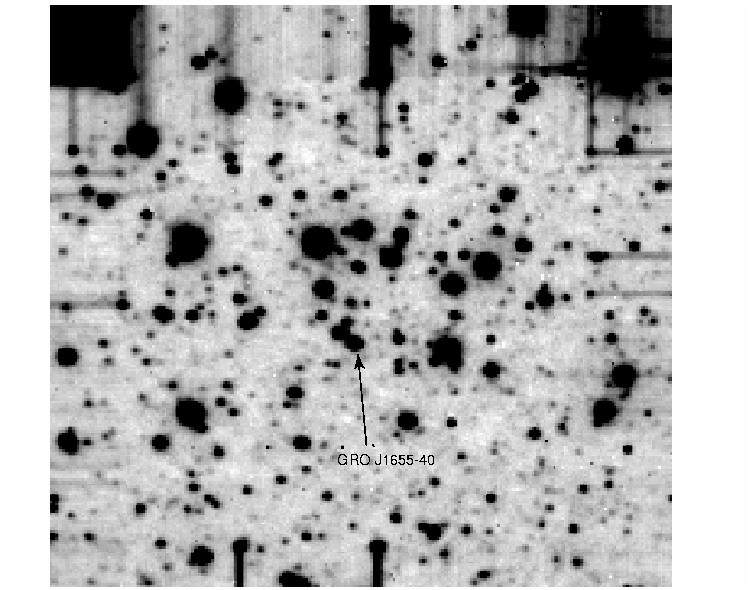
\includegraphics[width=5.0in]{ctio95_g001_3}
\caption{%
Example of an average combined grid of frames, with our system of interest
(\mbox{\groj}) indicated. This 15 second exposure, which has a
field of view of $\sim 166\arcsec \times 166\arcsec $, was
obtained using the CTIO CIRIM detector during June 1995.}\label{cha:lightcurve:sec:Photometry:subsec:CombiningTheGrid:fig:ctio95_g001_3}
\end{center}
\end{figure}
%%%%%%%%%%%%%%%%%%%%%%%%%%%%%%%%%%%%%%%%%%%%%%%%%%%%%%%%%%%%%%%%%%

Finally, each grid of images were combined to produce processed images of our target system (see \S~\vref{cha:InfraredDataReductionTechniques:sec:Photometry:subsec:CombiningTheGrid} for details). Figure~%
\vref{cha:lightcurve:sec:Photometry:subsec:CombiningTheGrid:fig:ctio95_g001_3}%
\ is an example of a combined grid from the 1995 $K_s$--band data set. %


%%%%%%%%%%%%%%%%%%%%%%%%%%%%% Relative Photometry %%%%%%%%%%%%%%%%%%%%

\subsection{Calculating the Relative Magnitudes}\label{cha:lightcurve:sec:Photometry:subsec:RelativePhotometry}

%%%%%%%%%%%%%%%%%%%%% 1648_1656_3 %%%%%%%%%%%%%%%%%%%%
\begin{figure}[!htb]
\begin{center}
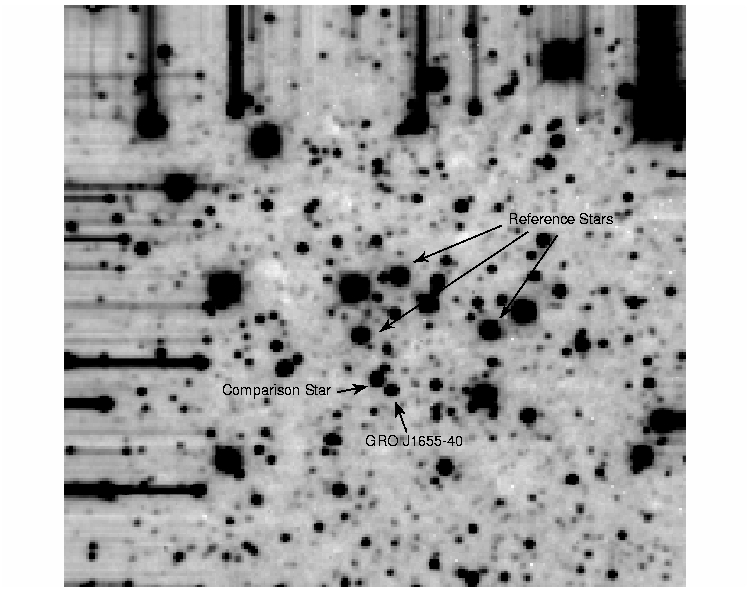
\includegraphics[width=5.0in]{1648_1656_3}
\caption{%
Field of view for the 1998 $K_s$ data, indicating the target,
comparison and reference stars. This $\sim 166\arcsec \times
166\arcsec$ image was obtained with a 30 second exposure using the
CTIO CIRIM detector during June 1998. }\label{cha:lightcurve:sec:Photometry:subsec:RelativePhotometry:fig:1648_1656_3}
\end{center}
\end{figure}
%%%%%%%%%%%%%%%%%%%%%%%%%%%%%%%%%%%%%%%%%%%%%%%%%%%%%%%%%%%%%%%%%%

Once the raw images were processed, we proceeded to run \texttt{DAOPHOT} to measure the magnitudes of \groj\ and a comparison star relative to several reference stars in the same field of view. The procedure outlined in \S~\ref{cha:InfraredDataReductionTechniques:sec:Photometry:subsec:RelativePhotometry} was  used for each period of observation and each filter. The stars chosen are given in Figure~%
\vref{cha:lightcurve:sec:Photometry:subsec:RelativePhotometry:fig:1648_1656_3}%
. %

%%%%%%%%%%%%%%%%%%%%%%%%%%%%% kctio98prefolded %%%%%%%%%%%%%%%%%%%%
\begin{figure}[!htb]
\begin{center}
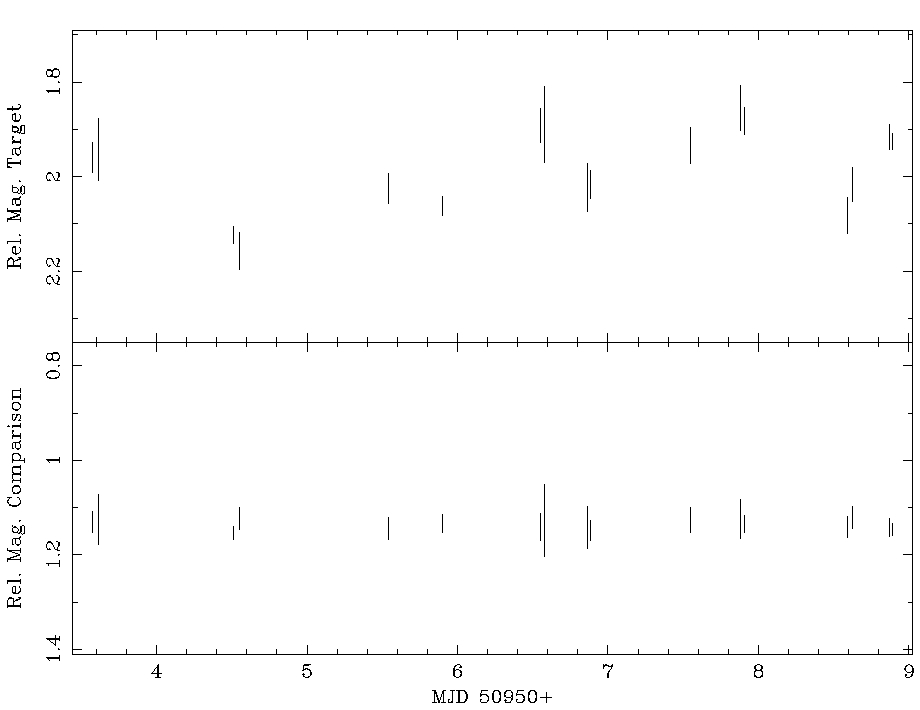
\includegraphics[width=5.0in]{kctio98prefolded}
\caption{%
Plot of relative magnitudes of target star \groj\ and comparison star
for the 1998 $K_s$ observations. %
}\label{cha:lightcurve:sec:Photometry:subsec:RelativePhotometry:fig:kctio98prefolded}
\end{center}
\end{figure}
%%%%%%%%%%%%%%%%%%%%%%%%%%%%%%%%%%%%%%%%%%%%%%%%%%%%%%%%%%%%%%%%%%

\vspace{\myparskip}

We then plotted the two relative magnitudes against the Julian
Dates of the observations to obtain the light curves of the target and
comparison star (see Figure~%
\ref{cha:lightcurve:sec:Photometry:subsec:RelativePhotometry:fig:kctio98prefolded}%
). Since the relative magnitude of the comparison star was constant over this period of observation, we assumed that the variability in the relative magnitude of \groj\ was due to the changing magnitude of the system itself. %

\vspace{\myparskip}

Finally, using the orbital
ephemeris determined by Van~der~Hooft et~al.\ %
\citeyear{VanDerHooft_et_al.:1998}%
\ (see \S~%
\vref{cha:GROJ1655-40:sec:IntroductionToJ1655:subsec:PropertiesOfJ1655:subsubsec:SystemProperties:eqn:Ephemeris}%
),%
\ we folded\footnote{\label{cha:lightcurve:sec:Photometry:subsec:RelativePhotometry:foot:MJD}%
When folding the data, the Heliocentric Julian Date (HJD) of the
observation was taken to be equal to the Julian Date (JD) of
observation. Although this introduced an error of 8 minutes, this is
small compared to the error in the orbital period ($2\fd62168\pm0\fd00014$:
van~der~Hooft et~al.\ %
\citeyearNP{VanDerHooft_et_al.:1998}%
).}%
\ the light curve of \groj\ on the orbital period. We then introduced
an offset to the 1998 $K_s$ data to move one of the points to phase
0.5, and so align the minima and maxima with the appropriate
phases. This offset was within the error of 3\% incurred by
extrapolating the ephemeris to the time of observation. %

%%%%%%%%%%%%%%%%%%%%%%%%%%%%% kctio95plot %%%%%%%%%%%%%%%%%%%%
\begin{figure}[!htb]
\begin{center}
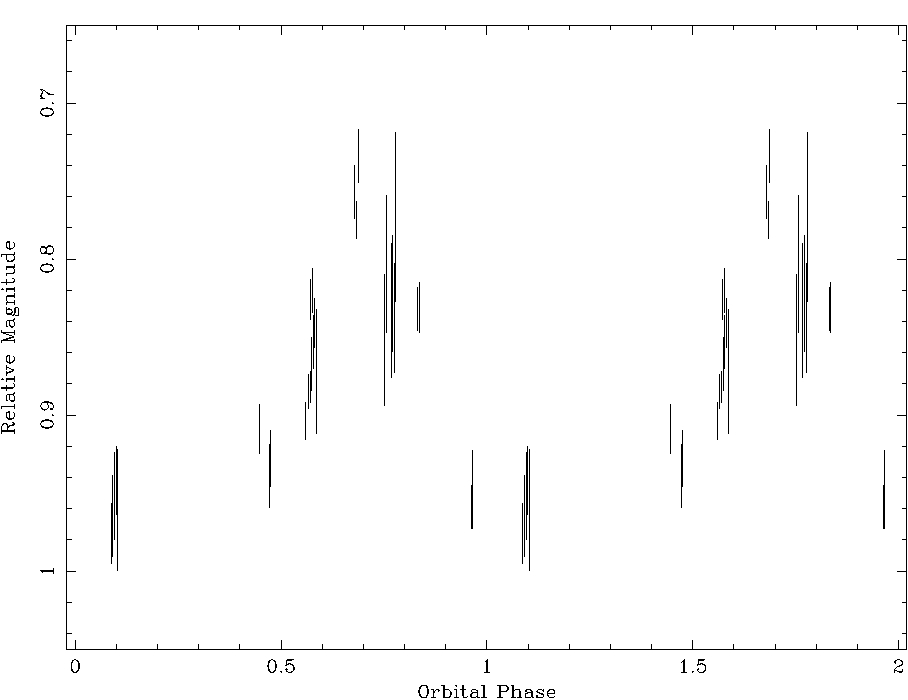
\includegraphics[width=5.0in]{kctio95plot}
\caption{%
The light curve of \groj\ during June 1995.
The fold is repeated for clarity. %
}\label{cha:lightcurve:sec:Photometry:subsec:RelativePhotometry:fig:kctio95plot}
\end{center}
\end{figure}
%%%%%%%%%%%%%%%%%%%%%%%%%%%%%%%%%%%%%%%%%%%%%%%%%%%%%%%%%%%%%%%%%%

\vspace{\myparskip}

Figure~%
\ref{cha:lightcurve:sec:Photometry:subsec:RelativePhotometry:fig:kctio95plot}%
\ and Figure~%
\ref{cha:lightcurve:sec:Photometry:subsec:RelativePhotometry:fig:kctio98plot}%
\ show the folded $K_s$ light curves for each year. As can be seen from Figure~%
\ref{cha:lightcurve:sec:Photometry:subsec:RelativePhotometry:fig:kctio98plot},%
\ an ellipsoidal variability was apparent from the 1998 $K_s$ light curve. %

%%%%%%%%%%%%%%%%%%%%%%%%%%%%% kctio98plot %%%%%%%%%%%%%%%%%%%%
\begin{figure}[!htb]
\begin{center}
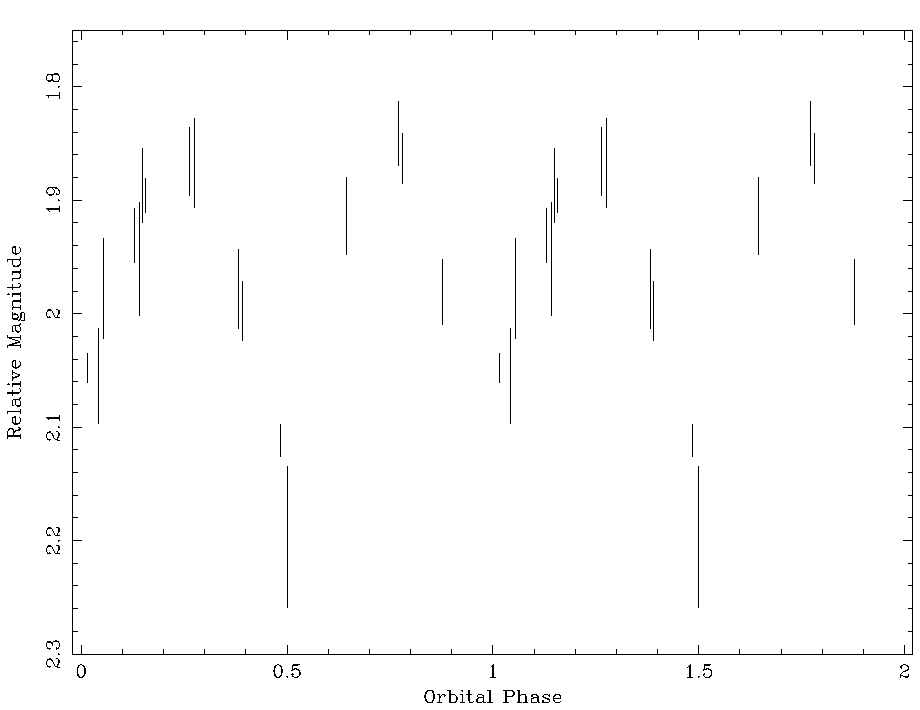
\includegraphics[width=5.0in]{kctio98plot}
\caption{%
The ellipsoidal variability of \groj\ during May-June 1998. %
}\label{cha:lightcurve:sec:Photometry:subsec:RelativePhotometry:fig:kctio98plot}
\end{center}
\end{figure}
%%%%%%%%%%%%%%%%%%%%%%%%%%%%%%%%%%%%%%%%%%%%%%%%%%%%%%%%%%%%%%%%%%

\vspace{\myparskip}

Using the folded light curves, we then calculated the phase averaged relative magnitudes of \groj\ (see \S~\ref{cha:InfraredDataReductionTechniques:sec:Photometry:subsec:RelativePhotometry:topic:parm}). Since the 1995 $J$--band data consisted of only one combined image, it was not
possible to get the phase average relative magnitude of \groj. The
relative magnitude of \groj\ in the single image was taken as the
average. Table~%
\vref{cha:lightcurve:sec:Photometry:subsec:RelativePhotometry:tab:phasemag}
lists the averaged magnitudes calculated.

\begin{table}[htb]
\caption{\groj\ Phase Averaged Relative Magnitudes}\label{cha:lightcurve:sec:Photometry:subsec:RelativePhotometry:tab:phasemag}

\begin{minipage}{\linewidth}
\renewcommand{\thefootnote}{\thempfootnote}

\begin{center}
\begin{tabular}{|l||||c|c|}

\hline
Year & $J$ Relative Magnitude (mag) & $K_s$ Relative Magnitude (mag) \\\hline\hline\hline\hline
1995 & $0.01\pm0.05$ & $0.68\pm0.05$ \\\hline
1998 & $1.00\pm0.05$ & $1.71\pm0.05$ \\\hline
\hline
\end{tabular}
\end{center}
\end{minipage}
\end{table}

%%%%%%%%%%%%%%%%%%%%%%%%%%%%% Apparent Magnitudes %%%%%%%%%%%%%%%%%%%%

\subsection{Obtaining the Apparent Magnitudes}\label{cha:lightcurve:sec:Photometry:subsec:PhotometricCalibration}

We next calculated the apparent magnitude of the system. We did this by photometrically calibrating our data. (See \S~\vref{cha:InfraredDataReductionTechniques:sec:Photometry:subsec:AperturePhotometry} for more details.) %

%%%%%%%%%%%%%%%%%%%%%%%%%%%%% CTIO CIRIM Images %%%%%%%%%%%%%%%%%%%%

\subsubsection{CTIO CIRIM Images}\label{cha:lightcurve:sec:Photometry:subsec:PhotometricCalibration:subsubsec:ctio}

We first attempted to calibrate the images using the observations made
with the CTIO CIRIM detector. Previously \citeN{Curran:2001} calculated the number of counts per second for a star of 10th magnitude ($f_{10}$) for the CTIO CIRIM detected. These values were:%
\begin{eqnarray} \label{cha:lightcurve:sec:Photometry:subsec:PhotometricCalibration:subsubsec:ctio:eqn:f10}
f_{10}(J) = 10,900\pm400\,\mathrm{counts/sec},\\\nonumber% chktex 35
f_{10}(K_s) = 6580\pm80\,\mathrm{counts/sec}.% chktex 35
\end{eqnarray} %

%%%%%%%%%%%%%%%%%%%%%%%%%%%%% 1648_1656_ctio_2 %%%%%%%%%%%%%%%%%%%%
\begin{figure}[!htb]
\begin{center}
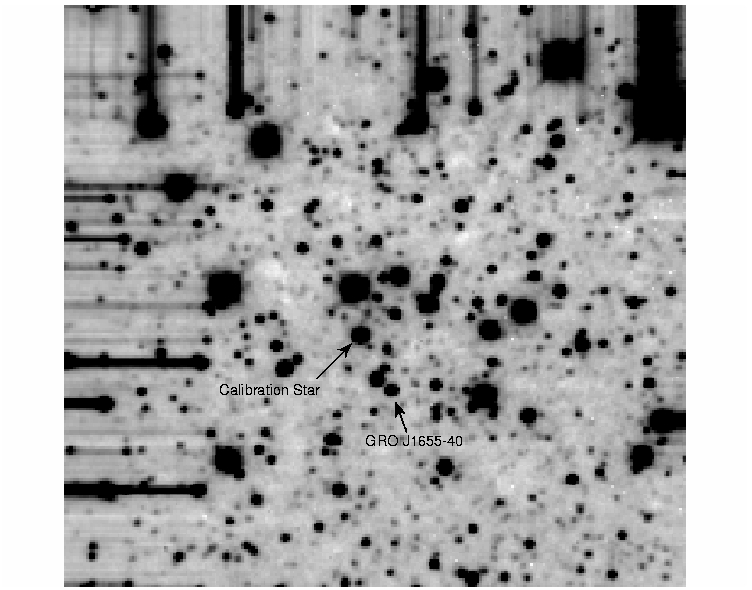
\includegraphics[width=5.0in]{1648_1656_ctio_2}
\caption{%
The selected photometric image from the 1998 $K_s$ data, with the
target star and calibration star indicated. This 30 second exposure,
with a field of view of $\sim 166\arcsec \times 166\arcsec $, was
obtained using the CTIO CIRIM detector during June 1998. }\label{cha:lightcurve:sec:Photometry:subsec:PhotometricCalibration:subsubsec:ctio:fig:1648_1656_ctio_2}
\end{center}
\end{figure}
%%%%%%%%%%%%%%%%%%%%%%%%%%%%%%%%%%%%%%%%%%%%%%%%%%%%%%%%%%%%%%%%%%

\vspace{\myparskip}

The log of the 1998 observations was consulted to determine
which of the original images were taken during photometric
conditions. One grid of such images was selected and aperture
photometry was performed on the combined image of this grid. The chosen image is shown in Figure~%
\vref{cha:lightcurve:sec:Photometry:subsec:PhotometricCalibration:subsubsec:ctio:fig:1648_1656_ctio_2}%
, and the calibration star is marked. %

\vspace{\myparskip}

\begin{table}[htb]
\caption{Apparent Magnitude of Calibration Star}\label{cha:lightcurve:sec:Photometry:subsec:PhotometricCalibration:subsubsec:ctio:tab:calibappmag}

\begin{minipage}{\linewidth}
\renewcommand{\thefootnote}{\thempfootnote}

\begin{center}
\begin{tabular}{|c|c|}

\hline
$J$ Apparent Magnitude (mag) & $K_s$ Apparent Magnitude (mag)\\\hline\hline\hline\hline
$12.81\pm0.05$ & $11.29\pm0.05$ \\\hline
\hline
\end{tabular}
\end{center}
\end{minipage}
\end{table}

The magnitudes of the comparison star in each filter are given in Table~%
\ref{cha:lightcurve:sec:Photometry:subsec:PhotometricCalibration:subsubsec:ctio:tab:calibappmag}%
.

\vspace{\myparskip}

\begin{table}[htb]
\caption{Initial \groj\ Apparent Magnitudes}\label{cha:lightcurve:sec:Photometry:subsec:PhotometricCalibration:subsubsec:ctio:tab:initappmag}

\begin{minipage}{\linewidth}
\renewcommand{\thefootnote}{\thempfootnote}

\begin{center}
\begin{tabular}{|l||||c|c|}

\hline
Year & $J$ Apparent Magnitude (mag) & $K_s$ Apparent Magnitude (mag)\\\hline\hline\hline\hline
1995 & $12.71\pm0.05$ & $11.98\pm0.05$ \\\hline
1998 & $13.81\pm0.05$ & $13.00\pm0.05$ \\\hline
\hline
\end{tabular}
\end{center}
\end{minipage}
\end{table}

Using these calibration magnitudes, the $K_s$--band and $J$--band magnitude of \groj\ were calculated as described in \S~\ref{cha:InfraredDataReductionTechniques:sec:Photometry:subsec:AperturePhotometry}. These values are listed in Table~%
\vref{cha:lightcurve:sec:Photometry:subsec:PhotometricCalibration:subsubsec:ctio:tab:initappmag}. The magnitudes calculated from the 1998 data were taken as the quiescent magnitudes of \groj, whereas the 1995 magnitudes were taken to be outburst magnitudes (see \S~\ref{cha:GROJ1655-40:sec:ObservationsOfJ1655:subsec:DetailsOfTheObservations}). It can be immediately seen that the system was brighter during outburst by approximately one magnitude. %


%%%%%%%%%%%%%%%%%%%%%%%%%%%%% KECK SCAM Images %%%%%%%%%%%%%%%%%%%%

\subsubsection{KECK SCAM Images}\label{cha:lightcurve:sec:Photometry:subsec:PhotometricCalibration:subsubsec:keck}

The second calibration was performed using the KECK observations of \\%
% WHITE SPACE %
\groj. Although these observations were not made under ideal photometric conditions, it was hoped that these images would provide a check for the earlier calibration. %

%%%%%%%%%%%%%%%%%%%%%%%%%%%%% keck00_2 %%%%%%%%%%%%%%%%%%%%
\begin{figure}[!htb]
\begin{center}
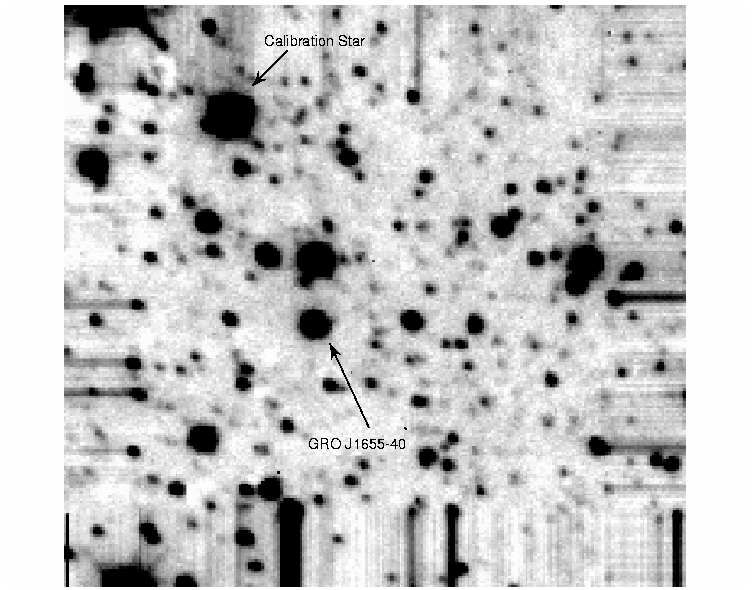
\includegraphics[width=5.0in]{keck00_2}
\caption{%
The field of view for the KECK images. The target star and the
calibration star are marked. This $\sim 46\arcsec \times 46\arcsec$
image was obtained with a $1\times10$ second exposure using the KECK
S-CAM detector during June 1998. }\label{cha:lightcurve:sec:Photometry:subsec:PhotometricCalibration:subsubsec:keck:fig:keck00_2}
\end{center}
\end{figure}
%%%%%%%%%%%%%%%%%%%%%%%%%%%%%%%%%%%%%%%%%%%%%%%%%%%%%%%%%%%%%%%%%%

\vspace{\myparskip}

During a KECK SCAM observation run prior to our run in 2000, the value of
$f_{10}$ was determined to be approximately 400,000 counts per second~\cite{Callanan:2001}%
. We applied aperture photometry to the calibration star in the
KECK images to measure the count rate $f$ of this star. Figure~%
\vref{cha:lightcurve:sec:Photometry:subsec:PhotometricCalibration:subsubsec:keck:fig:keck00_2}%
\ shows the processed KECK image with the calibration star
indicated. The apparent $K$--band magnitude, $K$, of the star was then
determined to be $11.25\pm0.05$\,mag. The apparent $K$ magnitude of \groj\ was then calculated, and found to be $12.95\pm0.05$\,mag. This value was consistent with the
preceding measurement using the 1998 CTIO images%
\footnote{\label{cha:lightcurve:sec:Photometry:subsec:PhotometricCalibration:foot:kks}
We take the magnitude of the star in the $K$-- and $K_s$--bands to be
equal.
}, validating the calibration. %

%%%%%%%%%%%%%%%%%%%%%%%%%%%%% 2MASS All-Sky Point Source Catalog %%%%%%%%%%%%%%%%%%%%

\subsubsection{2MASS All-Sky Point Source Catalog}\label{cha:lightcurve:sec:Photometry:subsec:PhotometricCalibration:subsubsec:2mass}

During the preparation of this thesis, the \textbf{All-Sky Point Source Catalog (PSC)} from the \textbf{Two Micron All Sky Survey (2MASS)}%
\footnote{\label{cha:lightcurve:sec:Photometry:subsec:PhotometricCalibration:subsubsec:2mass:foot:PSC}
\url{http://irsa.ipac.caltech.edu/}
}%
\ was released. We decided to verify our calibration of \groj\ using this more reliable source. %

\vspace{\myparskip}

\begin{table}[htb]
\caption{2MASS Apparent Magnitudes}\label{cha:lightcurve:sec:Photometry:subsec:PhotometricCalibration:subsubsec:2mass:tab:2massmags}

\begin{minipage}{\linewidth}
\renewcommand{\thefootnote}{\thempfootnote}

\DeclareFixedFootnote{\phase}{At Phase 0.21.} % For fixed footnote

\begin{center}
\begin{tabular}{|l||||c|c|}

\hline
Source & $J$ Apparent Magnitude (mag) & $K_s$ Apparent Magnitude (mag)\\\hline\hline\hline\hline
\groj\ \phase\ & $13.516\pm0.029$ & $12.744\pm0.034$ \\\hline
Calibration Star & $12.757\pm0.029$ & $11.153\pm0.021$ \\\hline
\hline
\end{tabular}
\end{center}
\end{minipage}
\end{table}

First, we obtained the apparent magnitudes of both our calibration star and \groj\ from the PSC --- see Table~%
\vref{cha:lightcurve:sec:Photometry:subsec:PhotometricCalibration:subsubsec:2mass:tab:2massmags}%
\ for these values. (We noted that the Modified Julian Date of the 2MASS observation of \groj\ was $51309.7443$, which corresponds to an orbital phase of approximately $0.21$.) %

\vspace{\myparskip}

\begin{table}[htb]
\caption{\groj\ Apparent Magnitudes}\label{cha:lightcurve:sec:Photometry:subsec:PhotometricCalibration:subsubsec:2mass:tab:appmag}

\begin{minipage}{\linewidth}
\renewcommand{\thefootnote}{\thempfootnote}

\begin{center}
\begin{tabular}{|l||||c|c|}

\hline
Year & $J$ Apparent Magnitude (mag) & $K_s$ Apparent Magnitude (mag)\\\hline\hline\hline\hline
1995 & $12.77\pm0.03$ & $11.83\pm0.04$ \\\hline
1998 & $13.76\pm0.03$ & $12.86\pm0.02$ \\\hline
\hline
\end{tabular}
\end{center}
\end{minipage}
\end{table}

\vspace{\myparskip}

As there was a slight discrepancy between our CTIO measurement of our calibration star and the values from 2MASS, we decided to assume the 2MASS magnitudes for the calibration star, due to the extra reliability of this source. We then used these values to calculate the apparent magnitude of \groj\ in both the $J$-- and $K_{s}$--bands. These magnitudes are listed in Table~%
\vref{cha:lightcurve:sec:Photometry:subsec:PhotometricCalibration:subsubsec:2mass:tab:appmag}. %

\begin{table}[htb]
\caption{Apparent Magnitude of \groj}\label{cha:lightcurve:sec:Photometry:subsec:PhotometricCalibration:tab:BeerGreeneMags}

\begin{minipage}{\linewidth}
\renewcommand{\thefootnote}{\thempfootnote}

\begin{center}
\begin{tabular}{|l||||c|c|}

\hline
Source & $J$ (mag) & $K$ (mag)\\\hline\hline\hline\hline
Our 1998 $K_{s}$--band Data & $13.76\pm0.03$ & $12.86\pm0.02$ \\\hline \citeN{GreeneBailynOrosz:2001} & $13.85\pm0.02$ & $13.25\pm0.02$ \\\hline
\citeN{BeerPodsiadlowski:2001} (predicted) & 13.8 & 13.0 \\\hline
\hline
\end{tabular}
\end{center}
\end{minipage}
\end{table}

\vspace{\myparskip}

Our values for the apparent magnitude of \groj\ during quiescence were
then compared to prior estimates, listed in Table~%
\vref{cha:lightcurve:sec:Photometry:subsec:PhotometricCalibration:tab:BeerGreeneMags}%
. Although our $J$--band value coincides with the two other values,
there is a 0.4 magnitude disagreement between our $K$--band value and
that of %
\citeN{GreeneBailynOrosz:2001}%
. A similar discrepancy has already been noted by %
\citeN{BeerPodsiadlowski:2001}%
, who obtained a theoretical magnitude in better agreement with our own. This suggests our result is valid, although why the discrepancy between \citeN{GreeneBailynOrosz:2001} and ourselves exists is unclear.

%%%%%%%%%%%%%%%%%%%%%%%%%%%%% Dereddened Magnitudes %%%%%%%%%%%%%%%%%%%%

\subsection{The Dereddened Magnitudes}\label{cha:lightcurve:sec:Photometry:subsec:DereddenedMagnitude}

We then corrected this magnitude to account for interstellar extinction. We obtained a value for the reddening, $E_{B-V}$, for \groj\ from Hynes et~al.\ %
\citeyear{Hynes_et_al.:1998}: %
\begin{eqnarray} \label{cha:lightcurve:sec:Photometry:subsec:DereddenedMagnitude:eqn:EBV}
E_{B-V} = 1.2\pm0.1 \ \mathrm{mag}.
\end{eqnarray}
We derived the $K$-- and $J$--band extinction following the discussion on page~%
\pageref{cha:InfraredDataReductionTechniques:sec:Photometry:subsec:DereddenedMagnitude:eqn:CardelliAK},%
\ and obtained the values of $A_{K} = 0.42\pm0.04$\,mag and $A_{J} = 1.05\pm0.09$\,mag. (Note that the values for interstellar extinction in the infrared is much lower than that in the optical, which is given by $A_{V} = 1.3\times3.1=4.0\pm0.3$\,mag. This is as expected --- see \S~\vref{cha:InfraredDataReductionTechniques:sec:InfraredAstronomy:subsubsec:InterstellarExtinction}.) The \textbf{dereddened magnitudes} %
of \groj\ in the $J$-- and $K$--band were then calculated, and are summarised in Table~%
\vref{cha:lightcurve:sec:Photometry:subsec:DereddenedMagnitude:tab:Dered}.
The difference of 1\,mag between both the two values for $K_0$ and those
for $J_0$ were attributed to the contribution from the disk during
the outburst in 1995. %

\begin{table}[htb]
\caption{Dereddened $J$, $K$ and $J-K$ Magnitudes for 1995 and 1998}\label{cha:lightcurve:sec:Photometry:subsec:DereddenedMagnitude:tab:Dered}

\begin{minipage}{\linewidth}
\renewcommand{\thefootnote}{\thempfootnote}

\begin{center}
\begin{tabular}{|l||||c|c|c|}

\hline
Year & $J_0$ (mag)& $K_0$ (mag)& $J_{0}-K_{0}$ (mag) \\\hline\hline\hline\hline
1995 & $11.72\pm0.09$ & $11.41\pm0.06$ & $0.3\pm0.1$ \\\hline
1998 & $12.71\pm0.09$ & $12.44\pm0.04$ & $0.3\pm0.1$ \\\hline
\hline
\end{tabular}
\end{center}
\end{minipage}
\end{table}

\vspace{\myparskip}

Using the derived values of $K_0$ and $J_0$, we calculated the
dereddened \mbox{$J-K$} colour of \groj\ for 1995 and 1998. These values are also given in Table~%
\ref{cha:lightcurve:sec:Photometry:subsec:DereddenedMagnitude:tab:Dered}%
.

\vspace{\myparskip}

\begin{table}[htb]
\caption{Comparison Dereddened Magnitudes}\label{cha:lightcurve:sec:Photometry:subsec:DereddenedMagnitude:tab:BeerGreeneDeredMag}

\begin{minipage}{\linewidth}
\renewcommand{\thefootnote}{\thempfootnote}

\DeclareFixedFootnote{\pred}{From their predicted apparent magnitudes.} % For fixed footnote

\begin{center}
\begin{tabular}{|l||||c|c|c|}

\hline
Source & $J_0$ (mag)& $K_0$ (mag)& $J_{0}-K_{0}$ (mag) \\\hline\hline\hline\hline
\citeN{GreeneBailynOrosz:2001} & $12.80\pm0.09$ & $12.83\pm0.04$ & $0.0\pm0.1$ \\\hline
\citeN{BeerPodsiadlowski:2001}\pred\ & 12.75 & 12.58 & 0.17 \\\hline
\hline
\end{tabular}
\end{center}
\end{minipage}
\end{table}

Finally, we calculated the dereddened magnitudes using the apparent magnitudes calculated by %
\citeN{GreeneBailynOrosz:2001}%
\ and those predicted by %
\citeN{BeerPodsiadlowski:2001}%
. Table~%
\ref{cha:lightcurve:sec:Photometry:subsec:DereddenedMagnitude:tab:BeerGreeneDeredMag}%
\ lists these values. Again, our value for $J_{0}-K_{0}$ during quiescence
is in good agreement with that predicted by %
\citeN{BeerPodsiadlowski:2001}%
, but differs from that of %
\citeN{GreeneBailynOrosz:2001}%
. It should however be noted that in general $J_{0}-K_{0}>0$, which
supports our earlier conclusion that the $K$ magnitude derived by %
\citeN{GreeneBailynOrosz:2001}%
\ may be erroneous. %

\vspace{\myparskip}

According to %
\citeN{BeerPodsiadlowski:2001}%
, the spectral type of \groj\ lies within the range F5--G0 III-IV.\@\ We
compared our dereddened $J-K$ with that of UKIRT standard stars with a
spectral type similar to \groj. We found that the value
$J_{0}-K_{0}=0.3$\,mag was consistent with a spectral type of F0--G2
III-IV, which is in agreement with, if not as precise as, the spectral range of \citeN{BeerPodsiadlowski:2001}. %


%%%%%%%%%%%%%%%%%%%%%%%%%%%%% Absolute Magnitude %%%%%%%%%%%%%%%%%%%%

\subsection{The Absolute Magnitudes}\label{cha:lightcurve:sec:Photometry:subsec:AbsoluteMagnitude}

As a final check for self-consistency in our derived value for the magnitude of \groj, we calculated the absolute $J$-- and $K$--magnitudes of this system using Equations~%
\ref{cha:InfraredDataReductionTechniques:sec:MagnitudeScale:subsec:AbsoluteMagnitude:eqn:AbsMagK}%
\ and~\ref{cha:InfraredDataReductionTechniques:sec:MagnitudeScale:subsec:AbsoluteMagnitude:eqn:AbsMagJ}%
. We assumed a distance of 3.2\,kpc for this calculation~\cite{HjellmingRupen:1995}%
. These magnitudes are tabulated in Table~%
\vref{cha:lightcurve:sec:Photometry:subsec:AbsoluteMagnitude:tab:absmag}. %

\begin{table}[htb]
\caption{$J$ and $K$ Absolute Magnitudes of \groj\ }\label{cha:lightcurve:sec:Photometry:subsec:AbsoluteMagnitude:tab:absmag}

\begin{minipage}{\linewidth}
\renewcommand{\thefootnote}{\thempfootnote}

\begin{center}
\begin{tabular}{|l||||c|c|}

\hline
Year & $M_J$ (mag) & $M_K$ (mag) \\\hline\hline\hline\hline
1995 & $-0.8\pm0.2$ & $-1.1\pm0.2$ \\\hline
1998 & $0.2\pm0.2$ & $-0.1\pm0.2$ \\\hline
\hline
\end{tabular}
\end{center}
\end{minipage}
\end{table}

\vspace{\myparskip}

We then compared the absolute magnitudes from 1998 with the quiescent
absolute magnitudes of several other SXTs, namely \mbox{GRS 1121--68}, \mbox{A0620--00} and \mbox{V404
Cyg}, some of the properties of which are given in Table~%
\vref{cha:lightcurve:sec:Photometry:subsec:AbsoluteMagnitude:tab:pdSXTs}%
. We consulted the literature for the relevant $J$ and $K$ magnitudes
and the interstellar reddening of these systems, and calculated the
absolute magnitude of each. Table~%
\vref{cha:lightcurve:sec:Photometry:subsec:AbsoluteMagnitude:tab:absmagSXTs}%
\ lists the derived absolute magnitudes. %

\begin{table}[htb]
\caption{Periods and Distances of Comparison SXTs}\label{cha:lightcurve:sec:Photometry:subsec:AbsoluteMagnitude:tab:pdSXTs}%

\begin{minipage}{\linewidth}
\renewcommand{\thefootnote}{\thempfootnote}

\DeclareFixedFootnote{\cc91}{Callanan \& Charles (1991).} % For fixed footnote
\DeclareFixedFootnote{\pc}{Callanan et~al.\ (1996).} % For fixed footnote
\DeclareFixedFootnote{\snc}{Shahbaz, Naylor, \& Charles (1993).} % For fixed footnote
\DeclareFixedFootnote{\chaty}{Chaty et~al.\ (2002).} % For fixed footnote
\DeclareFixedFootnote{\fron}{Froning \& Robinson (2001).} % For fixed footnote
\DeclareFixedFootnote{\srbncc}{Shahbaz et~al.\ (1994).} % For fixed footnote
\DeclareFixedFootnote{\ccn}{Casares, Charles, \& Naylor (1992).} % For fixed footnote
\DeclareFixedFootnote{\elvis}{Elvis et~al.\ (1975).} % For fixed footnote
\DeclareFixedFootnote{\shah4}{Shahbaz et~al.\ (1997).} % For fixed footnote
\DeclareFixedFootnote{\bailyn}{Bailyn (1992).} % For fixed footnote

\begin{center}
\begin{tabular}{|l||||c|c|}

\hline

        & P           & $d$ (kpc) \\\hline\hline\hline\hline

%GS 2000+25 & $8\fh2$\cc91 & 2\pc   \\\hline
%Cen X-4    & $15\fh12$\snc & 1.2\snc \\\hline
GRS 1121--68 & $10\fh5$\bailyn\ & 2.8\shah4\ \\\hline
A0620--00  & $7\fh75$\fron\ & 1\elvis\   \\\hline
V404 Cyg   & $6\fd5$\ccn\ & 3.5\srbncc\    \\\hline

\hline
\end{tabular}
\end{center}
\end{minipage}
\end{table}

\nocite{Callanan_et_al.:1996b}%
\nocite{CallananCharles:1991}%
\nocite{ShahbazNaylorCharles:1993}%
\nocite{Chaty_et_al.:2002}%
\nocite{FroningRobinson:2001}%
\nocite{Shahbaz_et_al.:1994}%
\nocite{CasaresCharlesNaylor:1992}
\nocite{Elvis_et_al.:1975}
\nocite{Bailyn:1992}
\nocite{Shahbaz_et_al.:1997}

\begin{table}[htb]
\caption{Absolute Magnitudes of SXTs}\label{cha:lightcurve:sec:Photometry:subsec:AbsoluteMagnitude:tab:absmagSXTs}%

\begin{minipage}{\linewidth}
\renewcommand{\thefootnote}{\thempfootnote}

\DeclareFixedFootnote{\pc}{Callanan et~al.\ (1996).} % For fixed footnote
\DeclareFixedFootnote{\snc}{Shahbaz, Naylor, \& Charles (1993).} % For fixed footnote
\DeclareFixedFootnote{\chaty}{Chaty et~al.\ (2002).} % For fixed footnote
\DeclareFixedFootnote{\fron}{Froning \& Robinson (2001).} % For fixed footnote
\DeclareFixedFootnote{\srbncc}{Shahbaz et~al.\ (1994).} % For fixed footnote
\DeclareFixedFootnote{\blair}{Calculated assuming $E_{B-V} = 0.1$\,mag
(Blair et~al.\ 1984).} % For fixed footnote
\DeclareFixedFootnote{\pcd}{Derived from the $A_V$ value of 4.1 mag
from Callanan et~al.\ (1996).} % For fixed footnote
\DeclareFixedFootnote{\srbnccd}{Computed using $A_V=2.8$ (Shahbaz
et~al.\ 1994).} % For fixed footnote
\DeclareFixedFootnote{\van}{Calculated using $E_{B-V}=0.35$\,mag
(van~Paradijs \& McClintock 1995).} % For fixed footnote

\begin{center}
\begin{tabular}{|l||||c|c|c|}

\hline
        & $J$ (mag) & $A_J$ (mag) & $M_J$ (mag) \\\hline\hline\hline\hline

GRS 1121--68 & 17.5\chaty\  & 0.35\chaty\ & 4.99\chaty\ \\\hline
A0620--00  & 15.6\fron\ & 0.31\van\ & 5.29  \\\hline\hline\hline\hline

        & $K$ (mag) & $A_K$ (mag) & $M_K$ (mag) \\\hline\hline\hline\hline

GRS 1121--68 & 16.7\chaty\ & 0.14\chaty\ & 4.33\chaty\ \\\hline
A0620--00  & 14.5\fron\ & 0.12\van\ & 4.38 \\\hline
V404 Cyg   & 12.4\srbncc\ & 0.32\srbnccd\ & -0.64 \\\hline


\hline
\end{tabular}
\end{center}
\end{minipage}
\end{table}

\nocite{Callanan_et_al.:1996b}%
\nocite{ShahbazNaylorCharles:1993}%
\nocite{Chaty_et_al.:2002}%
\nocite{FroningRobinson:2001}%
\nocite{Shahbaz_et_al.:1994}%
\nocite{Blair_et_al.:1984}
\nocite{VanParadijsMcClintock:1995}

\vspace{\myparskip}

The absolute magnitude of \groj\ is more consistent with that of
\mbox{V404 Cyg}, a result which is to be expected as both systems are
long period binaries, whereas the other SXTs are short period systems.

%%%%%%%%%%%%%%%%%%%%%%%%%%%%% Modelling the Light Curve of GRO J1655-40 %%%%%%%%%%%%%%%%%%%%

\section{Modelling the Light Curve of \groj}\label{cha:lightcurve:sec:ModellingTheLightCurve}

In this chapter, we have demonstrated how we obtained a measure of the ellipsoidal variability of \groj\ during quiescence.
In the next chapter, we will explain how we employed numerical simulations of this light curve to obtain a value for
the mass ratio $q$ and the binary inclination $i$ of our target system. %

%%%%%%%%%%%%%%%%%%%%%%%%%%%%% End of Chapter %%%%%%%%%%%%%%%%%%%%

% chktex-file 44
%%%%%%%%%%%%%%%%%%%%%%%%%%%% ELC %%%%%%%%%%%%%%%%%%%%

\chapter{The Eclipsing Light Curve Code}\label{cha:ELC}

Having obtained the light curve of \groj, we attempted to model the data through numerical simulations of the X-ray binary. Here we outline the components of the model, and discuss the values obtained for the mass ratio and inclination.

%%%%%%%%%%%%%%%%%%%%%%%%%%%%% Introduction to ELC %%%%%%%%%%%%%%%%%%%%

\section{Introduction to \textit{ELC}}\label{cha:ELC:sec:IntroductionELC}

The \textbf{Eclipsing Light Curve} (\textit{ELC}) code%
\footnote{\label{cha:ELC:sec:IntroductionELC:foot:ELC}
We ran version 2 of this program, as described by the author in %
\citeN{OroszHauschildt:2000:cantcheck}%
}%
\ was written by Jerome A.\ Orosz, of the Universiteit Utrecht in
the Netherlands\footnote{\label{cha:ELC:sec:IntroductionELC:foot:Orosz}%
The author is now in San Diego State University. %
}%
. This suite of programs creates a theoretical model of a star
system, based on a user-specified set of parameters, such as the mass
ratio and orbital inclination of a binary system. It then modifies the
light curve until it obtains the best fit to the observations of the
user. %

\vspace{\myparskip}

The \textit{ELC} programs can model the light curve of:
\begin{itemize}


\item
\textbf{a binary star system}: for example, an X-ray binary, where the
companion star is denoted by star 1 and the compact star by star 2. %

\item
\textbf{a binary system with an accretion disk}, such as an X-ray binary with
a disk around the compact object (star 2). %

\end{itemize}
The component stars can have eccentric orbits, and the effect of
mutual eclipses of the accretion disk and secondary star can be
included in the model. %

\vspace{\myparskip}

The three \textit{ELC} programs that were employed in our modelling were:

\begin{itemize}

\item \texttt{ELC}%
\footnote{\label{cha:ELC:sec:IntroductionELC:foot:ELCabbrev}
Note that the abbreviation ELC can refer to either the suite of
programs (referred to in this text by the use of italics:
\textit{ELC}) or this specific program (referred to by using typewriter
font: \texttt{ELC}). }%
, which creates light curve models (in linear units) for several passbands
based on a list of system parameters. %

\item \mbox{\texttt{gridELC}}, an optimizer based on the ``grid search''
routine~\cite{Bevington:1969}. Given a series of folded light curves and radial velocity curves,
\mbox{\texttt{gridELC}} will adjust user-specified parameters to find the
minimum $\Chi^2$ of the fit of the \textit{ELC} model to the data. The
final set of parameters are then used to create light curve models
(in linear units).

\item \mbox{\texttt{checkfit}}, which converts the linear
\texttt{gridELC} model to magnitudes and then scales it according to the
data. %

\end{itemize}

We utilised these \textit{ELC} programs to model both the 1998 and
1995 data sets. %

%%%%%%%%%%%%%%%%%%%%%%%%%%%%% 1998 $K_s$--band Data %%%%%%%%%%%%%%%%%%%%

\section{The 1998 $K_s$--band Data}\label{cha:ELC:sec:1998Results}

%%%%%%%%%%%%%%%%%%%%%%%%%%%%% Details of Model %%%%%%%%%%%%%%%%%%%%

\subsection{Details of the Quiescent Model}\label{cha:ELC:sec:1998Results:subsec:model}

The quiescent observations of \groj\ were modelled by accounting only
for the ellipsoidal variability of the secondary star. The disk contribution to
the overall flux of the system was assumed to be negligible (we will later show this to
be a valid assumption --- see \S~%
\vref{cha:AccretionDiskContamination:sec:Spectroscopy:subsec:DiskContribution}%
), and hence we assumed there would be no noticeable eclipse of the
accretion disk. It was also assumed that there was no X-ray heating of
the secondary star. The model we employed was of a binary system
with a Roche lobe filling secondary star and a black hole primary
star. %

%%%%%%%%%%%%%%%%%%%%%%%%%%%%% Modelling Procedure %%%%%%%%%%%%%%%%%%%%

\subsection{Modelling Procedure for the 1998 Data}\label{cha:ELC:sec:1998Results:subsec:ModellingProcedure}

The following procedure details how we modelled the 1998 observations
of \\%
% WHITE SPACE %
\groj\ using the described model. %

\begin{itemize}

\item
We obtained a folded light curve for the 1998 $K_s$--band observations
(see \S~%
\vref{cha:lightcurve:sec:Photometry:subsec:RelativePhotometry}%
). This light curve was phased according to the convention of %
\citeN{OroszBailyn:1997}%
\ which places star 1 (with filled Roche lobe) in front of the compact star 2 at phase 0.0. See
Figure~%
\vref{cha:lightcurve:sec:Photometry:subsec:RelativePhotometry:fig:kctio98plot}%
\ for the plot of this light curve. %

\begin{table}[htb]
\caption{Fixed \textit{ELC} Binary System Parameters}\label{cha:ELC:sec:1998Results:subsec:ModellingProcedure:tab:FixELCBinaryParms}

\begin{minipage}{\linewidth}
\renewcommand{\thefootnote}{\thempfootnote}


\DeclareFixedFootnote{\beerstellar}{Corresponding to a star of spectral type
F5--G0 III-IV (Beer \& Podsiadlowski 2001).} % For fixed footnote
\DeclareFixedFootnote{\pringle}{This close binary should have synchronously rotating components in a circular orbit.} % For fixed footnote %(Pringle 1985)
\DeclareFixedFootnote{\ob97}{Orosz \& Bailyn (1997).} % For fixed footnote
\DeclareFixedFootnote{\vdh98}{van~der~Hooft et~al.\ (1998).} % For fixed footnote
\DeclareFixedFootnote{\shah}{Shahbaz et~al.\ (1999).} % For fixed footnote
\DeclareFixedFootnote{\beer}{Beer \& Podsiadlowski (2001) --- these values were only initially fixed.} % For fixed footnote
\DeclareFixedFootnote{\bh}{\textit{ELC} interprets this to mean that the primary star is an invisible black hole.} % For fixed footnote

\begin{center}
\begin{tabular}{|l||||l|c|}

\hline
Name        & Description                & Value \\\hline\hline\hline\hline
Q        & Mass ratio                 & 3.9\beer\ \\\hline
finc        & Inclination                 & $68\fdg65$\beer\ \\\hline
Tgrav1      & Gravity Darkening exponent, star 1    & 0.25\vdh98\ \\\hline
Period        & Orbital period of binary            & 2 \fd\ 62168\vdh98 \\\hline
betarim        & Angle of disk to orbital plane     & $\sim 2\degr$\ob97  \\\hline
alb1        & Bolometric albedo, star 1        & 0.5\ob97\\\hline
fm        & Mass function, star 2            & 2.73\,M\ensuremath{_{\odot}}\shah\ \\\hline
separ        & Orbital separation            & $\sim16$\,R\ensuremath{_{\odot}}\shah\ \\\hline
Teff1        & Mean temperature, star 1        & $\sim6400$\,K\beerstellar\ \\\hline
Teff2        & Mean temperature, star 2        & $<0$\,K\bh\ \\\hline
fill1        & Roche lobe filling factor, star 1     & 1.000%
\footnote{\label{cha:ELC:sec:1998Results:subsec:ModellingProcedure:tab:FixELCBinaryParms:foot:mass}%
Since accretion continues in quiescence (see \S~\vref{cha:Introduction:sec:X--rayBinaries:subsec:Quiescence}). }%
\\\hline
fill2        & Roche lobe filling factor, star 2    & 0.000%
\footnote{\label{cha:ELC:sec:1998Results:subsec:ModellingProcedure:tab:FixELCBinaryParms:foot:bh}
Primary star is a black hole.}%
\\\hline
eccen        & Eccentricity of orbit            & 0\pringle\ \\\hline
omega1        & Ratio of rotational to orbital frequency, star 1 & 1\pringle\ \\\hline
omega2        & Ratio of rotational to orbital frequency, star 2 & 1\pringle\ \\\hline

\hline

\end{tabular}
\end{center}
\end{minipage}
\end{table}

\nocite{OroszBailyn:1997}
\nocite{Shahbaz_et_al.:1999}
%\nocite{Pringle:1985}
\nocite{BeerPodsiadlowski:2001}

\begin{table}[htb]
\caption{Fixed \textit{ELC} Parameters}\label{cha:ELC:sec:1998Results:subsec:ModellingProcedure:tab:FixELCParms}

\begin{minipage}{\linewidth}
\renewcommand{\thefootnote}{\thempfootnote}

\begin{center}
\begin{tabular}{|l||||l|c|}

\hline
Name        & Description                & Value \\\hline\hline\hline\hline
Nalph1, Nalph2     & Number of latitude grid elements     & 100 \\\hline
Nbet1, Nbet2    & Number of longitude grid elements     & 35  \\\hline
Ntheta        & Number of azimuthal grid points    & 90 \\\hline
Nradius        & Number of radial grid points        & 80 \\\hline
ilaw        & Controls form of limb darkening law    & 1 (Linear
law)  \\\hline

\hline

\end{tabular}
\end{center}
\end{minipage}
\end{table}

\item
The literature was consulted for values of the parameters in Table~%
\vref{cha:ELC:sec:1998Results:subsec:ModellingProcedure:tab:FixELCBinaryParms}%
. The values for the parameters in Table~%
\vref{cha:ELC:sec:1998Results:subsec:ModellingProcedure:tab:FixELCParms} %
were set from experience. %

\begin{table}[htb]
\caption{Values of Variable \textit{ELC} Parameters for 1998 Data}\label{cha:ELC:sec:1998Results:subsec:ModellingProcedure:tab:VarELCParms}

\begin{minipage}{\linewidth}
\renewcommand{\thefootnote}{\thempfootnote}
\DeclareFixedFootnote{\nodisk}{No disk present.} % For fixed footnote
\DeclareFixedFootnote{\nolx}{No X-ray heating.} % For fixed footnote
\DeclareFixedFootnote{\noeclipse}{No eclipses.} % For fixed footnote

\begin{center}
\begin{tabular}{|l||||l|c|}

\hline
Name        & Description &    Value \\\hline\hline\hline\hline
iecheck & Switch for eclipses & -1\noeclipse\  \\\hline
idint & Switch for disk       & 0\nodisk\ \\\hline
rinner        & Inner radius of disk  & --\nodisk\ \\\hline
router        & Outer radius of disk    & --\nodisk\ \\\hline
xi        & Power-law exponent on the disk temperature profile &
--\nodisk\ \\\hline
tdisk        & Temperature of inner disk & --\nodisk\ \\\hline
Nref        & Number of iterations for reflection effect & 0\nolx\ \\\hline
Lx        & $\log_{10}{L_{X}}$ for primary star in X-ray binary
& 0\nolx\ \\\hline

\hline

\end{tabular}
\end{center}
\end{minipage}
\end{table}

\item
Since this model ignored X-ray heating and the accretion disk, the
parameters in Table~%
\vref{cha:ELC:sec:1998Results:subsec:ModellingProcedure:tab:VarELCParms} %
were set to the appropriate values. %

\item
\texttt{ELC} was run without a input file to produce a
\textbf{parameter file} with each parameter
set to its default value. This file was edited, setting the parameters
to the values shown in Tables~%
\ref{cha:ELC:sec:1998Results:subsec:ModellingProcedure:tab:FixELCBinaryParms}%
--%
\ref{cha:ELC:sec:1998Results:subsec:ModellingProcedure:tab:VarELCParms}. %
The remaining parameters were left at their default values.

\item
\texttt{ELC} was run once more, this time using the \textbf{edited}
input file. This created a model binary system based on the values
given for the system parameters, and outputted this in both
linear and magnitude units to a data file. %

\item
The parameter file for \mbox{\texttt{gridELC}} was edited, to specify
both the folded light curve data file and the parameters to be adjusted, namely the
mass ratio and inclination. %

\item
\mbox{\texttt{gridELC}} was run. The final values calculated for the adjusted
parameters were noted.

\item
The $\Chi^2$ value of the fit of the model to the observations was
determined using \mbox{\texttt{checkfit}}, from which the reduced
chi-squared%
\footnote{\label{cha:ELC:sec:IntroductionELC:foot:chi2}
%(\citeN{McCarthy:1999} p.~19) %
The reduced chi-squared ($\Chi^{2}_{\nu}$) of the fit is defined by: %
\[ \Chi^{2}_{\nu} = \frac{\Chi^2}{n-p-1}, \]
where $n$ is the number of the data points and $p$ is the number of
parameters of the fit. A $\Chi^{2}_{\nu}$ value of approximately 1 was
desired. }%
\ was calculated. %

\item The resultant model plot and the light curve data were
superimposed for a visual check of the fit. %
\end{itemize}%

%%%%%%%%%%%%%%%%%%%%%%%%%%%%% Comparison of Model and Results %%%%%%%%%%%%%%%%%%%%

\subsection{Comparison of Quiescent Model and Results}\label{cha:ELC:sec:1998Results:subsec:comparison}%

%%%%%%%%%%%%%%%%%%%%%%%%%%%%% kctio98fit %%%%%%%%%%%%%%%%%%%%
\begin{figure}[!htb]%
\begin{center}%
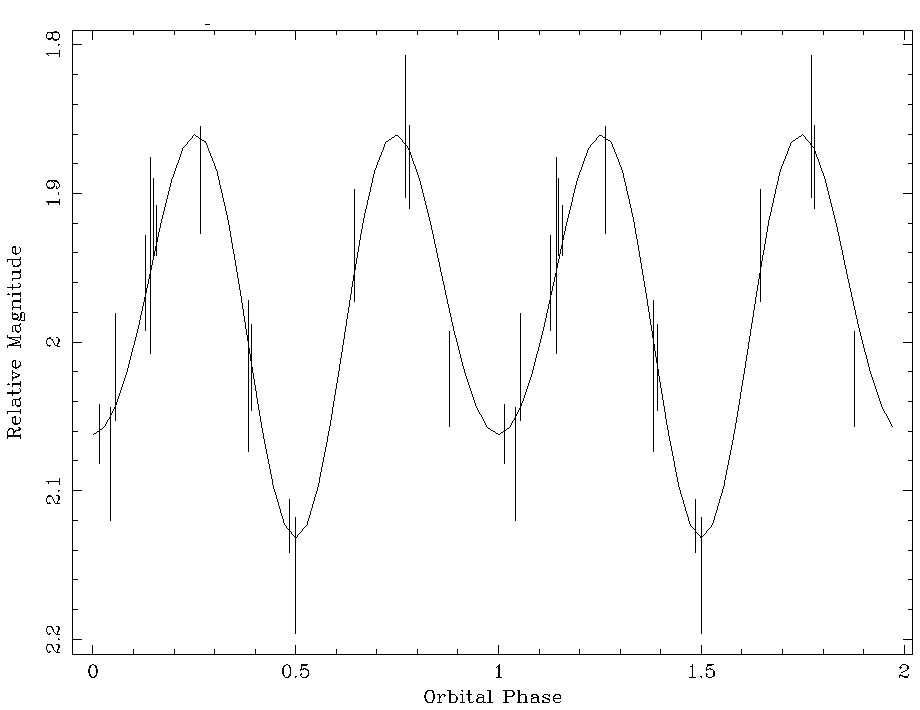
\includegraphics[width=5.0in]{kctio98fit}%
\caption{%
The observed $K_s$ light curve for \groj\ in May/June 1998, together with a theoretical light curve computed for a mass ratio of $2$ and a binary inclination of $69\degr$. %
Two orbital cycles are shown for clarity.}\label{cha:ELC:sec:1998Results:subsec:comparison:fig:kctio98fit}%
\end{center}%
\end{figure}%
%%%%%%%%%%%%%%%%%%%%%%%%%%%%%%%%%%%%%%%%%%%%%%%%%%%%%%%%%%%%%%%%%%

As can be seen in Figure~%
\vref{cha:ELC:sec:1998Results:subsec:comparison:fig:kctio98fit}%
, the data were well modelled by our theoretical light curve, and we
obtained $\Chi_{\nu}^{2} = 0.51$ as the reduced chi-squared%
\footnote{\label{cha:ELC:sec:1998Results:foot:LowError}
We interpret this low $\Chi_{\nu}^{2}$ value as signifying that
\texttt{DAOPHOT} is overestimating the errors for the estimates of the
relative magnitude of \groj. }. %
The theoretical light curve mimics the ellipsoidal variability of the
secondary, with the expected deeper minimum at phase 0.5. %

%%%%%%%%%%%%%%%%%%%%%%%%%%%%% Derived Mass Ratio and Inclination %%%%%%%%%%%%%%%%%%%%

\subsubsection{Derived Mass Ratio and Inclination}\label{cha:ELC:sec:1998Results:subsec:comparison:subsubsec:derivedQ}

%%%%%%%%%%%%%%%%%%%%%%%%%%%%% contourPlot2  %%%%%%%%%%%%%%%%%%%%
\begin{figure}[!htb]
\begin{center}
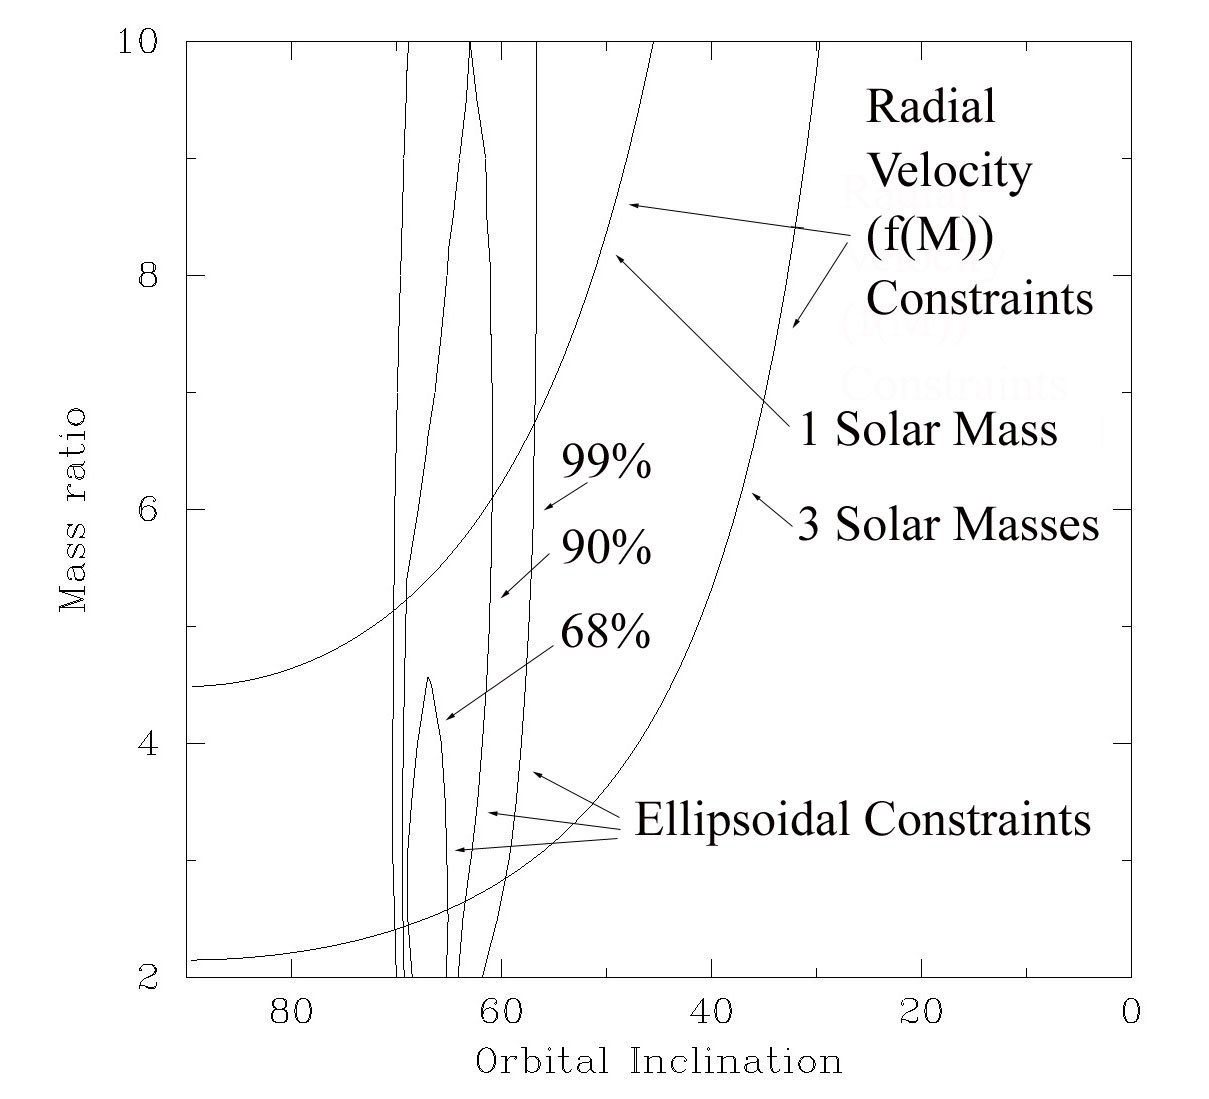
\includegraphics[width=5.0in]{contourPlot2}
\caption{%
The $\chi^2$ contour plot for the 1998 $K_{s}$--band data. This plot displays the 68\%, 90\% and
 99\% confidence levels from the \texttt{ELC} fits, together with constraint curves derived from the mass function assuming a secondary mass of 1\,M\sun\ and 3\,M\sun, respectively. (The minimum reduced $\chi^2$ has been set equal to 1.) %
}\label{cha:ELC:sec:1995Results:subsec:comparison:fig:contourPlot2}
\end{center}
\end{figure}

%%%%%%%%%%%%%%%%%%%%%%%%%%%%%%%%%%%%%%%%%%%%%%%%%%%%%%%%%%%%%%%%%%

In order to properly constrain the mass ratio and the inclination, \texttt{gridELC} was run to create a $\Chi^{2}$ contour plot. We simultaneously varied the inclination between $i=0\degr$ and $i=90\degr$ and the mass ratio between $q=2$ and $q=10$, and computed the $\Chi^{2}$ of the fit using \texttt{gridELC}. Figure~%
\vref{cha:ELC:sec:1995Results:subsec:comparison:fig:contourPlot2}%
\ shows the resultant plot, together with constraints for $i$ and $q$
derived from the mass function and secondary mass considerations,
assuming (conservatively) that the mass of the secondary lies between 1\,M\sun\ and
3\,M\sun\ --- it is an F/G (sub)giant.% chktex 36
The area in Figure~\ref{cha:ELC:sec:1995Results:subsec:comparison:fig:contourPlot2}
where the mass function and ellipsoidal modelling constraints overlap denotes the allowed values of $q$ and $i$.
Generally, our results show that the inclination of the system lies in the range $i=64\degr$--$70\degr$,
and that the mass ratio lies in the range $q=2.5$--$6$, at the 90\% confidence level. %

\vspace{\myparskip}

Table~%
\vref{cha:ELC:sec:1998Results:tab:ComparisonOfResults}%
\ compares the values we derived for the mass ratio $q$ and the
inclination $i$ of \groj\ with those from other studies of this system. From this table, it can be seen that the values for both our mass ratio and orbital inclination are
consistent with past estimates. %

\begin{table}[htb]
\caption{Comparison of Derived Values for $q$ and $i$}\label{cha:ELC:sec:1998Results:tab:ComparisonOfResults}

\begin{minipage}{\linewidth}
\renewcommand{\thefootnote}{\thempfootnote}

\begin{center}
\begin{tabular}{|l||||c|c|}

\hline
Data Set            & $q$          & $i$ \\\hline\hline\hline\hline
Our 1998 $K_s$--band Data     & $2.5-6$     & $64\degr-70\degr$
\\\hline
\citeN{BeerPodsiadlowski:2001} (Predicted) & $3.9\pm0.6$    & $68\fdg65\pm1\fdg5$ \\\hline
\citeN{GreeneBailynOrosz:2001}    & $2.6\pm0.3$    & $70\fdg2\pm1\fdg9$ \\\hline
\citeN{Shahbaz_et_al.:1999}    & 2.29--2.97 & --- \\\hline
van~der~Hooft et~al.\ \citeyear{VanDerHooft_et_al.:1998}    & 2.43--4.20     & $63\fdg7$--$70\fdg7$\\\hline
\citeN{OroszBailyn:1997}    & $2.99\pm0.08$    & $69\fdg50\pm0\fdg08$ \\\hline

\hline

\end{tabular}
\end{center}
\end{minipage}
\end{table}


%%%%%%%%%%%%%%%%%%%%%%%%%%%%% Derived Component Masses %%%%%%%%%%%%%%%%%%%%

\subsubsection{Derived Component Masses}\label{cha:ELC:sec:1998Results:subsec:comparison:subsubsec:derivedm}

Using our values for $q$ from the 1998 data ($q=2.5$--$6$) and the
corresponding secondary masses ($M_{2}=1$--$3$\,M\sun), we derived the
mass of the primary as $6.8\pm0.7$\,M\sun. This is to be compared in particular with the results from the only other infrared study of this system, which yielded $M_{X}=6.3\pm0.5$\,M\sun\~\cite{GreeneBailynOrosz:2001}. Table~%
\vref{cha:ELC:sec:1998Results:subsec:comparison:subsubsec:derivedm:tab:ComparisonOfResults}%
\ compares this mass with masses from earlier studies. %

\begin{table}[htb]
\caption{Comparison of Derived Values for $M_X$}\label{cha:ELC:sec:1998Results:subsec:comparison:subsubsec:derivedm:tab:ComparisonOfResults}

\begin{minipage}{\linewidth}
\renewcommand{\thefootnote}{\thempfootnote}

\begin{center}
\begin{tabular}{|l||||c|c|}

\hline
Data Set            & $M_X$ (M\sun)      \\\hline\hline\hline\hline
Our 1998 $K_s$--band Data     & $6.8\pm0.7$        \\\hline % 2002Bin2SimpleMassInc
\citeN{BeerPodsiadlowski:2001} (Predicted) & $5.4\pm0.3$    \\\hline
\citeN{GreeneBailynOrosz:2001}    & $6.3\pm0.5$    \\\hline
\citeN{Shahbaz_et_al.:1999}    & 5.5--7.9 \\\hline
van~der~Hooft et~al. \citeyear{VanDerHooft_et_al.:1998}    & 6.29--7.20     \\\hline
\citeN{OroszBailyn:1997}    & $7.02\pm0.22$    \\\hline

\hline

\end{tabular}
\end{center}
\end{minipage}
\end{table}

\vspace{\myparskip}

Our values are consistent with preceding results, and is above the
standard limit for neutron star masses. This implies that the compact
object in \groj\ is a black hole, if we accept the neutron star mass limit of \citeN{RhoadesRuffini:1974}. We note however that this result is dependent on the assumption of negligible disk contamination. %

%%%%%%%%%%%%%%%%%%%%%%%%%%%%% 1995 $K_s$--band Data %%%%%%%%%%%%%%%%%%%%

\section{The 1995 $K_s$--band Data}\label{cha:ELC:sec:1995Results}

%%%%%%%%%%%%%%%%%%%%%%%%%%%%% Details of Model %%%%%%%%%%%%%%%%%%%%

\subsection{Details of Outburst Model}\label{cha:ELC:sec:1995Results:subsec:model}

The model for the outburst of \groj\ included:
\begin{inparaenum}[(i)]
\item
the ellipsoidal variability of the Roche lobe filling secondary,
\item
a bright hot accretion disk and
\item
eclipses of the accretion disk and the secondary.
\end{inparaenum}

%%%%%%%%%%%%%%%%%%%%%%%%%%%%% Modelling Procedure %%%%%%%%%%%%%%%%%%%%

\subsection{Modelling Procedure for the 1995 Data}\label{cha:ELC:sec:1995Results:subsec:ModellingProcedure}

\begin{table}[htb]
\caption{Values of Variable \textit{ELC} Parameters for 1995 Data Set}\label{cha:ELC:sec:1995Results:subsec:ModellingProcedure:tab:paramvalues}

\begin{minipage}{\linewidth}
\renewcommand{\thefootnote}{\thempfootnote}

\DeclareFixedFootnote{\steady}{Assuming a steady-state disk.} % For fixed footnote
\DeclareFixedFootnote{\diskp}{Accretion disk present.} % For fixed footnote
\DeclareFixedFootnote{\eclipse}{Check for eclipses.} % For fixed footnote
\DeclareFixedFootnote{\nolx}{No X-ray heating.} % For fixed footnote

\begin{center}
\begin{tabular}{|l||||l|}

\hline
Name        & Value \\\hline\hline\hline\hline
iecheck     & 0\eclipse\ \\\hline
idint         & 1\diskp\ \\\hline
rinner        & 0.55   \\\hline
router        & 1.0      \\\hline
xi        & $-0.8$\steady\ \\\hline
tdisk        & $\sim 13000$\,K \\\hline
Nref        & 0\nolx\ \\\hline
Lx        & 0\nolx\ \\\hline

\hline

\end{tabular}
\end{center}
\end{minipage}
\end{table}

The procedure for modelling the 1995 $K_s$ observations was
essentially the same as for the 1998 data. Here, we outline the main
differences:

\begin{itemize}

\item
The variable parameters were set as to include an accretion disk and
eclipses --- see Table~%
\vref{cha:ELC:sec:1995Results:subsec:ModellingProcedure:tab:paramvalues}%
. %

\item
Rather than attempting to vary the mass ratio and inclination, we
fixed these parameters to the values obtained from the quiescent data,
and applied these values in our attempt to fit the outburst data.

\end{itemize}

%%%%%%%%%%%%%%%%%%%%%%%%%%%%% Comparison of Model and Results %%%%%%%%%%%%%%%%%%%%

\subsection{A Poor Fit}\label{cha:ELC:sec:1995Results:subsec:comparison}

%%%%%%%%%%%%%%%%%%%%%%%%%%%%% kctio95fixedfit %%%%%%%%%%%%%%%%%%%%
\begin{figure}[!htb]
\begin{center}
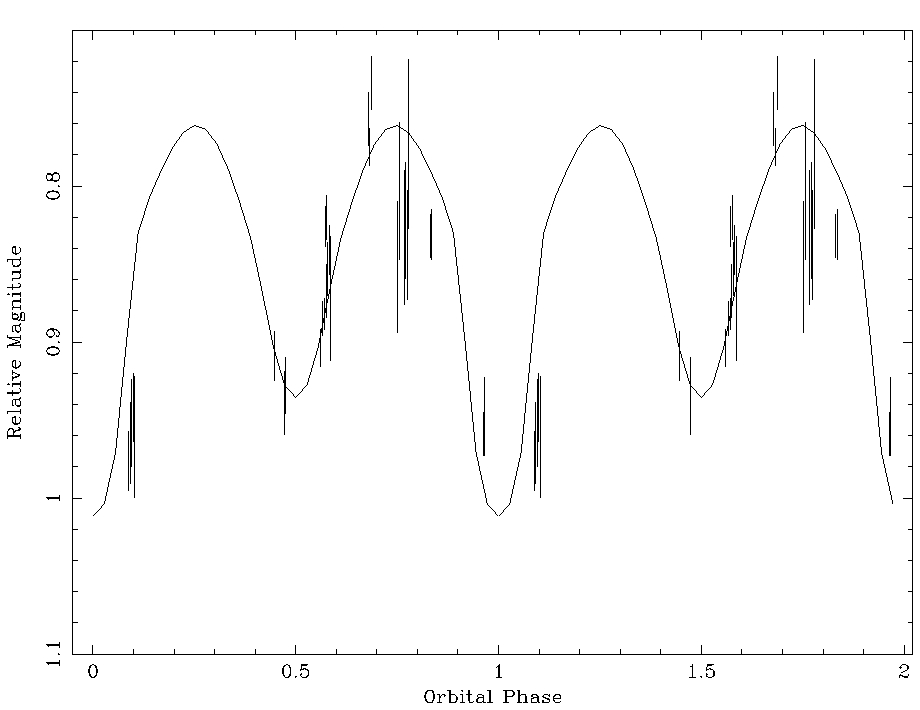
\includegraphics[width=5.0in]{kctio95fixedfit}
\caption{%
The June 1995 $K_s$ light curve of \groj, with a model
light curve using the mass ratio and inclination from the best fits of
the 1998 data set ($q=2$, $i=69\degr$). %
}\label{cha:ELC:sec:1995Results:subsec:comparison:fig:kctio95fixedfit}
\end{center}
\end{figure}
%%%%%%%%%%%%%%%%%%%%%%%%%%%%%%%%%%%%%%%%%%%%%%%%%%%%%%%%%%%%%%%%%%

Figure~%
\vref{cha:ELC:sec:1995Results:subsec:comparison:fig:kctio95fixedfit}%
\ shows the resultant fit of our model to the outburst data. We
obtained a reduced chi-squared of $\Chi_{\nu}^{2} = 5.89$. The fit is much poorer than for the 1998 data, for the reasons we now outline. %

%%%%%%%%%%%%%%%%%%%%%%%%%%%%% The Accretion Disk %%%%%%%%%%%%%%%%%%%%

\subsubsection{The Accretion Disk}\label{cha:ELC:sec:1995Results:subsec:comparison:subsubsec:disk}

Since \groj\ was in outburst at the time of these observations, the
flux from the accretion disk was more significant than the ellipsoidal
variability of the secondary star. The deeper minimum at phase 0 is
indicative of an eclipse of the bright accretion disk by the
secondary star. The presence of eclipses agrees well with the high
orbital inclination of this system. %

\vspace{\myparskip}

We note that there is no evidence of an eclipse of the accretion disk
in the quiescent light curve, even though \groj\ has been shown to be
an eclipsing binary from the outburst observations, and in spite of the high inclination ($i\sim70\degr$) of the system. This is consistent
with the negligible disk contribution to the overall flux from the
system during quiescence. %

\vspace{\myparskip}

The reduced $\Chi^2$ values obtained for the outburst data are
significantly higher than the quiescent values. One possible
explanation for this is that the accretion disk is significantly
non-axisymmetric, or exhibits infrared flaring or flickering activity, which the code is unable to account for. %
\citeN{OroszBailyn:1997}%
\ were also unable to accurately model their optical outburst data, taken
during August 1994 and March-April 1995, and obtained larger reduced
$\Chi^2$ values from modelling their outburst data than from their quiescent data. %

%%%%%%%%%%%%%%%%%%%%%%%%%%%%% Amplitude of Variability %%%%%%%%%%%%%%%%%%%%

%%%%%%%%%%%%%%%%%%%%%%%%%%%% Confirming Our Assumption of Negligible Disk Contribution
 %%%%%%%%%%%%%%%%%%%%

\section{Does the Accretion Disk Contribute?}\label{cha:ELC:sec:ConfirmingOurAssumption}

Although we have now obtained a plausible value for the mass of the black hole in \groj, we made the assumption that the contribution of the accretion disk in the infrared was negligible. In the following chapter, we explain how we confirmed this assumption from infrared spectroscopy of the binary system.

%%%%%%%%%%%%%%%%%%%%%%%%%%%%% End of Chapter %%%%%%%%%%%%%%%%%%%%

%%%%%%%%%%%%%%%%%%%%%%%%%%%%% Accretion Disk Contamination %%%%%%%%%%%%%%%%%%%%

\chapter{The Accretion Disk Contamination}
\label{cha:AccretionDiskContamination}

Although we have now obtained a value for the mass of the black hole in \\%
% WHITE SPACE %
\groj, this is not  be a reliable estimate, unless we first confirm that the disk contamination is negligible in this system. Here we discuss the application of infrared spectroscopic techniques to determine from the spectral features of \groj the contribution of the accretion disk. %

%%%%%%%%%%%%%%%%%%%%%%%%%%%%% Spectroscopy of \groj %%%%%%%%%%%%%%%%%%%%

\section{Spectroscopy of \groj}
\label{cha:AccretionDiskContamination:sec:Spectroscopy}

We processed the NIRSPEC data as follows to obtain spectra from which we could accurately measure the absorption and emission features present in the spectrum of \groj.

%%%%%%%%%%%%%%%%%%%%%%%%%%%%% Initial Reduction %%%%%%%%%%%%%%%%%%%%

\subsection{The Initial Reduction}
\label{cha:AccretionDiskContamination:sec:Spectroscopy:subsec:InitialReduction}

We first subtracted the background from the spectra of our target \groj, and also for the spectra
of \mbox{HD 326320}, an A0 star (see page~%
\pageref{cha:GROJ1655-40:sec:ObservationsOfJ1655:subsec:DetailsOfTheObservations:subsubsec:2000Spectroscopy}%
), as outlined in \S~\ref{cha:InfraredDataReductionTechniques:sec:SpectroscopyData:subsec:BackgroundSubtraction}. %

\vspace{\myparskip}

The gain and read noise for the NIRSPEC detector were
obtained from the instrument webpage%
\footnote{%
\label{cha:AccretionDiskContamination:sec:Spectroscopy:subsec:InitialReduction:foot:Nirspec}
\url{http://www2.keck.hawaii.edu:3636/realpublic/inst/nirspec/nirspec.html} }%
. 1-D spectra were then extracted from the background subtracted images, using
these parameter values in \textit{apall}. (See \S~\ref{cha:InfraredDataReductionTechniques:sec:SpectroscopyData:subsec:SpectraExtraction} for details.) %

\vspace{\myparskip}

A dispersion correction was calculated and applied to the spectra using the \texttt{identify} and \texttt{reidentify} tasks: %
\begin{inparaenum}[(i)]
\item
We obtained an Argon arc lamp map from the webpage%
\footnote{%
\label{cha:AccretionDiskContamination:sec:Spectroscopy:subsec:InitialReduction:foot:CGS4}
\url{http://www.jach.hawaii.edu/JACpublic/UKIRT/instruments/cgs4/} }%
\ of the UKIRT CGS4 detector, containing accurate wavelengths of
numerous spectral lines.
\item
These lines were marked on one of the
extracted Ar arc spectra.
\item
The corresponding vacuum wavelengths were
entered into the \texttt{identify} database.
\item
A cubic spline function
was fitted to these data.
\item
Significantly bad data points
were identified and removed, and a new fit was applied, with a rms of
1.6\,\AA.
\item The function was then applied to identify the spectral lines in the other
extracted arc spectra, using the task \texttt{reidentify}. %
\end{inparaenum}

\vspace{\myparskip}

Each of the spectra of \groj\ and \mbox{HD 326320}
was then assigned one of the arc spectra using
\texttt{refspectra}. The cubic fits calculated from \texttt{identify}
and \texttt{reidentify} were used by \texttt{dispcor} to dispersion
correct the extracted target spectra. %

\vspace{\myparskip}

The wavelength-calibrated spectra were then normalised by using the
task \texttt{continuum} to fit the continuum of each spectrum to a
spline of order 2. %

%%%%%%%%%%%%%%%%%%%%%%%%%%%%% Removing the Telluric Features %%%%%%%%%%%%%%%%%%%%

\subsection{Removing the Telluric Features}
\label{cha:AccretionDiskContamination:sec:Spectroscopy:subsec:TelluricFeatures}

Having obtained normalised spectra of our system, we next removed the features in the spectra that were due to atmospheric absorption (see \S~\ref{cha:InfraredDataReductionTechniques:sec:SpectroscopyData:subsec:TelluricFeatures}). We had chosen the A0-type star \mbox{HD 326320} to act as our comparison star, due to the scarcity of prominent features in the $K$--band. We masked the only major feature (Br-$\gamma$) in the comparison star spectra, and the target star spectra were then divided by the
resultant spectrum. %

%%%%%%%%%%%%%%%%%%%%%%%%%%%%% The Final Spectrum %%%%%%%%%%%%%%%%%%%%

\subsection{Our Spectrum of \groj}
\label{cha:AccretionDiskContamination:sec:Spectroscopy:subsec:CombiningTheSpectra}

%%%%%%%%%%%%%%%%%%%%%%%%%%%%% j1655editedMasked %%%%%%%%%%%%%%%%%%%%
\begin{figure}[!htb]
\begin{center}
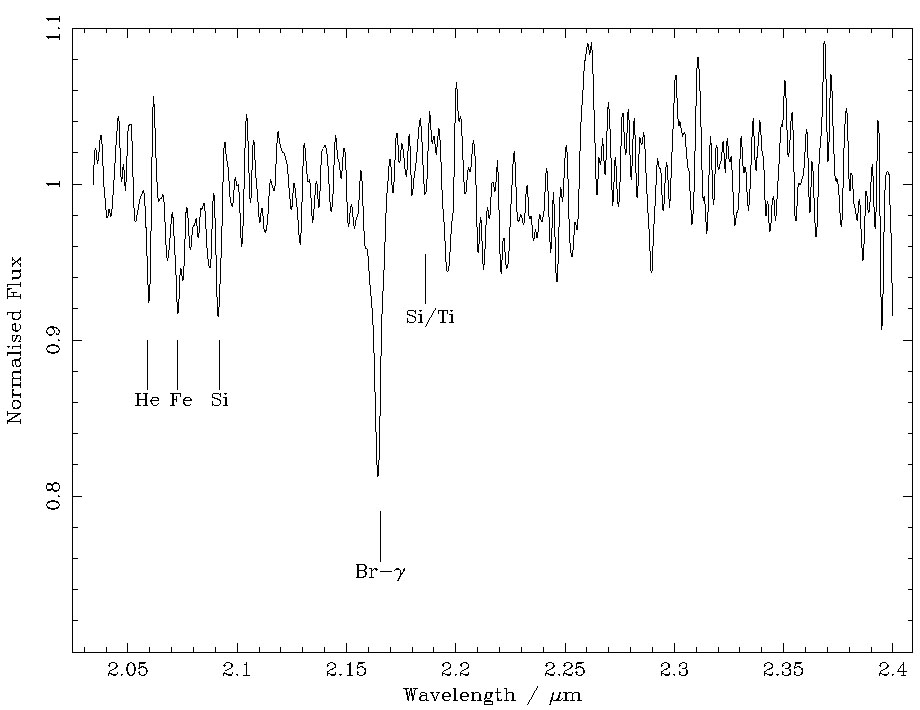
\includegraphics[width=5.0in]{j1655editedMasked}
\caption{%
The $K$--band spectrum of \groj, having been corrected for telluric
features with reference to an A0 star. The dominant Br-$\gamma$
feature is marked, together with several weaker features. }
\label{cha:AccretionDiskContamination:sec:Spectroscopy:subsec:CombiningTheSpectra:fig:j1655editedMasked}
\end{center}
\end{figure}
%%%%%%%%%%%%%%%%%%%%%%%%%%%%%%%%%%%%%%%%%%%%%%%%%%%%%%%%%%%%%%%%%%

The final spectrum was obtained by combining the two corrected target spectra, and smoothing the resultant spectrum, as we explained in \S~\ref{cha:InfraredDataReductionTechniques:sec:SpectroscopyData:subsec:CombiningTheSpectra}. Our spectrum of \groj\ is shown in Figure~%
\ref{cha:AccretionDiskContamination:sec:Spectroscopy:subsec:CombiningTheSpectra:fig:j1655editedMasked}%
. %

%%%%%%%%%%%%%%%%%%%%%%%%%%%%% Disk Contribution %%%%%%%%%%%%%%%%%%%%

\subsection{Determining the Disk Contribution}
\label{cha:AccretionDiskContamination:sec:Spectroscopy:subsec:DiskContribution}

%%%%%%%%%%%%%%%%%%%%%%%%%%%%% combinedSpectra %%%%%%%%%%%%%%%%%%%%
\begin{figure}[!htb]
\begin{center}
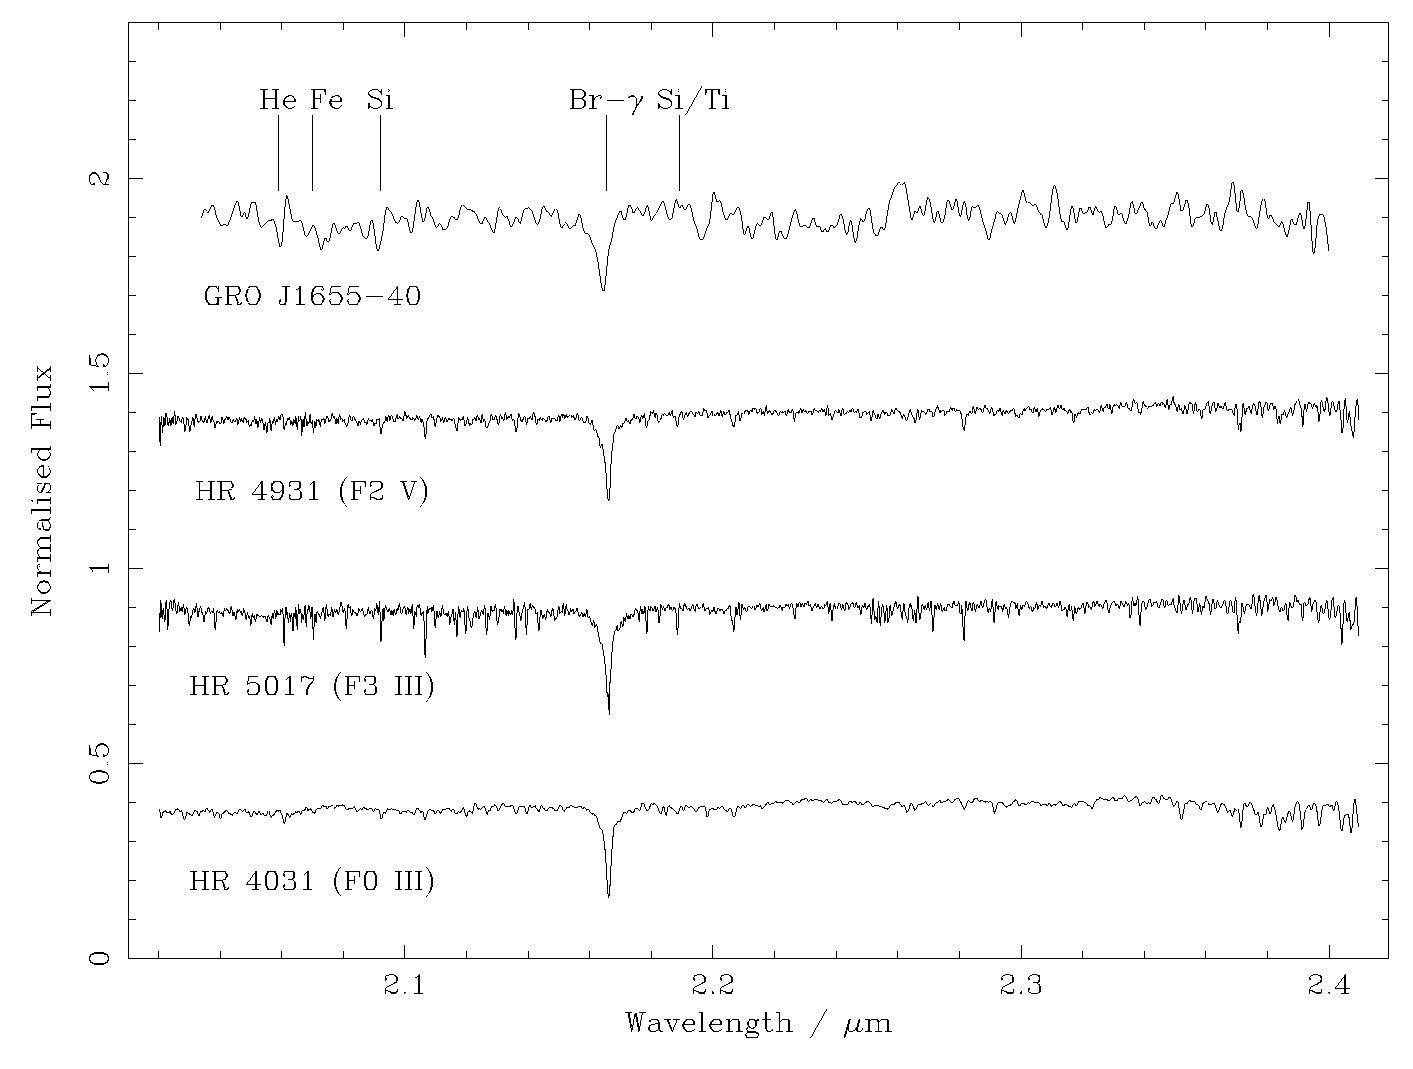
\includegraphics[width=5.0in]{combinedSpectra}
\caption{%
The $K$--band spectra of GRO J1655--40, HR 4031, HR 5017 and HR 4931, with the
spectral features of interest marked.}
\label{cha:AccretionDiskContamination:sec:Spectroscopy:subsec:DiskContribution:fig:combinedSpectra}
\end{center}
\end{figure}
%%%%%%%%%%%%%%%%%%%%%%%%%%%%%%%%%%%%%%%%%%%%%%%%%%%%%%%%%%%%%%%%%%


In order to determine the degree of accretion disk contamination in
\groj, we compared our spectrum of this system with spectra of
isolated stars of similar spectral type to the secondary in \groj. We
obtained these comparison spectra from the literature, and calculated
the equivalent width (see
\S~%
\vref{cha:InfraredDataReductionTechniques:sec:Spectroscopy:subsec:EquivalentWidth}%
) of the Br-$\gamma$ absorption feature in the target and comparison
spectra. If the Br-$\gamma$ feature in our spectrum of \groj\ was
significantly weaker than the corresponding features in the sample
spectra, this would imply that there was emission present in the $K$--band from the
disk. %

\vspace{\myparskip}

\begin{table}[htb]
\caption{Equivalent widths of Br-$\gamma$ feature}
\label{cha:AccretionDiskContamination:sec:Spectroscopy:subsec:AbsenceOfDiskContribution:tab:WallaceWidths}

\begin{minipage}{\linewidth}
\renewcommand{\thefootnote}{\thempfootnote}

\begin{center}
\begin{tabular}{|l|l|c||||l|l|c|}

\hline
Identifier & Spectral Type & $W_{\lambda}/$\AA & Identifier & Spectral
Type & $W_{\lambda}/$\AA \\\hline\hline\hline\hline
\groj\  & F5--G0 III--IV & $10\pm1$ & \mbox{HR 4931} & F2 V & $8\pm1$ \\\hline
\mbox{HR 7495} & F5 II--III & $7.0\pm0.5$ & \mbox{HR 6927} & F7 V & $4.0\pm0.5$ \\\hline
\mbox{HR 4031} & F0 III     & $8.5\pm0.5$ & \mbox{HR 6608} & G2 IIIb & $3.0\pm0.5$ \\\hline
\mbox{HR 5017} & F3 III     & $8\pm1$     & \mbox{HR 7373} & G8 IV & $3\pm1$ \\\hline
\mbox{HR 21}   & F2 IV      & $7\pm1$     & \mbox{HR 4375} & G0 V & $3\pm1$ \\\hline
\mbox{HR 8905} & F8 IV      & $4.5\pm0.5$ & \mbox{HR 483}  & G1.5 V & $3.5\pm0.5$ \\\hline
\mbox{HR 2943} & F5 IV-V    & $6.5\pm0.5$ & \mbox{HR 7504} & G3 V & $3.0\pm0.5$ \\\hline
\hline
\end{tabular}
\end{center}
\end{minipage}
\end{table}

The isolated stars with spectral types of F5--G0 III--IV (the spectral
type of \groj: see %
\citeNP{BeerPodsiadlowski:2001}%
) were chosen from the spectral atlas
of %
\citeN{WallaceHinkle:1997}%
. Figure~%
\vref{cha:AccretionDiskContamination:sec:Spectroscopy:subsec:DiskContribution:fig:combinedSpectra}%
\ displays three of the chosen spectra%
\footnote{%
\label{cha:AccretionDiskContamination:sec:Spectroscopy:subsec:DiskContribution:foot:wavenumber}%
The spectra were originally plotted with flux as a function of inverse wavenumber, but we converted them to $\mu$m for comparison with our spectrum. %
}%
, together with our spectrum of \groj. The equivalent widths of the Br-$\gamma$ absorption features in the telluric-corrected spectrum of \groj\ and the above stars were measured using \texttt{splot}. Table~%
\vref{cha:AccretionDiskContamination:sec:Spectroscopy:subsec:AbsenceOfDiskContribution:tab:WallaceWidths}%
\ lists these equivalent widths. %

\vspace{\myparskip}

As can be clearly seen, the equivalent width for \groj\ agrees well
with certain stars, namely \mbox{HR 4031}, \mbox{HR 5017} and \mbox{HR
4931}. This implies that the disk contributes little light to the
system in the $K$--band, and also that the spectral type of the secondary
star in \groj\ is within the range F5--F7 III--IV, which is consistent
with our initial range of F0--G2 III--IV, derived in \S~%
\vref{cha:lightcurve:sec:Photometry:subsec:DereddenedMagnitude}%
. %

\vspace{\myparskip}

\begin{table}[htb]
\caption{Equivalent widths of weaker features}
\label{cha:InfraredDataReductionTechniques:sec:Spectroscopy:subsec:AbsenceOfDiskContribution:tab:Weaker}

\begin{minipage}{\linewidth}
\renewcommand{\thefootnote}{\thempfootnote}

\begin{center}
\begin{tabular}{|l||||c|c|c|c|}

\hline
Identifier     & He        & Fe            & Si           & Si/Ti  \\\hline\hline\hline\hline
\groj\      & $1.1\pm0.2$     & $0.8\pm0.3$      & $1.1\pm0.2$     & $0.5\pm0.2$    \\\hline
HR 4031      & $0.6\pm0.1$     & $0.4\pm0.1$      & $0.3\pm0.1$     & $0.4\pm0.1$    \\\hline
HR 5017      & $0.2\pm0.1$     & $0.6\pm0.1$      & $0.4\pm0.1$     & $0.5\pm0.1$    \\\hline
HR 4931      & $0.4\pm0.2$     & $0.5\pm0.1$      & $0.3\pm0.1$     & $0.3\pm0.1$    \\\hline

\hline

\end{tabular}
\end{center}
\end{minipage}
\end{table}

As well as comparing the equivalent widths of the Br-$\gamma$ features
in our spectra and those of %
\citeN{WallaceHinkle:1997}%
, we also compared the equivalent widths of weaker features that we could identify in these
spectra. These were the He feature at
$\lambda=20\,590$\,\AA, the Fe line at $\lambda=20\,700$\,\AA, the Si
feature at $\lambda=21\,360$\,\AA\ and the combined Si/Ti absorption at
$\lambda=21\,890$\,\AA. The equivalent widths obtained are listed in
Table%
\vref{cha:InfraredDataReductionTechniques:sec:Spectroscopy:subsec:AbsenceOfDiskContribution:tab:Weaker}%
. %

\vspace{\myparskip}

Although the equivalent widths from the sample spectra are not in
complete agreement with our results, there is at least no evidence of
emission from the disk, as the absorption features in our spectrum are
stronger. We can therefore conclude that there is negligible disk
contamination in \groj\ during quiescence. We compared our results with those of Israelian~et~al.\ %
\citeyear{Israelian_et_al.:1999}%
, who found that the atmosphere of \groj\ was similar to that of a standard F6--F7 III--IV star, with an almost solar Fe abundance. They did find, however, an overabundance of $\alpha$--elements, such as Si and Ti. Our results support these conclusions. %

\vspace{\myparskip}

Hence, there is no evidence of emission from the disk, and we can conclude that there is negligible disk contamination in \groj\ during quiescence. %

%%%%%%%%%%%%%%%%%%%%%%%%%%%%% Radial velocity %%%%%%%%%%%%%%%%%%%%

\subsection{Calculating the Radial Velocity}
\label{cha:AccretionDiskContamination:sec:Spectroscopy:subsec:RadialVelocity}

As a check for consistency, we calculated the radial velocity of the
secondary star in \groj from the published spectroscopic ephemeris during the time of the observation, and compared
this theoretical value with that derived from our spectra of this
system. %

\vspace{\myparskip}

We first determined from the Universal Date and Time of
the observation of \groj\ and using the ephemeris of van~der~Hooft et~al.\ %
\citeyear{VanDerHooft_et_al.:1998}%
\ that the system was at phase 0.05. Using the values for $\gamma$ and
$K_2$ from %
\citeN{OroszBailyn:1997}%
, namely:
\begin{eqnarray}
\label{cha:AccretionDiskContamination:sec:Spectroscopy:subsec:RadialVelocity:eqn:values}
\gamma = -142.4\pm1.6\,\mathrm{km\,s}^{-1},\\
K_2 = 228.2\pm2.2\,\mathrm{km\,s}^{-1},
\end{eqnarray}
we determined that the radial velocity of the secondary at phase
0.05 should be $v_r = -142\pm2\,\mathrm{km}\,\mathrm{s}^{-1}$. %

\vspace{\myparskip}

From our telluric-corrected spectrum of \groj, we determined the
wavelength of the Br-$\gamma$ feature to be
$\lambda_{\mathrm{obs}}=21\,644.41$\,\AA. Using Equation~%
\vref{cha:InfraredDataReductionTechniques:sec:Spectroscopy:subsec:RadialVelocity:eqn:vr2}%
, we calculated that the corresponding radial velocity of the
secondary star is $v_r = -147\pm5\,\mathrm{km}\,\mathrm{s}^{-1}$. We
therefore conclude that the Doppler shift of the spectral features of
the secondary star due to its radial velocity are as expected. %

%%%%%%%%%%%%%%%%%%%%%%%%%%%%% Negligible Disk Contamination %%%%%%%%%%%%%%%%%%%%

\section{Negligible Disk Contamination!}
\label{cha:AccretionDiskContamination:sec:NegligibleDiskContamination}

Having confirmed that \groj\ was indeed in quiescence during our observations in 1998, with little contribution from the accretion disk to the total flux from the binary, we can have confidence in our derived value for the mass ratio, the inclination and most importantly the mass of the black hole. %

%%%%%%%%%%%%%%%%%%%%%%%%%%%%% End of Chapter %%%%%%%%%%%%%%%%%%%%

%%%%%%%%%%%%%%%%%%%%%%%%%%%%% General Conclusions %%%%%%%%%%%%%%%%%%%%

\chapter{General Conclusions}\label{cha:GeneralConclusions}

The most significant finding in this thesis is that the accretion disk
in \\%
% WHITE SPACE %
\groj\ contributes negligible flux during quiescence to the overall system flux in the $K$--band. The spectrum of \groj\ is similar to that of an
isolated F5--F7 III-IV star. We can therefore justify modelling
the $K$--band quiescent observations of \groj\ by only considering the ellipsoidal
variability of the secondary star, and can rely on the derived values
for the mass ratio and inclination. %

\vspace{\myparskip}

From such modelling of \groj\ during quiescence, we have derived
values for the mass ratio and inclination of this system of $2.5$--$6$
and $64\degr$--$70\degr$, respectively, which are in good agreement with
prior results. As the disk contamination has been shown to be
negligible, the value for the orbital inclination can be taken as a
valid estimate. We can therefore conclude that the primary star in
\groj\ is a black hole candidate, with a mass of $M_X =
6.8\pm0.7$\,M\sun. %

\vspace{\myparskip}

From our attempts to model \groj\ in outburst, we have determined that
the \textit{ELC} model employed is too simplistic for an adequate fit to
the observations of binary system with an asymmetric bright disk. The
code is, however, able to model the eclipsing of the disk, the
presence of which is consistent with the inclination previously
derived. %

\vspace{\myparskip}

We have calculated the apparent magnitude of \groj\ in both the $J$--
and $K_s$--band. We find a 0.4\,mag difference between our $K_s$--band
result and that of %
\citeN{GreeneBailynOrosz:2001}%
. As we have determined that our colour estimate of $J_{0} - K_{0} =
0.3\pm0.1$\,mag is consistent with our spectral type for the
secondary star in \groj, we are in agreement with %
\citeN{BeerPodsiadlowski:2001}%
\ that there is an error in the value of %
\citeN{GreeneBailynOrosz:2001}%
. %

\vspace{\myparskip}

Finally, we have confirmed that the quiescent absolute $J$ and $K$
magnitudes of this system ($0.2\pm0.2$\,mag and $-0.1\pm0.2$\,mag,
respectively) are as expected for a long period soft X-ray
transient. %

\vspace{\myparskip}

We have utilised the first high signal-to-noise $K$--band spectrum of a
black hole X-ray transient system to confirm the absence of disk
contamination in that system. Similar observations of other transient
systems should be pursued in order to verify the mass of the compact
objects already derived from observations of the ellipsoidal
variability of these binaries. Further observations of SXTs in search of black hole candidates would also benefit from the use of \textit{ELC} to model quiescent light curves. %

%%%%%%%%%%%%%%%%%%%%%%%%%%%%% End of Chapter %%%%%%%%%%%%%%%%%%%%


%%%%%%%%%%%%%%%%%%%%%% Appendices %%%%%%%%%%%%%%%%%%%%%%%

\begin{appendix}
%%%%%%%%%%%%%%%%%%%%%%%%%%%%% IRAF %%%%%%%%%%%%%%%%%%%%

\chapter{IRAF}
\label{cha:IRAF}

This appendix gives more specifics of the commands used for reduction
and analysis. The parameters of some of the tasks are listed and
discussed, and a description is given of the \texttt{DAOPHOT}
procedure. %

\vspace{\myparskip}

Further details about the \iraf\ tasks are available from the
online \iraf\ help, accessed using the \texttt{help} task
within \iraf, or from the user manuals for \iraf\ %
\cite{Barnes:1993} %
and \texttt{DAOPHOT} %
\cite{Davis:1994}. %

%%%%%%%%%%%%%%%%%%%%%%%%%%%%% Image Header %%%%%%%%%%%%%%%%%%%%

\section{The Image Header}
\label{cha:IRAF:sec:Imhead}

Each \texttt{IMH} image contains a series of text lines, known as the
\textbf{image header}, %
in which the details of the observation are stored. The text serves as
a digital copy of the observation log and is usually automatically
added to the image at the observatory. %

\vspace{\myparskip}

This information is accessed in \iraf\ by using the
\texttt{imheader} task, e.g., \texttt{imheader} \textit{image.imh}
\textit{longheader=yes}. The \texttt{hselect} command can
alternatively be run to output information selectively from the
header. This enables the user to rapidly identify relevant images
based on various properties of the images. For example, the user can
quickly identify all the images of a particular target star system. %

\vspace{\myparskip}

Several important details usually included in the header are:

\begin{itemize}

\item The file name of the image.

\item The location of the corresponding \texttt{IRAF} pixel file.

\item The type of object was observed, whether it was a star, flatfield or
arc.

\item The name of the star or arc observed.

\item The detector and telescope used.

\item The slit employed for spectroscopic observations.

\item The observatory where the observation was made.

\item The name(s) of the observer(s).

\item The filter band selected.

\item The Universal Date and Time at which the observation of the frame began.

\item The Universal Time at the end of the frame observation.

\item The sidereal time of the observation.

\item The integration time per coadd.

\item The number of coadds.

\item The right ascension and declination of the telescope.

\item The airmass of the observation.

\end{itemize}
Depending on the detector used, other information may also be inserted into
the header. %

%%%%%%%%%%%%%%%%%%%%%%%%%%%%% Photometry %%%%%%%%%%%%%%%%%%%%

\section{Photometry}
\label{cha:IRAF:sec:Photometry}

%%%%%%%%%%%%%%%%%%%%%%%%%%%%% Imexamine %%%%%%%%%%%%%%%%%%%%

\subsection{\texttt{Imexamine}}
\label{cha:IRAF:sec:Photometry:subsec:Imexamine}

The \texttt{imexamine} routine is run to extract information
interactively from an image displayed in the \texttt{DS9} image
viewer. A single image may be examined, or a list of images. We used
\texttt{imexamine} to perform aperture photometry on our images of
\groj\ as follows:%

\begin{itemize}

\item
We displayed an image using \texttt{DS9} and called the
\texttt{imexamine} routine within IRAF. %

\item
Next, we edited the parameters for \texttt{imexamine} while the task was
running using the ``\texttt{:epar}'' cursor command. We activated
logging and set the name of the log (\textit{logfile}). %

\item
We then set the \textit{rimexamine} pset parameters
(``\texttt{:epar r}''). These are used during aperture photometry and
include: %


    \begin{description}

    \item[radius]

    Aperture radius for aperture photometry. %

    \item[magzero]

    User defined zero point for magnitude scale. This value was
    determined from: %
    \begin{eqnarray}
    \label{cha:IRAF:sec:Photometry:subsec:Imexamine:eqn:magzero}
    \mathrm{magzero} = 10 + 2.5 \log{f_{10} I} - k \Chi,
    \end{eqnarray}
    where $f_{10}$ is the counts per second detected from a star of
    magnitude 10, $k$ is the extinction coefficient for the
    observatory, and $I$ and $\Chi$ are the total integration time
    and the airmass for the observation, respectively. Then the
    magnitude ($m$) of the star can be calculated by
    \texttt{imexamine} using: %
    \begin{eqnarray}
    \label{cha:IRAF:sec:Photometry:subsec:Imexamine:eqn:mag}
    m = \mathrm{magzero} - 2.5 \log_{10}{F},
    \end{eqnarray}
    where $F$ is the counts from the star, measured by aperture
    photometry. %

    \end{description}

\item
Using the cursor, we selected a star and performed aperture photometry
on that star (``\texttt{a}''). \texttt{Imexamine} outputted properties
of the star such as position, flux and magnitude to the file
\textit{logfile}. %

\item
This procedure was then repeated for the next image. %

\end{itemize}

%%%%%%%%%%%%%%%%%%%%%%%%%%%%% Image Shifting %%%%%%%%%%%%%%%%%%%%

\subsection{Image Shifting}
\label{cha:IRAF:sec:Photometry:subsec:Imshift}

The required shifting of the images in each grid was done
interactively using two \iraf\ scripts. %

\vspace{\myparskip}

The first script displayed each image in the grid using
\texttt{imexamine}. A reference star which is visible in each frame was
chosen. The coordinates of the star in the first frame was obtained
using \texttt{imexamine}: the image was displayed, the cross--hairs
are placed on the star, and the coordinates were calculated using a
centroid algorithm and written to a log file. This procedure was
repeated for the remaining images. %

\vspace{\myparskip}

The second script used the recorded values to determine the shift for
each image. Each frame was shifted, and a corresponding bad pixel map
created, using commands similar to: \texttt{imshift}
\textit{input=image.imh xshift = 27.06 yshift = 31.84
output=image\_sft.imh}. %

%%%%%%%%%%%%%%%%%%%%%%%%%%%%% DAOPHOT Options %%%%%%%%%%%%%%%%%%%%

\subsection{\texttt{DAOPHOT} Options}
\label{cha:IRAF:sec:Photometry:subsec:DAOPHOTOptions}

A PSF model generally consists of two components:
\begin{inparaenum}[(i)]
\item
an analytic function which models the core of the stars, and
\item
one or more look-up tables
\end{inparaenum}
. The tables list the residuals of the analytic fit to the remaining
annuli of the stars, and are used to improve the fit of the annuli. The
\textit{daopars} pset parameters decide the number of look-up tables
and the type of analytical model selected. %

\begin{description}

\item[function]

The type of analytical model(s) to be employed for the PSF. Possible
models are: Gaussian, Moffat, Lorentzian, or Gaussian core with
Lorentzian wings. A value of \textit{auto} for this parameter causes
\texttt{psf} to determine which model fits the data best (i.e., has
the smallest $\Chi^{2}_{r}$ value). For our analysis, we chose a
Gaussian function. %

\item[varorder]

Determines the number of the look-up table used. If
\textit{varorder} is set to $-1$, no look-up table is
used. This is useful for severely undersampled data. A
\textit{varorder} of 0 results in a constant model, which creates
only one look-up table. A variable model is created by
selecting a \textit{varorder} of 1 or 2. These models construct
three and six look-up tables, respectively. This parameter was
set to 0 for our data. %

\item[fitrad]

% 1999summer.txt %
Determines the area where the analytical fit is applied. This
should generally be set to the full-width at half-maximum (FWHM)
of the selected model stars. We selected a \textit{fitrad} value
of 3.2 pixels initially for the fainter stars, and then 4 for
the bright stars.  %

\item[psfrad]

Sets the area where the empirical fit is applied. The brightest star of
interest was selected. \texttt{Imexamine} was run to determine at
what radius from the the centre of this star the flux from the star
was indistinguishable from the noise. The distance (8 pixels) from
this point to the centre of the star was selected as the value for
\textit{psfrad}. %

\end{description}

%%%%%%%%%%%%%%%%%%%%%%%%%%%%% DAOPHOT Procedure %%%%%%%%%%%%%%%%%%%%

\subsection{\texttt{DAOPHOT} Procedure}
\label{cha:IRAF:sec:Photometry:subsec:DAOPHOT}

The \texttt{DAOPHOT} parameters having been set to their correct
values, a list of the stars of interest and their coordinates was
created, either using \texttt{daofind} or \texttt{imexamine}. The
commands then run to obtain the instrumental magnitudes
of the selected stars were:%

\begin{description}

\item[phot]
Performs automatic aperture photometry on each star. %

\item[pstselect]
Uses the output from \texttt{phot} to select possible PSF model
stars. %

\item[psf]
Allows the user to interactively choose suitable PSF model stars from
the candidates, and to create a PSF model. (We generally selected 3 or
4 model stars from a list of approximately 15.) %

\item[nstar]
Uses the PSF to fit the stars of interest, and check the accuracy of
the model. %

\item[substar]
Subtracts the fitted stars from the original image. This image is then
viewed to look for residuals left after the subtraction. %

\item[allstar]
Determines the magnitude of the selected stars. %

\end{description}

%%%%%%%%%%%%%%%%%%%%%%%%%%%%% Spectroscopy %%%%%%%%%%%%%%%%%%%%

\section{Spectroscopy}
\label{cha:IRAF:sec:Spectroscopy}

%%%%%%%%%%%%%%%%%%%%%%%%%%%%% Apall %%%%%%%%%%%%%%%%%%%%

\subsection{\texttt{Apall}}
\label{cha:IRAF:sec:Spectroscopy:subsec:apall}

This routine was used to extract the spectra from the raw
images. \texttt{Apall} automatically distinguishes the spectrum of the
star from the sky background and the noise, and traces the
spectrum. The following parameters determine the extraction process: %

\begin{description}

\item[format]
The format for the extracted spectra. The \textit{multispec} format
was chosen for our spectra. %

\item[references]
A list of images to select as aperture references. This parameter was set
to the null string for the target spectra. For extracting an arc
spectrum, it was set to the corresponding reference image name. %

\item[interactive]
Decides whether the task is run interactively or not. The target
spectra were extracted interactively (\textit{interactive} =
\textit{yes}), whereas the arc spectra were automatically extracted
(\textit{no}). %

\item[background]
Determines what type of background to subtract. No background was
subtracted from our spectra using \texttt{apall} (\textit{background} = \textit{none}), as we subtracted the background manually. %

\item[saturation]
The saturation level of the detector. %

\item[readnoise]
The read out noise of the detector -- this parameter was automatically
read from the \textit{RDNOISE} field of the image headers. %

\item[gain]
The photon gain of the detector -- this was read by \texttt{IRAF} from
the \textit{GAIN} header field. %

\end{description}


%%%%%%%%%%%%%%%%%%%%%%%%%%%%% Identify %%%%%%%%%%%%%%%%%%%%

\subsection{\texttt{Identify}}
\label{cha:IRAF:sec:Spectroscopy:subsec:identify}

\texttt{Identify} was used to display an arc spectrum and match the
spectral features with their corresponding wavelengths. It then
computed a pixel to wavelength conversion function. The parameters modified from their default values for our spectra were: %

\begin{description}

\item[coordlist]
% j1655spectralog.doc pg.5 %
Selects the coordinate list used to identify the arc lines. For our
arcs, we chose the supplied \textit{linelists\$argon.dat}. %

\item[units]
The type of units to be used for the coordinates entered. Our data were
given in \textit{microns}. %

\item[fwidth]
The full-width at zero of the features in the arc spectrum. We determined
this value to be 8 pixels. %

\item[function]
The function to be applied to fit the dispersion correction. We selected a
cubic spline -- \textit{spline3}. %

\item[order]
The order of \textit{function}. Our spline had order 3. %

\end{description}

%%%%%%%%%%%%%%%%%%%%%%%%%%%%% Reidentify %%%%%%%%%%%%%%%%%%%%

\subsection{\texttt{Reidentify}}
\label{cha:IRAF:sec:Spectroscopy:subsec:reidentify}

Rather than using \texttt{identify} on each individual arc, the
\texttt{reidentify} task was run in order to apply the previous
identification of the spectral features in the original arc to
identify the features in successive arcs. The identification process
is modified by changing the following parameters: %

\begin{description}

\item[images]
A list of the images to be reidentified. %

\item[interactive]
Decides whether the task is run interactively or not. %

\item[shift]
The shift to apply to the user-specified coordinates for the arc
features. This was set to \textit{INDEF}, allowing \iraf\ to calculate
any necessary shift. %

\item[search]
When \textit{shift} is set to \textit{INDEF}, this value specifies how
\iraf\ calculates the shift. This was set to \textit{INDEF}. \iraf\ therefore compared the line peaks in the spectra to determine the shift. %

\item[coordlist]
Again, the coordinate list \textit{linelists\$argon.dat} was selected. %

\end{description}

%%%%%%%%%%%%%%%%%%%%%%%%%%%%% Splot %%%%%%%%%%%%%%%%%%%%

\subsection{\texttt{Splot}}
\label{cha:IRAF:sec:Spectroscopy:subsec:splot}

\texttt{Splot} can be used to extract various properties
interactively from a spectrum. Either a single spectrum, or a
group of spectra can be examined. \texttt{Splot} was used in the
following ways with our spectra: %

\begin{itemize}

\item
Having obtained a combined spectrum of our target \groj, we smoothed
this spectrum using the ``\texttt{s}'' cursor
command. This implemented a boxcar smooth. %

\item
We measured the equivalent width of a spectral feature as
follows. First, we viewed the spectrum using \texttt{splot} and
expanded the view of the spectrum to the area around the spectral
line (``\texttt{a}'' command). We then indicated the position of the
feature using the ``\texttt{e}'' command, which then displayed the
wavelength of the feature and the equivalent width. We loaded the next
spectrum by typing ``\texttt{g}'', and repeated the procedure. %

\item
The masking of a spectral feature was performed using the
``\texttt{j}'' command. The view of the spectrum was zoomed into the
spectral feature, and the flux value was set to the continuum
value. This new spectrum was then saved by typing ``\texttt{i}''.

\end{itemize}

%%%%%%%%%%%%%%%%%%%%%%%%%%%%% End of Chapter %%%%%%%%%%%%%%%%%%%%

\end{appendix}

%%%%%%%%%%%%%%%%%%%%%% Bibliography %%%%%%%%%%%%%%%%%%%%%%%

\bibliography{aamnemonic,mybib}
\bibliographystyle{aa}

\end{document}
